\documentclass[11pt,a4paper]{article}

\usepackage[margin=2.4cm]{geometry}
\usepackage{amsmath,amssymb,amsthm}
\usepackage{booktabs}
\usepackage{graphicx}
\usepackage{longtable}
\usepackage{array}
\usepackage{caption}
\usepackage{pdflscape}
\usepackage[hidelinks]{hyperref}
\usepackage{microtype}
\sloppy

\newtheorem{proposition}{Proposition}
\newtheorem{lemma}{Lemma}
\theoremstyle{definition}
\newtheorem{definition}{Definition}
\theoremstyle{remark}
\newtheorem{remark}{Remark}

\newcommand{\Pcal}{\mathcal{P}}
\newcommand{\Qcal}{\mathcal{Q}}
\newcommand{\Xcal}{\mathcal{X}}
\newcommand{\Real}{\mathbb{R}}
\newcommand{\Exp}{\mathbb{E}}
\newcommand{\Prob}{\mathbb{P}}
\newcommand{\dW}{d_W}
\newcommand{\CWDB}{\textsf{C-WDB}}

\title{Causal Wasserstein Distribution Boosting (C-WDB):\\
Method, Simulation Evidence, and What May Be Claimed\\
\large A consolidated technical report through Phase 5 and its repair track}
\author{Prepared for the Wasserstein Causal Forests project}
\date{1 August 2026}

\begin{document}
\maketitle

\begin{abstract}
This report consolidates everything the project has established about Causal
Wasserstein Distribution Boosting (\CWDB), the proposed contribution, before the
applied study begins. It states the estimands and the identification argument,
develops the proper scoring rule the method optimizes and the gradient the
implementation actually uses, describes the boosting algorithm in both its
independent-arm and shared-partition forms, documents the ten simulation regimes
and the oracle truth construction, and reports the preregistered tournament
together with the repair track that followed it. The tournament returned
\texttt{NOT-GO} on one of six rules, the null-regime correctness rule, and the
repair track returned \texttt{GO} for two variants of the contrast regularizer.
The final section states precisely which claims the evidence supports, which it
does not, and what an applied study may therefore assert.
\end{abstract}

\tableofcontents

\section{Purpose and scope of this document}

The project builds a treatment-aware learner for the \emph{conditional law} of a
distribution-valued potential outcome. Its selling point is that a method
holding a whole conditional distribution can answer questions about functionals
that were not named at training time, whereas a method holding a fixed vector of
target coordinates cannot. Everything below exists to test whether that selling
point survives contact with a preregistered simulation tournament that includes
the published incumbent.

The document is deliberately self-contained. Sections 2 through 5 are the
mathematics and the algorithm, Section 6 the data generating processes, Section 7
the evaluation protocol and the gate rules, Sections 8 through 10 the results,
and Sections 11 and 12 the limitations and the consequences for the applied
study. Every number reported here comes from a frozen artefact in the
repository; the artefact list and checksums are in Section 13.

\section{Setup, estimands, identification}

\subsection{Observation regime}

The observational unit is $O = (X, A, Y)$ with $X \in \Xcal$ pre-treatment
covariates, $A \in \{0,1\}$ a binary treatment, and $Y = Y^A$ an
outcome that is itself a probability measure, $Y^0, Y^1 \in \Pcal_2(\Real)$.
Each unit therefore carries a whole distribution as its response: a firm's
distribution of daily returns, a hospital's distribution of patient waiting
times, a country's distribution of household incomes. A pre-specified
low-dimensional moderator $V = g(X)$ is fixed before any outcome analysis.

The current observation regime is called \texttt{ORACLE-V1}: each $Y_i$ is
treated as fully observed and represented exactly by its quantile vector on a
declared grid. Inner-sample uncertainty, histogram-count noise, and measurement
error in the inner distribution are deliberately deferred, and the regime
where they matter (D10 in the original template) is dormant. This is assumption
A6 in the ledger, and it is the single largest simplification in the work so
far.

\subsection{Finite-grid representation and geometry}

Fix levels $0 < u_1 < \cdots < u_K < 1$ and positive quadrature weights $w_k$
normalized so that $\sum_k w_k = 1$. Writing $Q_Y(u) = \inf\{t : F_Y(t) \geq u\}$
for the left-continuous generalized inverse, the stored representation of an
outcome is
\[
q(Y) = \bigl(Q_Y(u_1), \ldots, Q_Y(u_K)\bigr) \in \Qcal_K,
\qquad
\Qcal_K = \{q \in \Real^K : q_1 \leq \cdots \leq q_K\},
\]
the closed monotone cone. With $W = \operatorname{diag}(w_1,\ldots,w_K)$ the
declared metric is
\[
\dW(q, q') = \Bigl\{\textstyle\sum_{k} w_k (q_k - q'_k)^2\Bigr\}^{1/2},
\qquad
z = W^{1/2} q,
\qquad
\dW(q,q') = \|z - z'\|_2 .
\]
This is the finite-grid, quadrature version of the $2$-Wasserstein distance on
$\Pcal_2(\Real)$, and the contract writes it $W_{2,K}$ rather than $W_2$ so that
the discretization is never silently identified with the continuum object. The
rescaling $L(q) = W^{1/2} q$ is injective because every $w_k > 0$; this fact is
used in the propriety proof.

\subsection{Estimands}

The frozen estimand dictionary separates four levels that are routinely
conflated in this literature. Table~\ref{tab:estimands} lists the identifiers
that appear in every result row.

\begin{table}[htbp]
\centering
\caption{Frozen estimand dictionary (contract \texttt{G0-WP0-A-v1}). Grid and
continuum versions carry different identifiers and are never pooled.}
\label{tab:estimands}
\small
\begin{tabular}{@{}llp{7.3cm}@{}}
\toprule
Identifier & Level & Definition \\
\midrule
\texttt{LAW-A-K} & grid law & $P_a^K(x) = \mathcal{L}\{q(Y^a) \mid X = x\}$ \\
\texttt{MEANQ-A-K} & grid barycenter coordinate & $\bar q_a(x) = \Exp\{q(Y^a) \mid X=x\}$ \\
\texttt{BARY-A} & continuum barycenter & $m_a(x) \in \arg\min_\nu \Exp\{W_2^2(Y^a,\nu)\mid X=x\}$ \\
\texttt{TATE-K-}$j$ & grid outcome level & $\Exp\{h_j(q(Y^1))\} - \Exp\{h_j(q(Y^0))\}$ \\
\texttt{TCATE-K-}$j$ & grid outcome level & $\Exp[h_j(q(Y^1)) - h_j(q(Y^0)) \mid V = v]$ \\
\texttt{REF-A-K} & grid outcome level & $r_a^K(x) = \Exp\{\dW(q(Y^a), q(\nu_\star)) \mid X = x\}$ \\
\texttt{REF-ATE-K}, \texttt{REF-TCATE-K} & grid outcome level & marginal and moderator-conditional contrasts of $r_a^K$ \\
\texttt{LAW-A-M-K} & finite-particle law & the fixed-$M$ score projection of Section~\ref{sec:finiteM} \\
\bottomrule
\end{tabular}
\end{table}

The mandatory common target, the one every method in the tournament can produce
without any substitution, is the grid causal mean
\[
\tau_q^K(x) = \Exp\{q(Y^1) - q(Y^0) \mid X = x\} \in \Real^K .
\]

\subsection{Identification, and what is not identified}

Under A1 (binary treatment), A2 (consistency, $Y = Y^A$), A3 (conditional
ignorability, $(Y^0,Y^1) \perp A \mid X$), and A4 (overlap, $0 < e(X) < 1$), the
usual g-formula holds at the level of whole laws: for every Borel
$B \subseteq \Qcal_K$,
\[
P_a^K(x)(B) = \Prob\{q(Y^a) \in B \mid X = x\}
            = \Prob\{q(Y) \in B \mid A = a,\ X = x\},
\]
and consequently, for every integrable measurable $h$,
$\Exp\{h(q(Y))\mid A=a, X=x\} = \Exp\{h(q(Y^a))\mid X=x\}$. Every target in
Table~\ref{tab:estimands} is a functional of the two arm-marginal conditional
laws and is therefore identified.

Two negative statements matter as much as the positive one, and both are
enforced in code rather than left to discipline.

First, the joint law $\mathcal{L}(Y^0, Y^1 \mid X = x)$ is \emph{not} identified.
The witness in the contract takes $X$ constant, randomized $A$, and
$Y^a = \delta_{B_a}$ with $B_0, B_1$ marginally Bernoulli$(1/2)$: the coupling
$B_1 = B_0$ and the coupling $B_1 = 1 - B_0$ induce the same law of $(A, Y)$ but
give $\Prob(Y^1 = Y^0) = 1$ and $\Prob(Y^1 = Y^0) = 0$ respectively. Individual
treatment-effect distributions, cross-arm particle pairings, and shared ranks
across arms are therefore outside the contract. In particular, if the method
outputs $M$ particles per arm, the quantity $p_{1m}(x) - p_{0m}(x)$ has no causal
meaning, and every reported output must be invariant to permuting particle
labels within an arm (assumption A14).

Second, the barycenter level and the outcome level are different. In one
dimension the conditional barycenter has quantile function
$Q_{m_a(x)}(u) = \Exp\{Q_{Y^a}(u) \mid X = x\}$, so
$q\{m_a(x)\} = \Exp\{q(Y^a) \mid X = x\}$ holds coordinatewise and
\texttt{MEANQ-A-K} is recoverable. But for nonlinear $T_j$,
\[
T_j\{m_a(x)\} \neq \Exp\{T_j(Y^a) \mid X = x\}
\]
in general. A barycenter draw, or a posterior draw of a mean surface, may not be
relabelled as a draw from the outcome law. This prohibition is what forces the
two Bayesian baselines to report \texttt{not\_applicable} on every law-level
metric rather than a substitute quantity, and it is the reason the transfer
claim in D7 is testable at all.

\section{The proper score}

\subsection{Definition}

For $\varepsilon \geq 0$ define the smoothed distance and the loss-oriented
energy score
\[
\rho_\varepsilon(p,q) = \bigl\{\dW^2(p,q) + \varepsilon^2\bigr\}^{1/2} - \varepsilon,
\qquad
S_\varepsilon(P, y) = \Exp_{Z \sim P}\, \rho_\varepsilon(Z, y)
 - \tfrac12 \Exp_{Z, Z' \sim P}\, \rho_\varepsilon(Z, Z').
\]
For the equal-weight $M$-particle law $P_M = M^{-1}\sum_m \delta_{p_m}$ this is
\begin{equation}
S_{M,\varepsilon}(p_{1:M}, y)
= \underbrace{\frac{1}{M}\sum_{m=1}^M \rho_\varepsilon(p_m, y)}_{\text{attraction}}
- \underbrace{\frac{1}{2M^2}\sum_{m,\ell=1}^M \rho_\varepsilon(p_m, p_\ell)}_{\text{repulsion}} .
\label{eq:score}
\end{equation}
The subtraction of $\varepsilon$ makes $\rho_\varepsilon(p,p) = 0$; additive
constants would cancel from the energy divergence anyway. The value
$\varepsilon = 10^{-3}$ is frozen in the manifest and the same value is used in
the objective, the gradient, the tuning risk, and the definition of the
fixed-$M$ target. It is not an undocumented denominator patch: $S_\varepsilon$
is exactly the score being optimized, and it is proper in its own right.

\subsection{Strict propriety}

\begin{proposition}[Strict propriety on the weighted monotone cone]
For every $\varepsilon \geq 0$, $S_\varepsilon$ is strictly proper on
$\Pcal_1(\Qcal_K, \dW)$: the population risk
$R_\varepsilon(P,Q) = \Exp_{Y \sim Q} S_\varepsilon(P,Y)$ satisfies
$R_\varepsilon(P,Q) \geq R_\varepsilon(Q,Q)$ with equality if and only if
$P = Q$.
\end{proposition}

\noindent Direct expansion gives
$R_\varepsilon(P,Q) - R_\varepsilon(Q,Q) = \tfrac12 D_{\rho_\varepsilon}(P,Q)$
with
$D_{\rho_\varepsilon}(P,Q) = 2\Exp \rho_\varepsilon(X,Y) - \Exp\rho_\varepsilon(X,X') - \Exp\rho_\varepsilon(Y,Y')$
for independent $X, X' \sim P$ and $Y, Y' \sim Q$. The identity
\[
\sqrt{t + \varepsilon^2} - \varepsilon
= \frac{1}{2\sqrt\pi}\int_0^\infty \{1 - e^{-st}\}\, e^{-s\varepsilon^2}\, s^{-3/2}\, ds,
\qquad t \geq 0,
\]
applied with $t = \|L(p) - L(q)\|_2^2$ turns the divergence into a positive
mixture of squared maximum mean discrepancies,
\[
D_{\rho_\varepsilon}(P,Q)
= \frac{1}{2\sqrt\pi}\int_0^\infty \operatorname{MMD}^2_{k_s}(L_\# P, L_\# Q)\,
e^{-s\varepsilon^2} s^{-3/2}\, ds,
\qquad k_s(z,z') = e^{-s\|z - z'\|_2^2}.
\]
Every integrand is nonnegative, Gaussian kernels are characteristic on Euclidean
space, and the mixing density is strictly positive, so the divergence vanishes
only when $L_\#P = L_\#Q$, hence only when $P = Q$ by injectivity of $L$.
Restricting to the closed subset $\Qcal_K$ does not weaken strictness. At
$\varepsilon = 0$ this reduces to the classical energy-score result of Gneiting
and Raftery (2007, Theorem 5); the distance-to-RKHS equivalence is that of
Sejdinovic et al.\ (2013) and Sz\'ekely and Rizzo (2013).

The practical content of this proposition is assumption A13: because the score
is strictly proper over the \emph{unrestricted} finite-grid law space, minimizing
its conditional risk identifies $P_a^K(x)$ itself, not some summary of it.

\subsection{Gradient, and why the repulsion term cannot be dropped}

Writing $r_{my,\varepsilon} = \{(p_m - y)^\top W (p_m - y) + \varepsilon^2\}^{1/2}$
and similarly $r_{m\ell,\varepsilon}$ for particle pairs, differentiating
\eqref{eq:score} and counting both ordered appearances of $p_m$ in the double sum
gives
\begin{equation}
\nabla_{p_m} S_{M,\varepsilon}
= \frac{1}{M}\,\frac{W(p_m - y)}{r_{my,\varepsilon}}
- \frac{1}{M^2}\sum_{\ell=1}^M \frac{W(p_m - p_\ell)}{r_{m\ell,\varepsilon}} .
\label{eq:grad}
\end{equation}
The second term couples every particle to the entire ensemble. A particlewise
attraction gradient that omits it is not the gradient of the certified score,
and the consequence of omitting it is not cosmetic.

\begin{proposition}[Squared-$W_2$ collapse]
The improper ablation that removes the repulsion term minimizes
$L_{\mathrm{sq}}(p_{1:M}) = M^{-1}\sum_m \Exp\{\dW^2(p_m, q(Y))\}$. Each summand
is independent of the other particles, $\Qcal_K$ is convex, and
$\Exp\{q(Y)\} \in \Qcal_K$, so every particle has the same unique minimizer
$p_m^\star = \Exp\{q(Y)\}$. The ensemble collapses to the barycenter whatever
the outer law.
\end{proposition}

This is why the tournament carries a squared-$W_2$ booster as a preregistered
ablation: it is the same tree machinery with \eqref{eq:score} replaced by a
squared loss, so any difference isolates the repulsion term and nothing else.
The certified numerical witness records a final particle spread of
$3.5 \times 10^{-18}$ for the ablation, and the D6 tournament result in
Section~\ref{sec:tournament} is the empirical counterpart.

\subsection{The fixed-$M$ target}
\label{sec:finiteM}

Strict propriety identifies the truth over all laws. It does \emph{not} promise
exact recovery inside a finite particle class. The class
$\Pcal_M^{\mathrm{emp}}(\Qcal_K)$ consists of equal-weight empirical measures
with $M$ slots and repeated particles allowed, so after merging duplicates the
atom masses are integer multiples of $1/M$. The implemented population target is
the constrained risk projection
\[
P_{a,M,\varepsilon}^{K,\star}(x)
\in \arg\min_{P \in \Pcal_M^{\mathrm{emp}}(\Qcal_K)}
\Exp\{S_\varepsilon(P, q(Y)) \mid A = a,\ X = x\} .
\]
Existence follows from coercivity: with $r_m = \dW(p_m, 0)$ and
$C = \Exp\{\dW(q(Y^a), 0) \mid X = x\} < \infty$ under A8, the triangle
inequality and the missing diagonal pairs give
$R_\varepsilon(p_{1:M}) \geq M^{-2}\sum_m r_m - C - \varepsilon$, so sublevel
sets are bounded and closed in finite dimension. Uniqueness of the parameter
vector is impossible by permutation symmetry, and uniqueness of the optimal law
is not claimed.

Assumption A17 follows: the method reports \texttt{LAW-A-M-K}, not
\texttt{LAW-A-K}, and its $M$-sensitivity must be measured. It is, in
Section~\ref{sec:particles}.

\subsection{Monotone-cone projection}

A tree step can leave the cone, so every candidate is projected,
\[
\Pi_W(v) = \arg\min_{q_1 \leq \cdots \leq q_K} \tfrac12 \sum_k w_k (q_k - v_k)^2 ,
\]
which exists and is unique because $W$ is positive definite and $\Qcal_K$ is
nonempty, closed, and convex. Weighted pool-adjacent-violators computes it
exactly by replacing each violating adjacent block with its weighted mean; the
recorded maximum KKT residual is $1.7 \times 10^{-17}$. The implementation
skips rows already inside the cone, which is exact (PAVA pools nothing there)
and skips essentially all rows during boosting. Projection keeps particles in the
space on which propriety was proved. It is not claimed that projecting an
arbitrary tree step always decreases the score; that is what the line search in
Section~\ref{sec:boosting} handles.

\section{The algorithm}
\label{sec:algo}

\subsection{Two architectures}

\CWDB{} comes in two forms that differ only in how the two arms share tree
structure.

\emph{v0, independent arms.} One particle booster is fitted per arm on that
arm's observations. It is the separate-head limit and serves as the ablation
that isolates the value of sharing.

\emph{v1, shared partition.} One sequence of trees is grown on the pooled sample;
each tree has a single covariate partition but arm-specific leaf vectors. This is
the architecture the project claims, and the mechanism is that a split found on
one arm's data localizes both arms.

\subsection{The boosting loop}
\label{sec:boosting}

Let $F^{(t)}(x, a) \in \Qcal_K^M$ denote the current particle block. The loop is
a projected functional gradient descent on the empirical energy risk.

\begin{enumerate}
\item \emph{Initialize.} Every unit starts from a base law
$F^{(0)}$ built by \texttt{compute\_init\_base}, which lexicographically sorts
the observed quantile vectors and takes $M$ evenly spaced order statistics, a
deterministic spread-preserving empirical initialization. Whether the base is
computed per arm or pooled is the \texttt{init\_sharing} switch, and
Section~\ref{sec:diagnosis} shows this switch was a genuine defect.
\item \emph{Gradient.} Compute \eqref{eq:grad} at every training row, then form
the preconditioned descent target $-M\, \nabla / w$, which is the negative
gradient expressed in the rescaled coordinates where the geometry is Euclidean.
\item \emph{Fit one weak learner} to that target. In v0 this is an ordinary
multi-output regression tree; in v1 it is the arm-shared tree of
Section~\ref{sec:armtree}. Splits use only the gradient of each unit's
\emph{realized} arm, so no counterfactual quantity enters the split search.
\item \emph{Line search with projection.} With step $\eta$ starting at the
learning rate, form $\Pi_W(F^{(t)} + \eta\,\text{direction})$ and accept it only
if the empirical risk did not increase; otherwise halve $\eta$, up to twelve
backtracks. If no step is accepted the boosting stops early. This is what makes
the descent guarantee hold despite the projection and the tree approximation.
\item \emph{Record} the step, the loss before and after, the number of
backtracks, and the projection magnitude, so the whole path is auditable.
\end{enumerate}

Prediction replays the accepted steps and their step sizes on new $X$, projecting
after each. Outputs are canonicalized so that the particle ordering carries no
information, which is A14 enforced in code.

The split criterion is multi-output sum-of-squares reduction on the gradient
block. The implementation uses the closed form
$\text{gain} = \|S_L\|^2/n_L + \|S_R\|^2/n_R - \|S\|^2/n$ with $S$ the column
sums, so one sort plus one cumulative sum per covariate scores every admissible
threshold. That reduces the naive $O(n^2 M K p)$ rescan to
$O(p\, n (MK + \log n))$, and a slow reference implementation is retained as the
semantic definition and checked against it in the tests.

\subsection{The arm-shared tree and its leaf rule}
\label{sec:armtree}

In v1, a candidate split is admissible only if both children contain at least
\texttt{min\_arm\_leaf} observations from \emph{both} arms, which is what keeps
every leaf able to express a contrast. Given a leaf with index set $I$, let
$\bar g$ be the pooled gradient mean over $I$, and $\bar g_0, \bar g_1$ the
arm-specific means with counts $n_0, n_1$.

The frozen G3 rule, \texttt{arm\_shrinkage} with parameter $\lambda$, sets
\[
v_a = \frac{n_a\,\bar g_a + \lambda\,\bar g}{n_a + \lambda},
\qquad a \in \{0,1\}.
\]
This pulls each arm mean toward the pooled mean. Crucially it shrinks the
\emph{contrast} only as a side effect: at a balanced leaf the surviving contrast
is the raw gap times $n_a/(n_a + \lambda)$, which at $\lambda = 5$ and a typical
main-grid leaf is $0.86$. Almost nothing is regularized. This is the defect
diagnosed in Section~\ref{sec:diagnosis}.

The repair reparameterizes the leaf so that the pooled component is immovable:
\begin{equation}
v_a = \bar g + (a - \pi)\,\kappa\,\delta,
\qquad
\delta = \bar g_1 - \bar g_0,
\qquad
\pi = \frac{n_1}{n_0 + n_1} .
\label{eq:reparam}
\end{equation}
Then $v_1 - v_0 = \kappa \delta$ and $\pi v_1 + (1-\pi) v_0 = \bar g$
\emph{identically}, so a contrast rule shrinks the contrast and provably cannot
move the pooled fit. This is what makes the three candidate rules comparable:
they differ only in the scalar $\kappa \in [0,1]$.

\begin{description}
\item[R1, fixed ridge.] $\kappa = n_{\mathrm{eff}}/(n_{\mathrm{eff}} + \lambda_\tau)$
with $n_{\mathrm{eff}} = n_0 n_1/(n_0 + n_1)$, the effective sample size the arm
gap is estimated from. This is the posterior mean under a mean-zero Gaussian
prior on the contrast, and is the direct analogue of the half-Cauchy prior that
Bayesian causal forests place on the treatment-effect scale. The constant
$\lambda_\tau = 50$ was hand-tuned on pilot seeds, which is declared: R1 is the
tuned reference in the roster and the two adaptive rules received no equivalent
tuning.
\item[R2, adaptive threshold.]
$\kappa = \bigl(1 - c\,\hat\sigma^2/\|\delta\|^2\bigr)_+$, where
$\hat\sigma^2 = \sum_d (s_{0d}^2/n_0 + s_{1d}^2/n_1)$ is the plug-in variance of
the arm gap in that leaf. This is a positive-part James--Stein factor calibrated
against the leaf's own noise: under an exactly null gap
$\Exp\|\delta\|^2 = \hat\sigma^2$, so the retained fraction is zero in
expectation, while a gap far above the noise passes through undamped. Two
calibrations are entered and both reported, $c = 1$ (null-calibrated, the
principled default) and $c = 3$ (conservative sensitivity). Within-leaf covariate
heterogeneity inflates $\hat\sigma^2$, so the rule is conservative in exactly the
direction a null regime rewards and costs power where within-leaf structure is
strong.
\item[R3, cross-fitted ridge.] R1's functional form with $\lambda_\tau$ chosen on
held-out energy risk rather than frozen. Candidates $\{0, 50, 500\}$ over two
arm-stratified folds; each held-out unit is scored only against its \emph{own
observed arm}, so no counterfactual enters the selection and the score is
strictly proper for the law that unit realizes. Ties break toward the stronger
regularizer, on the grounds that when the data cannot distinguish two strengths
the null-safe one is the right default for a method whose failure mode is
manufacturing effects. Assumption A15 is satisfied: every candidate is scored
only on folds excluded from the fit that produced it.
\end{description}

The identification argument for R3 is worth stating because it is the reason
cross-fitting can tune a \emph{causal} quantity without a counterfactual.
Over-shrinking the contrast when the arms genuinely differ pushes both arm laws
toward a pooled law that fits neither, so the held-out risk rises;
under-shrinking when they do not differ fits sampling noise in the arm gap, and
the risk rises too. Because the pooled component is fixed by construction in
\eqref{eq:reparam}, the minimizer is informative about the contrast rather than
about the pooled fit.

\subsection{Cost}

R3 costs roughly $1 + n_{\text{folds}} \times |\text{candidates}| \times
(n_{\text{folds}}-1)/n_{\text{folds}}$ ordinary fits. Two folds over three
candidates is about four fits, which is why that configuration was frozen on cost
grounds before any accuracy result existed. The energy computations chunk their
pairwise tensors to a 128 MB budget, exactly, because the $(rows, M, M, K)$
temporaries reach several gigabytes at the largest cells.

\section{The comparison roster}

\begin{table}[htbp]
\centering
\caption{Methods in the tournament. Only \CWDB{} can return \texttt{GO}; the
others are held to correctness and cost reporting.}
\label{tab:roster}
\small
\begin{tabular}{@{}llp{7.6cm}c@{}}
\toprule
Label & Registry & Role and mechanism & Law? \\
\midrule
C-WDB-v1 & \texttt{cwdb\_v1} & claimant: shared partition, arm-specific leaves & yes \\
C-WDB-v0 & \texttt{cwdb\_v0} & ablation: independent arms, isolates sharing & yes \\
no-shrink & \texttt{cwdb\_v1\_noshrink} & ablation: \texttt{arm\_shrinkage}$=0$ & yes \\
sq-$W_2$ & \texttt{sqw2\_booster} & ablation: repulsion term deleted & degenerate \\
PTA-S & \texttt{pta\_s} & baseline: separately tuned Bayesian scalar heads & no \\
PTA-F & \texttt{pta\_f} & baseline: forced-shared multivariate BCF & no \\
W-DRF-T & \texttt{wdrft} & baseline: two ordinary predictive DRFs, one per arm & yes \\
Causal-DRF & \texttt{causal\_drf} & incumbent: one shared treatment-aware forest with weighted-MMD splitting and signed weights & yes \\
\bottomrule
\end{tabular}
\end{table}

Three points about the roster carry restrictions into everything below.

Causal-DRF is the published direct-hit incumbent and the comparison that matters
scientifically. It is run from the authors' supplied
\texttt{code/causal\_drf\_paper-main/R/simulation\_study\_setup.R}, using the
\texttt{causal-clean} branch of \texttt{herbps10/drf}, commit
\texttt{0a1a508444176b5b1553f13e832be93a374b0af2}. Its kernel bandwidth uses a
median-distance rule because the package convention is not scale equivariant.

W-DRF-T is an ordinary two-forest T-learner on the rescaled coordinates, pinned
to CRAN \texttt{drf} 1.3.1. It is not Causal-DRF, and calling it that would
attribute a method it does not implement.

PTA-S and PTA-F are the two surviving endpoints of a line that failed its own
preregistered crossover test, so the project returned
\texttt{RETAIN-STRONGEST-ENDPOINT} for that line: partial pooling did not beat
its endpoints, and neither endpoint is a contribution of this project. They enter
only as baselines, they estimate conditional \emph{means} of a fixed target
vector, and under the contract they report \texttt{not\_applicable} on every
law-level metric rather than substituting a posterior draw of a mean surface.

\section{Data generating processes}

\subsection{One generative form}

Every regime shares a single form, which is what makes the oracle truth uniform
across regimes:
\begin{equation}
q(Y^a)_k = m_a(x) + \xi + e^{\,s_a(x) + \eta}\,\psi(z_k;\gamma_a(x)),
\qquad z_k = \Phi^{-1}(u_k),
\label{eq:dgp}
\end{equation}
with the outer latent pair $(\xi, \eta)$ independent of $x$ and $A$ given the
arm. Here $\xi$ shifts the outer location and $\eta$ the outer log scale: they
are what makes the conditional object a genuine \emph{law over distributions}
rather than a single distribution per covariate value. The inner reshaping is
built from the second and third probabilists' Hermite polynomials,
\[
\psi(z;\gamma) = z + \gamma\,\frac{\mathrm{He}_2(z)}{2} + \gamma\,\frac{\mathrm{He}_3(z)}{6}
= z + \gamma\,\frac{z^2 - 1}{2} + \gamma\,\frac{z^3 - 3z}{6}.
\]
Both Hermite terms are orthogonal to the identity under the standard normal, so
$\Exp\{\psi(Z)\} = 0$: the reshaping moves skewness and the upper tail while
leaving the mean untouched. Its derivative is
$1 + \gamma(z + (z^2-1)/2)$, minimized at $z = -1$ with value $1 - \gamma$, so
every draw stays strictly inside the monotone cone for $0 \leq \gamma < 1$ at any
$K$. The monotone-cone guarantee therefore does not weaken as the grid refines,
which matters because a violated cone would be an artefact of the simulator
rather than of any method.

Covariates are $X \sim \mathrm{Uniform}[-1,1]^5$. The moderator $V = g(X)$ is a
four-bin discretization of $X_0$ at cut points $-0.5, 0, 0.5$; a discrete
moderator keeps every \texttt{TCATE-K-}$j$ statement a finite collection of
conditional means, which is what the contract's prohibition on pointwise claims
at every continuous $v$ requires.

\subsection{The ten regimes}

Regimes differ only in $m_a$, $s_a$, $\gamma_a$, the outer law, and the
propensity. Table~\ref{tab:dgps} states what each is built to test.

\begin{table}[htbp]
\centering
\caption{The ten regimes. Propensities are clipped logistic: mild
$0.8(X_0 + 0.5X_1)$ clipped to $[0.1,0.9]$; strong
$2.5(X_0 + 0.7X_1 - 0.5X_2)$ clipped to $[0.05,0.95]$; deteriorating
$4.0(X_0 + 0.5X_1)$ clipped to $[0.01,0.99]$.}
\label{tab:dgps}
\small
\begin{tabular}{@{}llp{9.2cm}@{}}
\toprule
ID & Name & What it is for \\
\midrule
D0 & deterministic & no outer randomness, so the conditional law is a point mass and the conditional mean is exactly recoverable; a correctness floor \\
D1 & smooth stochastic & the reference regime: location-scale surfaces with Gaussian outer location and log-scale \\
D2 & null effect & both arms share $m$, $s$, $\gamma$ exactly, so the true effect is identically zero; the false-effect test \\
D3 & separate-head favorable & the two arms' location surfaces depend on disjoint covariates, so one shared partition must carry the union of both arms' structure \\
D4 & shared-structure favorable & one moderator drives prognosis and effect in both arms, so sharing splits pays \\
D5 & equal barycenters & the two arms match in every mean but differ in outer law, so any mean-based method sees nothing \\
D6 & multimodal outer law & the outer location is an equal-weight two-component mixture at $\pm1.5$; the particle-collapse test \\
D7 & unseen functional transfer & both arms share $m$ and $s$ and differ only in the inner shape $\gamma_a$, so the entire effect sits in skewness and the upper tail, which are excluded from every training manifest \\
D8 & strong confounding, weak effect & a large prognostic surface, a small effect, and a strong propensity \\
D9 & overlap deterioration & propensities pushed to the clipping bounds \\
\bottomrule
\end{tabular}
\end{table}

D7 deserves emphasis because it is the regime the contribution is really about.
Both arms share the location and scale surfaces, and $\psi$ is mean-free, so
\texttt{grid\_mean} carries almost no signal while \texttt{grid\_skewness} and
\texttt{grid\_upper\_tail\_mean} carry all of it. Those two functionals are
deliberately \emph{excluded from every training manifest} and evaluated anyway.
A method that outputs a full law integrates them at evaluation time; a method
holding fixed target coordinates cannot produce them at all.

\subsection{Oracle truth}

Because $(\xi, \eta)$ is low dimensional with a known Gaussian or
Gaussian-mixture law, the conditional expectation of any grid functional is a
Gauss--Hermite quadrature sum rather than a Monte Carlo average. Truth entering
an RMSE therefore carries deterministic quadrature error, not sampling noise.
Twelve nodes per non-degenerate dimension agree with a twenty-node rule to
$7.5\times10^{-3}$ across every regime and target, and an independent check
against a 50{,}000-draw Monte Carlo at 140 regime-arm-target combinations returns
\texttt{PASS} with worst discrepancy $0.0179$ against Monte Carlo standard errors
of $0.001$ to $0.007$.

One target is not computed this way. The \texttt{tail\_calibration} truth is the
expectation of an indicator, and no Gaussian quadrature rule integrates a step
function: the generic path was wrong by $0.069$ against a Monte Carlo standard
error of $0.002$. The outer location is therefore integrated in closed form
through the normal survival function and only the smooth log-scale latent goes
through quadrature.

\section{Evaluation protocol}

\subsection{Metrics}

Law-level metrics require a conditional law and are reported only by the four law
methods.

\emph{Excess energy risk} (\texttt{arm\_energy\_risk}) is
$\Exp_{q \sim P_a(x)} S_\varepsilon(\hat P_a(x), q)$ minus the same quantity at
the truth, evaluated against the quadrature representation of the true
conditional law rather than a single draw. The irreducible regime-dependent term
is subtracted so that zero is attainable only at the truth.

\emph{Kernel law error} (\texttt{kernel\_law\_error}) is the squared maximum mean
discrepancy under a Gaussian kernel on the rescaled coordinates $z$, with a
median-distance bandwidth so that the discrepancy is scale equivariant in the
outcome's own units. This is the \emph{declared primary law metric}. The kernel
is characteristic, so it vanishes only at the true law.

\emph{Mode coverage} counts a true mode as covered when the predicted atoms
within a radius of its centre carry at least a floor of predicted mass. A law
collapsed onto one mode of a bimodal outer law scores $0.5$ however well it fits
that mode, which is precisely the collapse signature.

\emph{Tail calibration} is a predeclared threshold event under the grid law.

Outcome-level metrics are computed by every method that can produce the target:
\texttt{mean\_quantile\_rmse} against \texttt{MEANQ-A-K} (the mandatory common
target), \texttt{tcate\_functional\_rmse} and \texttt{tate\_functional\_rmse}
against the named functional, and \texttt{reference\_tcate\_rmse} and
\texttt{reference\_effect\_rmse} against the Wasserstein reference effect with
$\nu_\star$ the standard normal, frozen before any outcome analysis.

The two forest baselines are scored on their native representation, a weighted
empirical law over the whole training sample, and \CWDB{} on its $M$ particles.
Both are valid predictive distributions and the score is proper, so a richer
representation is allowed to win; every row records its atom count so a reader
can see which is which. This is a deliberate choice not to handicap the
baselines.

\subsection{Design grids and budgets}

Table~\ref{tab:grids} lists the six grids of the frozen manifest. Every method in
a replication receives the same training sample and is evaluated on the same test
design of 1000 points drawn at seed $900000 + s$, disjoint from every training
seed. PTA-F appears only at $K = 5$ because its cost accelerates in the target
dimension $D = K + J + 1$ (measured at 20.4 s for $D=2$, 27.4 s for $D=4$, 51.0 s
for $D=8$, with the ratio itself rising), which is a declared cost limitation and
never reported as a loss.

\begin{table}[htbp]
\centering
\caption{The frozen design grids, 4110 cells in total.}
\label{tab:grids}
\small
\begin{tabular}{@{}lllllll@{}}
\toprule
Grid & Purpose & DGPs & $n$ & $K$ & $M$ & Seeds \\
\midrule
\texttt{main} & primary tournament & D0--D9 & 500, 1000 & 25 & 10 & 20 \\
\texttt{smallk} & full roster including PTA-F & D0--D9 & 500 & 5 & 10 & 20 \\
\texttt{particles} & finite-$M$ claim & D1, D6 & 1000 & 25 & 2,5,10,25 & 20 \\
\texttt{resolution} & grid resolution & D1, D5, D6, D7 & 1000 & 49 & 10 & 10 \\
\texttt{shrinkage} & causal regularization & D2, D8 & 1000 & 25 & 10 & 20 \\
\texttt{scaling} & runtime and memory & D1, D4, D6 & 2000 & 25 & 10 & 10 \\
\bottomrule
\end{tabular}
\end{table}

Budgets are frozen and regime-independent, and a validator rejects any registry
entry carrying a regime-dependent parameter, which is how comparable tuning
effort is enforced rather than asserted. Boosting uses 100 trees, learning rate
0.12, depth 4, minimum leaf 10, minimum arm leaf 5, $\varepsilon = 10^{-3}$, and
$\lambda = 5$ for \texttt{arm\_shrinkage}. W-DRF-T uses 1000 trees with honesty
on; Causal-DRF 2500 trees; PTA-S 50 prognostic and 20 treatment trees with 200
draws after 100 burn-in and five cross-fitting folds.

A cell that raises is recorded as a failure with its traceback and is
\emph{never} retried under a different seed, because silently replacing a seed a
method failed on converts a robustness result into a selection artefact. The
merge refuses rather than cleans: a duplicate key, a result absent from the
manifest, a manifest cell with no rows, or a row disagreeing with the manifest on
its own coordinates makes the audit \texttt{FAIL}.

\subsection{The six gate rules}

A win means a seed-paired difference more negative than twice its paired standard
error; methods are paired within a replication because they share a training
sample and a test design. All six rules must hold for \texttt{GO}.

\begin{table}[htbp]
\centering
\caption{Preregistered decision rules, frozen before the first decisive seed.}
\label{tab:rules}
\small
\begin{tabular}{@{}clp{9.4cm}@{}}
\toprule
\# & Name & Threshold \\
\midrule
1 & correctness and nulls & D0 \texttt{mean\_quantile\_rmse} $\leq 0.15$; D2 $\leq 0.15$ \emph{and} $\leq 1.25\times$ the best baseline's \\
2 & law advantage & beats Causal-DRF on \texttt{kernel\_law\_error} in at least two of D1, D5, D6, D7 \\
3 & transfer & the advantage reaches at least one functional or reference target in at least one of D5, D6, D7, against Causal-DRF \\
4 & beats the direct learner & on a target rule 3 actually won, also beats PTA-S \\
5 & no collapse & D6 mode coverage $\geq 0.90$ and particle participation ratio $\geq 0.60 M$ \\
6 & cost & median runtime at most 60 times Causal-DRF's \\
\bottomrule
\end{tabular}
\end{table}

Rule 4 is evaluated only on rule 3's winners by design: passing by beating PTA-S
somewhere \CWDB{} lost to Causal-DRF would not be the claimed transfer. The gate
flags are recomputed by an independent script that shares only the thresholds
with the analysis code and reimplements the statistics, so a bug appears as a
disagreement rather than as two copies of one wrong answer.

\section{Results of the preregistered tournament}
\label{sec:tournament}

\subsection{Execution}

The manifest declared 4110 cells; 4110 produced rows, 97{,}650 in total, with
zero failures for every method and a merge audit of \texttt{PASS}. Wall time was
about 2.5 hours on ten workers, and the independent recomputation agreed with the
analysis code on every rule with zero disagreements.

One defect was found and fixed \emph{before} this run was reported: law methods
had been handed only the training functionals, so \texttt{grid\_skewness} and
\texttt{grid\_upper\_tail\_mean} returned \texttt{not\_applicable} for \CWDB{}
too, which meant the D7 transfer claim was measuring nothing. That required a
full re-run; the defective run is archived rather than deleted.

\subsection{The verdict, and the rule that failed}

\begin{table}[htbp]
\centering
\caption{Gate outcome for C-WDB-v1, preregistered tournament.}
\label{tab:gate1}
\small
\begin{tabular}{@{}clc@{}}
\toprule
Rule & Statement & Result \\
\midrule
1 & correctness and nulls & \textbf{FAIL} \\
2 & law advantage over Causal-DRF & PASS (3 wins, 2 required: D1, D5, D7) \\
3 & transfer to a causal functional & PASS (5 winning targets) \\
4 & beats PTA-S on a rule-3 winner & PASS (3 wins, all on capability) \\
5 & no particle collapse & PASS (mode coverage 0.99, participation 10 of 10) \\
6 & cost & PASS (13.3 s against 1.17 s, ratio 11.3, cap 60) \\
\midrule
\multicolumn{2}{l}{\textbf{Verdict}} & \texttt{NOT-GO}, recommendation \texttt{PIVOT} \\
\bottomrule
\end{tabular}
\end{table}

Rule 1 failed on D2, where the true effect is exactly zero. C-WDB-v1's
\texttt{mean\_quantile\_rmse} there was $0.1466$ against a best baseline of
$0.0545$, a false-effect ratio of $2.69$ against a cap of $1.25$. In absolute
terms $0.147$ is inside the $0.15$ tolerance, so the method is not wildly wrong,
but it manufactures roughly two and a half times as much apparent heterogeneity
as the best comparator on data containing none. A distributional causal method
whose selling point is detecting effects that scalar methods miss cannot also be
the method most likely to report effects that are not there. That is
disqualifying on its own terms, not a threshold technicality.

\subsection{What the tournament established}

Three mechanisms behaved as the theory predicts, and each is isolated by an
ablation rather than inferred from a cross-method comparison.

\emph{The repulsion works.} On D6, whose outer law is a two-component mixture,
C-WDB-v1 reaches mode coverage $0.990$ with the participation ratio at $10.00$
of $M=10$, meaning no collapse whatever. The squared-$W_2$ booster, the same
machinery with the repulsion term deleted and nothing else changed, reaches
$0.230$, below the $0.5$ that sitting on one mode of two would give. The paired
differences are large against their standard errors: mode coverage $-0.755$
(SE $0.005$), kernel law error $-0.160$ (SE $0.001$), excess energy risk $-0.569$
(SE $0.002$). See Figure~\ref{fig:mode}.

\emph{Full-law transfer works.} On D7, C-WDB-v1's error on
\texttt{TCATE-K-grid\_skewness} is $0.0121$ against Causal-DRF's $0.0732$, a
factor of six on the functional carrying the regime's entire treatment effect,
and PTA-S cannot produce the quantity at all. This is the clearest single result
in the tournament and it is the mechanism the contribution claims.

\emph{Sharing pays where it should.} Against the independent-arm ablation
C-WDB-v0, the shared partition wins \texttt{mean\_quantile\_rmse} by $-0.0320$
(SE $0.0036$) on D3 and by $-0.1012$ (SE $0.0032$) on D4, the two regimes built
to discriminate separate-head from shared structure.

\emph{Finite-particle cost is controlled.} See Section~\ref{sec:particles}.

\begin{figure}[htbp]
\centering
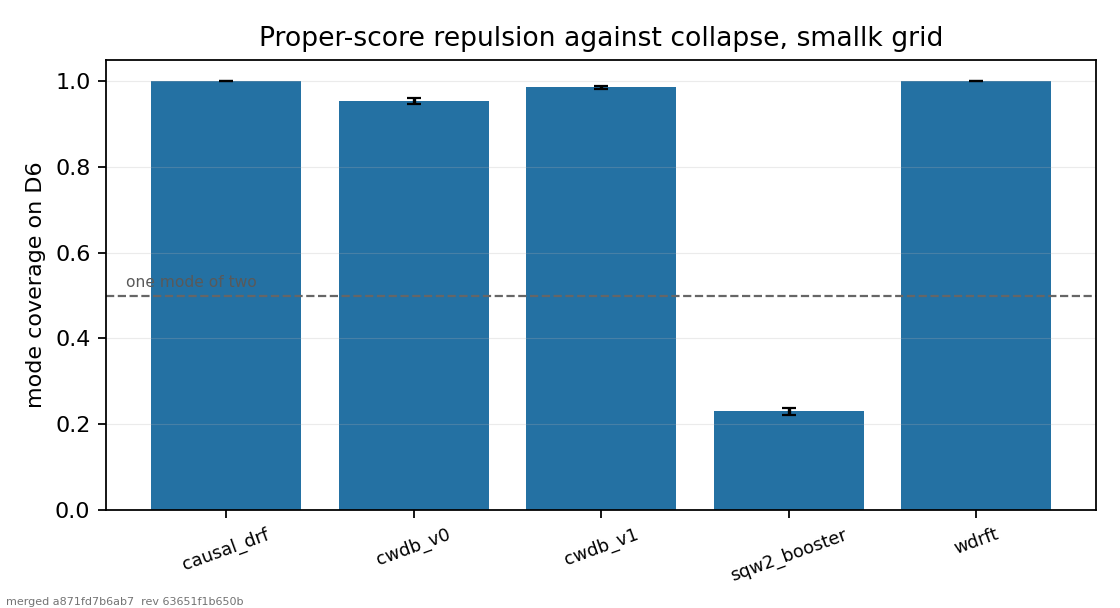
\includegraphics[width=0.86\textwidth]{../figures/simulation/mode_coverage_d6.png}
\caption{The repulsion ablation on D6. The squared-$W_2$ booster is the identical
tree machinery with the repulsion term of \eqref{eq:score} deleted; it collapses
below the level a single mode would give, while every law method that keeps the
term covers both modes.}
\label{fig:mode}
\end{figure}

\begin{figure}[htbp]
\centering
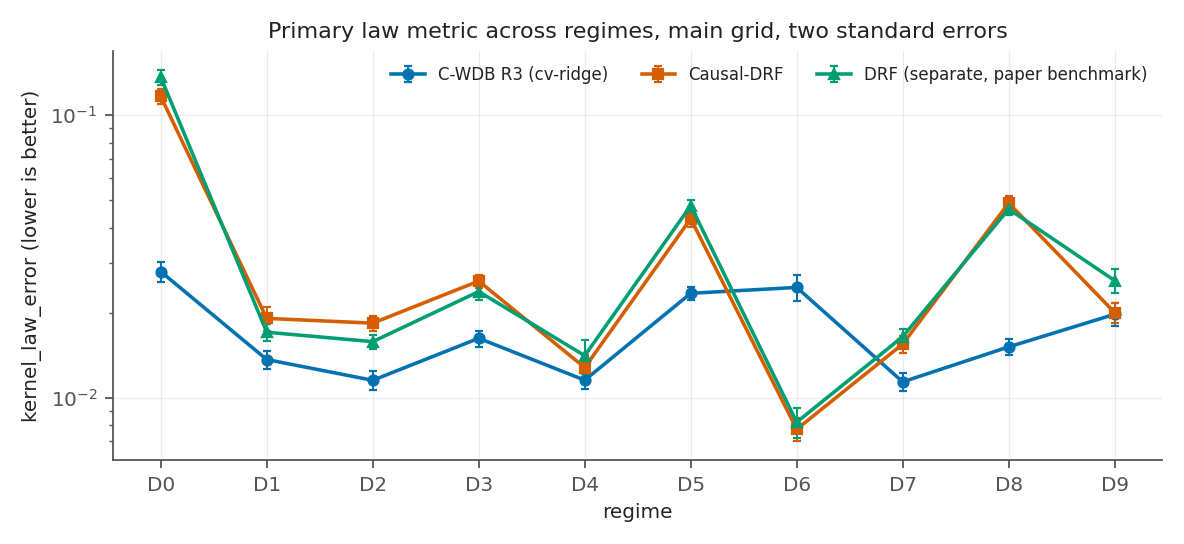
\includegraphics[width=0.94\textwidth]{figures_generated/kernel_all_regimes.png}
\caption{The declared primary law metric across all ten regimes on the main grid,
with two standard errors. Lower is better. The frozen claimant C-WDB-v1 and the
recommended repaired claimant C-WDB R3 are both shown, together with the two
forest baselines and the independent-arm ablation. Both C-WDB variants are at or
near the front almost everywhere; the exception is D6, discussed in the text.
Numbers behind this figure are in Table~\ref{tab:all-kernel}.}
\label{fig:crossover}
\end{figure}

\subsection{The adversarial reading}

The memo states the losses first, on the principle that averaging them into an
overall score would hide them. C-WDB-v1 is beaten by more than two paired
standard errors on twelve regime-target combinations, the most important of which
are collected in Table~\ref{tab:adverse}.

\begin{table}[htbp]
\centering
\caption{Selected cells where the claimant loses by more than two paired standard
errors. Positive differences favour the comparator.}
\label{tab:adverse}
\small
\begin{tabular}{@{}lllrrrr@{}}
\toprule
Regime & Target & Comparator & Claimant & Comparator & Difference & SE \\
\midrule
D6 & \texttt{kernel\_law\_error} & \texttt{causal\_drf} & 0.0191 & 0.00945 & $+0.00965$ & 0.00045 \\
D5 & \texttt{REF-ATE-K} & \texttt{causal\_drf} & 0.0937 & 0.0179 & $+0.0758$ & 0.0048 \\
D5 & \texttt{REF-TCATE-K} & \texttt{causal\_drf} & 0.0961 & 0.0230 & $+0.0730$ & 0.0046 \\
D6 & \texttt{REF-TCATE-K} & \texttt{causal\_drf} & 0.0746 & 0.0412 & $+0.0335$ & 0.0061 \\
D5 & \texttt{TCATE-K-grid\_sd} & \texttt{causal\_drf} & 0.0422 & 0.0275 & $+0.0146$ & 0.0024 \\
D7 & \texttt{TCATE-K-grid\_mean} & \texttt{pta\_s} & 0.0341 & 0.0223 & $+0.0118$ & 0.0041 \\
\bottomrule
\end{tabular}
\end{table}

Two of these matter for how the contribution is framed.

First, \CWDB{} loses the primary law metric on D6, the very regime built to
showcase its repulsion mechanism, while simultaneously dominating mode coverage
there. The two are consistent: the method places particles on both modes and so
wins any metric sensitive to missing a mode, but with only ten atoms it
represents the shape \emph{within} each mode more coarsely than a forest's
weighted empirical law over a thousand training points. This is a
representation-size effect, and the $M$-sensitivity evidence suggests raising $M$
narrows it slowly. Figure~\ref{fig:worst} shows D6 as the single red bar against
the incumbent.

Second, rule 4 passed on \textbf{zero accuracy wins and three capability wins}.
On every target where both methods produce an estimate, PTA-S is at least as
accurate. \CWDB{} passes only because on three targets PTA-S produces nothing at
all. That capability advantage is real and it is what a transfer test is for, but
the honest reading weakens it: PTA-S's remedy is to add the functional to its
manifest and fit one more scalar head, measured at 1.14 s. The capability gap is
a convenience advantage of seconds, not a barrier. Set against that, the
advantage over Causal-DRF, the published incumbent, \emph{is} an accuracy
advantage, on three of four eligible regimes for the primary law metric and on
five per-target functional comparisons. The incumbent comparison is the stronger
of the two, and the paper should be built on it.

\begin{figure}[htbp]
\centering
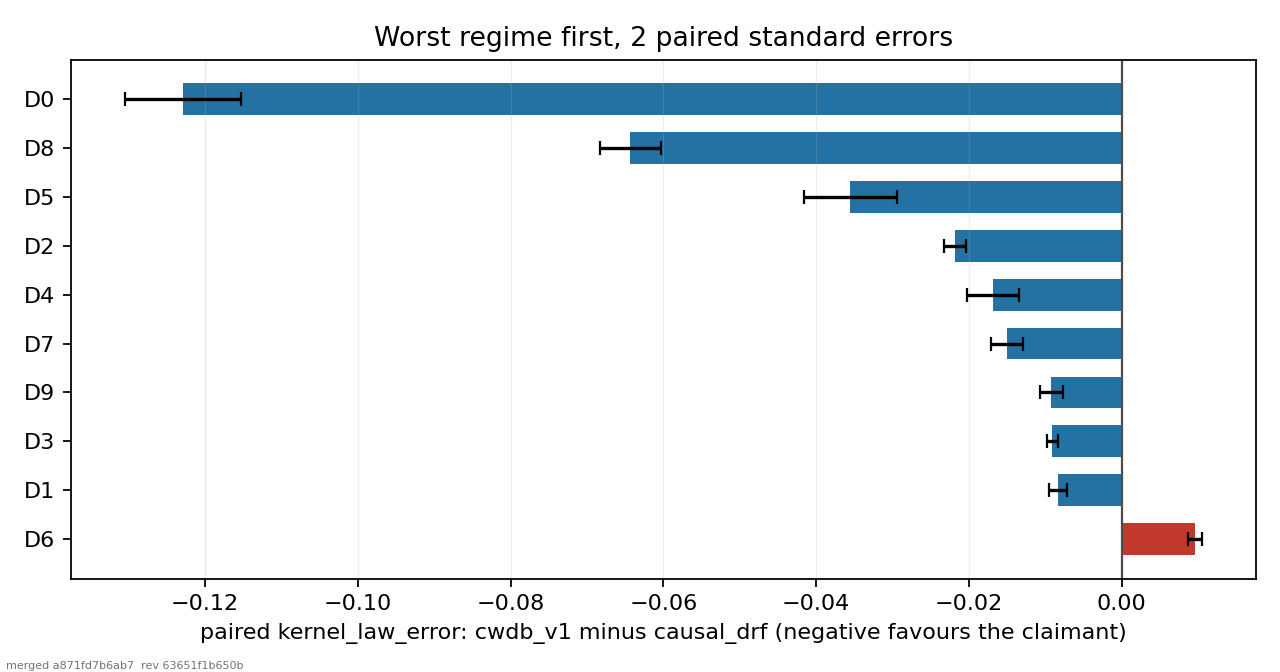
\includegraphics[width=0.9\textwidth]{../figures/simulation/worst_regime.png}
\caption{Paired primary-law-metric difference against the published incumbent,
worst regime first. Negative favours the claimant. Only D6 favours Causal-DRF.}
\label{fig:worst}
\end{figure}

\subsection{The recommended claimant placed in the same comparisons}
\label{sec:r3intournament}

Everything above is the frozen tournament, in which the only claimant was
C-WDB-v1. Because the repair track reuses the frozen coordinates and seeds
exactly (Section~\ref{sec:repair}), the recommended variant
\texttt{cwdb\_r3\_cvridge} can be dropped into precisely the same comparisons
without recomputing a single frozen number, and this subsection does that. The
complete metric-by-method tables are collected in Section~\ref{sec:complete};
what follows is the reading of them.

\begin{table}[htbp]
\centering
\caption{Where C-WDB R3 stands against the three comparators that matter, on the
frozen main grid. Read with Table~\ref{tab:paired-r3}, which gives every paired
difference and its standard error.}
\label{tab:r3-summary}
\small
\begin{tabular}{@{}lp{9.4cm}@{}}
\toprule
Comparator & Outcome for \texttt{cwdb\_r3\_cvridge} \\
\midrule
Causal-DRF (incumbent) & wins the primary law metric in nine of ten regimes,
losing only D6; wins the grid causal mean in six regimes, loses D1 and D5, ties
D4 and D9 \\
PTA-S (direct learner) & loses the grid causal mean in five regimes and wins two;
ties on most functionals both estimate; wins outright only on the two functionals
PTA-S cannot produce at all \\
C-WDB-v1 (frozen claimant) & improves six regimes on the grid causal mean, ties
two, regresses on D1 and D9, cuts the null-regime error by two thirds, and
\emph{loses the pure-shape transfer result} discussed below \\
\bottomrule
\end{tabular}
\end{table}

Four readings deserve stating in words rather than left in the tables, and the
fourth is the most important thing in this report that is not in either memo.

\emph{The incumbent comparison strengthens.} Figure~\ref{fig:pairedr3} is the
same construction as Figure~\ref{fig:worst} with the recommended variant in place
of the frozen one. The pattern is essentially unchanged: R3 wins nine of ten
regimes and D6 remains the only one the incumbent takes, with the margins within
a hair of the frozen claimant's (larger for R3 in four regimes, smaller in five,
and the D6 loss itself smaller at $+0.0131$ against $+0.0163$). The law-level
advantage is therefore preserved rather than improved, which is the point: the
contrast rule was not supposed to move the pooled fit and the numbers say it did
not. On the grid causal mean, where the contrast \emph{is} the estimand, the D8
advantage is now dramatic, $0.0735$ against Causal-DRF's $0.3769$.

\emph{The null regime is no longer a liability.} On D2 the grid causal mean falls
from v1's $0.1466$ to $0.0506$, which is \emph{below} the best baseline's
$0.0545$ rather than $2.69$ times it. Figure~\ref{fig:contrastrules} shows what
each contrast rule pays for that: the cross-fitted rule is the only one that
clears the cap on D2 while leaving D0 and D3 essentially where the frozen
claimant left them.

\emph{The direct target learner is still the one to beat on the common target.}
On the grid causal mean, PTA-S beats R3 in five regimes (D0, D1, D4, D5, D9) and
loses in two (D3, D8). Nothing in the repair changes the parent memo's judgement
that this comparison is the weak part of the case.

\emph{The repair damages the pure-shape transfer result, and this is not
reported anywhere else in the project's artefacts.} The clearest single result of
the frozen tournament was D7's \texttt{TCATE-K-grid\_skewness}, where C-WDB-v1
scored $0.0152$ against Causal-DRF's $0.0840$, a factor of five and a half on the
functional carrying that regime's entire treatment effect. Every contrast rule
degrades it, in proportion to how hard it shrinks:

\begin{table}[htbp]
\centering
\caption{D7 \texttt{TCATE-K-grid\_skewness}, the functional that carries the whole
D7 treatment effect and appears in no training manifest. The middle column is the
paired difference against the frozen claimant, the right column against the
published incumbent. Positive is worse.}
\label{tab:d7skew}
\small
\begin{tabular}{@{}lrrr@{}}
\toprule
Method & Error & vs C-WDB-v1 & vs Causal-DRF \\
\midrule
\texttt{cwdb\_v1} & 0.0152 & --- & $-0.0688$ (0.0028) \\
\texttt{cwdb\_v1\_pooledinit} & 0.0253 & $+0.0101$ (0.0015) & $-0.0587$ (0.0030) \\
\texttt{cwdb\_r1\_ridge} & 0.0645 & $+0.0493$ (0.0027) & $-0.0195$ (0.0029) \\
\texttt{cwdb\_r3\_cvridge} & 0.0904 & $+0.0752$ (0.0069) & $+0.0064$ (0.0074) \\
\texttt{cwdb\_r2\_threshold3} & 0.1986 & $+0.1834$ (0.0052) & $+0.1146$ (0.0046) \\
\midrule
\texttt{causal\_drf} & 0.0840 & & \\
\texttt{wdrft} & 0.0464 & & \\
\texttt{pta\_s} & \emph{n/a} & & \\
\bottomrule
\end{tabular}
\end{table}

The mechanism is not mysterious and it follows directly from
Section~\ref{sec:armtree}. D7 places the entire effect in the arm contrast of the
inner shape, and a contrast regulariser shrinks exactly that. Cross-fitting
selects a median strength of 50 on D7, so it shrinks a contrast that is real. The
result is that R3 ties the incumbent on this functional instead of beating it by
a factor of five, and \texttt{cwdb\_r2\_threshold3} loses to the incumbent
outright. The effect is not an artefact of one grid or one estimand: it
reproduces at $K = 5$ ($0.0629$ for R3 against $0.0095$ for v1) and on the
marginal \texttt{TATE-K-grid\_skewness} ($0.0746$ against $0.0070$), where R3 is
also worse than both forest baselines.

Two things keep this from being fatal, and both belong in the same breath as the
finding. First, the transfer claim does not rest on skewness alone: on D7's
\texttt{TCATE-K-grid\_upper\_tail\_mean}, the other functional excluded from
every training manifest, R3 still beats Causal-DRF ($0.0314$ against $0.0821$)
and PTA-S still cannot produce it. Second, the gate rules were satisfied on their
own terms, because rules 3 and 4 are evaluated over the declared target set and
not over skewness specifically. But a paper whose headline example is the
skewness result cannot be written around \texttt{cwdb\_r3\_cvridge} as if the
repair were free, and an applied study that targets a pure shape contrast should
expect the regularised claimant to be conservative about exactly that contrast.

Figure~\ref{fig:functionals} shows all four functionals across the three eligible
regimes and makes the trade visible in one picture.

\begin{figure}[htbp]
\centering
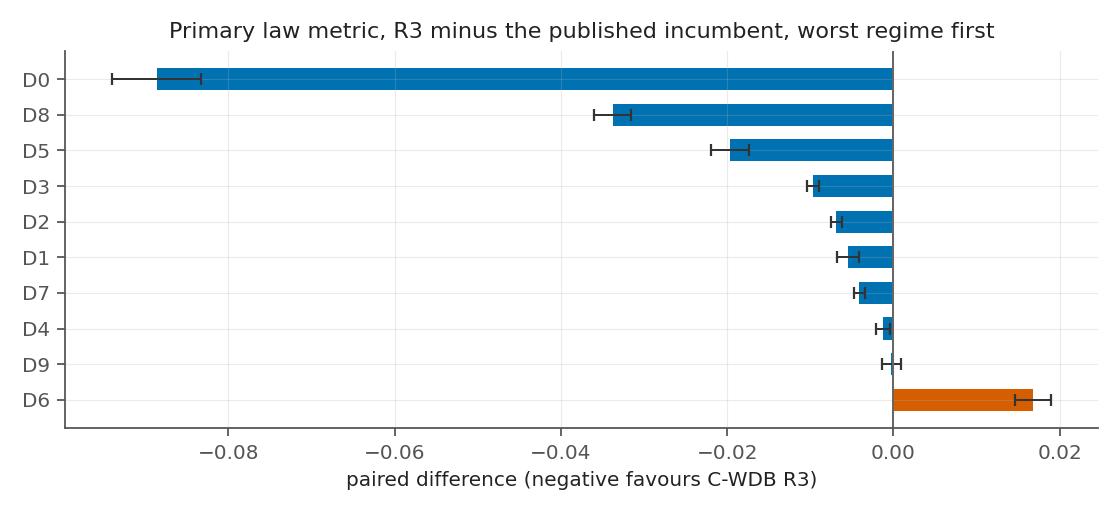
\includegraphics[width=0.9\textwidth]{figures_generated/paired_r3_vs_drf.png}
\caption{Paired primary-law-metric difference of the recommended claimant against
the published incumbent, worst regime first, two paired standard errors. Negative
favours C-WDB R3. Compare Figure~\ref{fig:worst}, which is the same construction
for the frozen claimant.}
\label{fig:pairedr3}
\end{figure}

\begin{figure}[htbp]
\centering
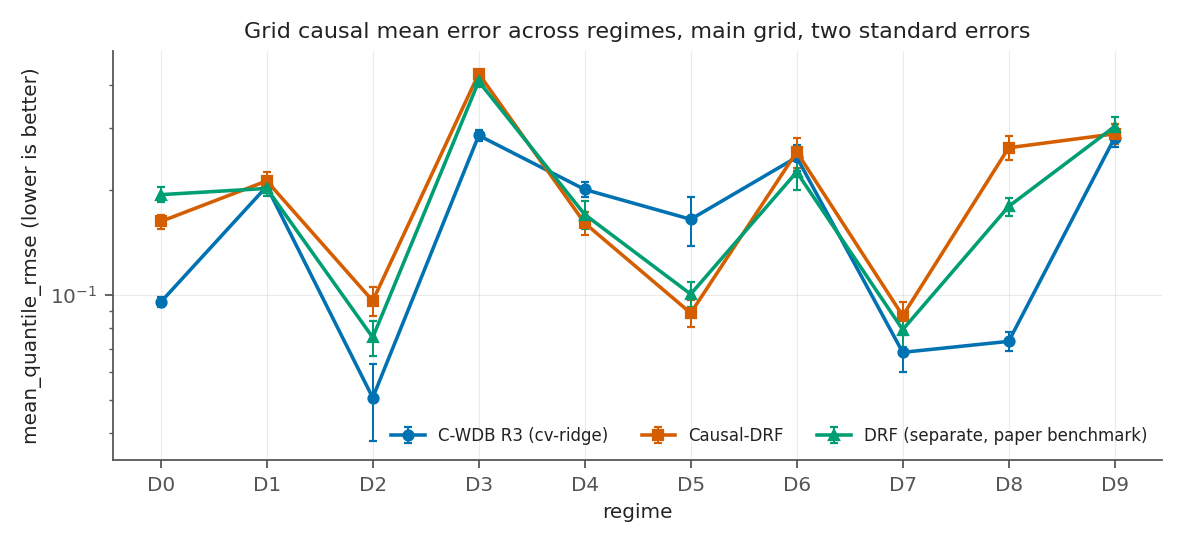
\includegraphics[width=0.94\textwidth]{figures_generated/meanq_all_regimes.png}
\caption{Grid causal mean error, the mandatory common target every method can
produce, across all ten regimes. The D2 gap between the two C-WDB curves is the
repair. PTA-S is the strongest comparator on this metric and remains so in six
regimes, which is the honest statement of where a direct target learner is hard
to beat. Numbers in Table~\ref{tab:all-meanq}.}
\label{fig:meanq}
\end{figure}

\begin{figure}[htbp]
\centering
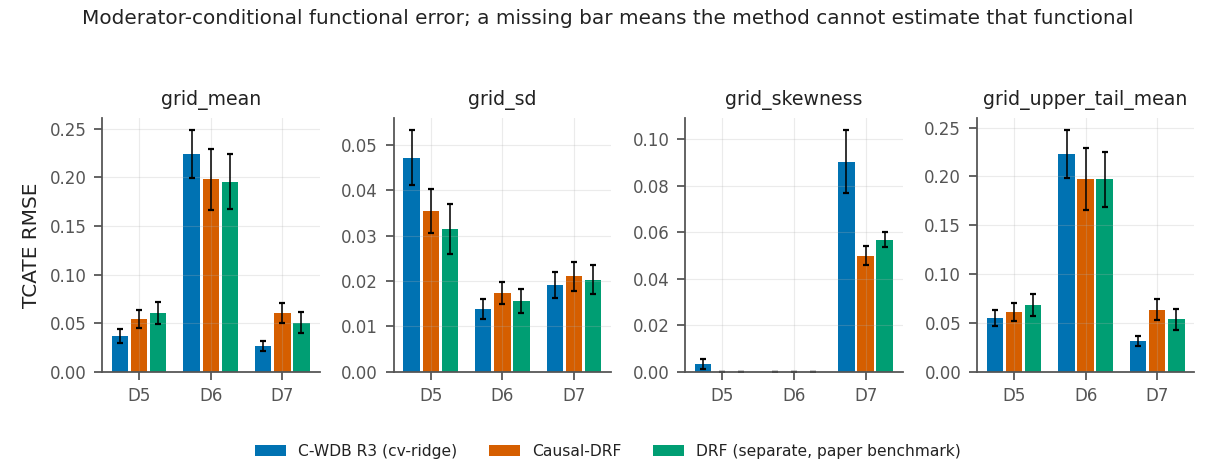
\includegraphics[width=0.98\textwidth]{figures_generated/functional_targets.png}
\caption{Moderator-conditional functional error on the three regimes eligible for
the transfer rules. \texttt{grid\_skewness} and \texttt{grid\_upper\_tail\_mean}
are excluded from every training manifest, so PTA-S is marked \emph{n/a} there:
that is the transfer test, not a missing measurement. On D6 the true skewness
effect is numerically zero, which is why that panel's bars vanish for every
method. Numbers in Table~\ref{tab:all-tcate}.}
\label{fig:functionals}
\end{figure}

\begin{figure}[htbp]
\centering
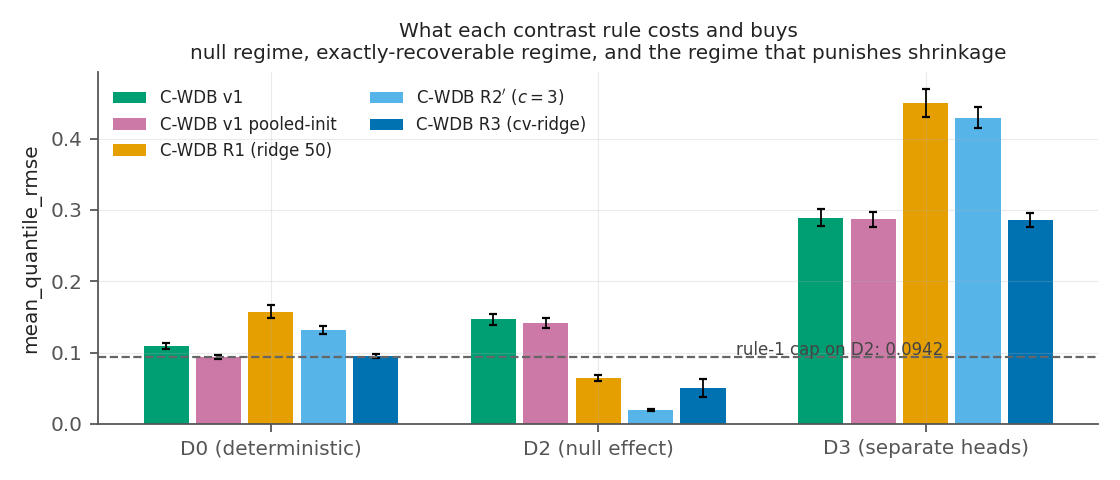
\includegraphics[width=0.9\textwidth]{figures_generated/contrast_rules_d0_d2_d3.png}
\caption{What each contrast rule costs and buys, on the grid causal mean. D2 is
the null regime the gate failed on and the dashed line is its preregistered cap.
D0 is exactly recoverable, so a rule that cannot switch itself off is penalised
there, which is what happens to the hand-tuned fixed ridge. D3 is built to favour
separate heads, so a rule that shrinks every contrast is penalised there, which
is what happens to both fixed rules. Only the cross-fitted rule is acceptable in
all three.}
\label{fig:contrastrules}
\end{figure}

\subsection{Finite-particle approximation}
\label{sec:particles}

\begin{table}[htbp]
\centering
\caption{Excess energy risk over the true law as a function of the particle
count, 20 replications each.}
\label{tab:particles}
\small
\begin{tabular}{@{}lrrrr@{}}
\toprule
Regime & $M=2$ & $M=5$ & $M=10$ & $M=25$ \\
\midrule
D1 & 0.0897 & 0.0584 & 0.0508 & 0.0468 \\
D6 & 0.1063 & 0.0851 & 0.0696 & 0.0651 \\
\bottomrule
\end{tabular}
\end{table}

Excess risk falls monotonically in $M$ and is nearly flat past $M=10$
(Figure~\ref{fig:particles}). Ten particles buy most of what twenty-five buy,
which is what keeps the method at 11.3 times the incumbent's runtime rather than
far more. This is the empirical counterpart to the fixed-$M$ contract of
Section~\ref{sec:finiteM}: the approximation is real, it is measured, and it is
small at the operating point.

\begin{figure}[htbp]
\centering
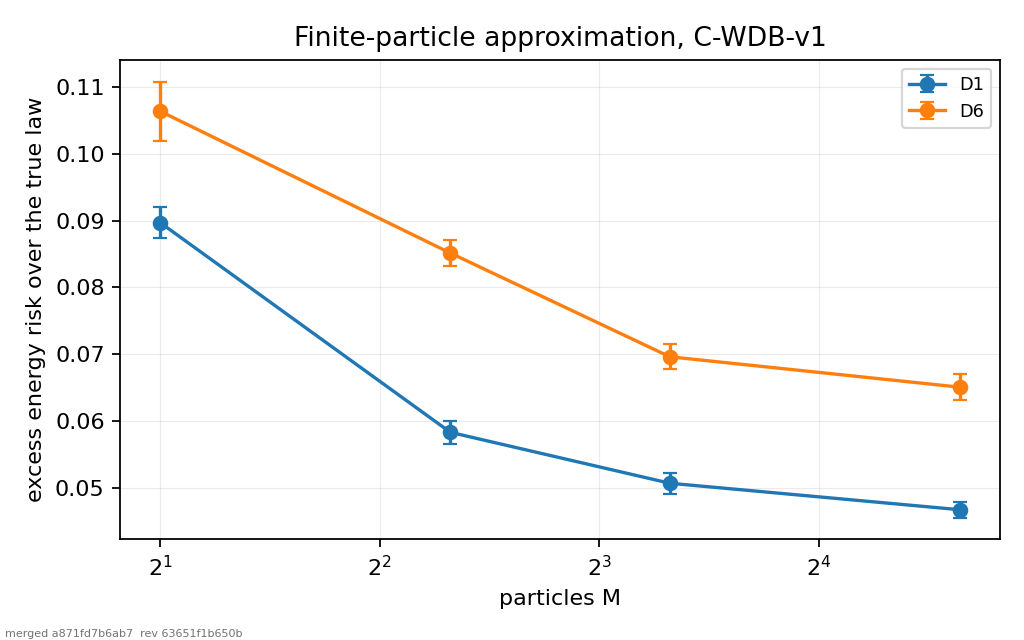
\includegraphics[width=0.66\textwidth]{../figures/simulation/particle_sensitivity.png}
\caption{Finite-particle approximation error. The vertical axis is excess energy
risk over the true conditional law, so zero is attainable only by the truth.}
\label{fig:particles}
\end{figure}

\subsection{Cost}

\begin{table}[htbp]
\centering
\caption{Runtime and memory across the whole tournament.}
\label{tab:cost}
\small
\begin{tabular}{@{}lrrr@{}}
\toprule
Method & Median runtime (s) & Max runtime (s) & Median peak RSS (MB) \\
\midrule
\texttt{causal\_drf} & 1.17 & 35.4 & 75.2 \\
\texttt{sqw2\_booster} & 1.00 & 2.3 & 0 \\
\texttt{wdrft} & 1.33 & 36.2 & 214 \\
\texttt{cwdb\_v0} & 8.93 & 42.2 & 0 \\
\texttt{cwdb\_v1} & 13.3 & 149 & 0 \\
\texttt{pta\_s} & 28.1 & 77.4 & 0 \\
\texttt{pta\_f} & 96.1 & 113 & 0 \\
\bottomrule
\end{tabular}
\end{table}

\section{Diagnosis of the rule-1 failure}
\label{sec:diagnosis}

Two distinct mechanisms produced the false effect on D2, and separating them
before writing any fix changed which repair was worth building. Both diagnostics
ran on pilot seeds outside the manifest.

\subsection{Defect one: confounded initialization}

\texttt{compute\_init\_base} was applied per arm, so each arm started from the
empirical law of its own treated or control sample. That is a \emph{marginal}
quantity. Under a covariate-dependent propensity the two marginals differ even
when the two conditional laws are identical, so the estimated contrast is nonzero
before a single tree is fitted, and the booster then spends its budget removing an
offset the initialization created. Measured over 20 samples at $n = 1000$, the
initial arm gap has root mean square $0.215$ on D2, where the truth is exactly
zero, and $0.824$ on D8.

\subsection{Defect two: contrast accumulation}

Replaying the fitted path on a held-out design, D2's contrast error reaches a
minimum near iteration 20 and then rises \emph{monotonically} to the frozen
budget of 100: $0.077, 0.093, 0.104, 0.114, 0.122$ at iterations
$20, 40, 60, 80, 100$. Repeating the sweep at \texttt{arm\_shrinkage} of $0$,
$50$, and $500$ gives final errors of $0.161$, $0.076$, and $0.045$, which
locates the defect precisely. As Section~\ref{sec:armtree} shows, the frozen rule
leaves a contrast of $n_a/(n_a+\lambda) \approx 0.86$ of the raw gap at a typical
leaf. The contrast was barely regularized at all, and one hundred boosting steps
compounded what survived.

\subsection{Attribution}

The initialization ablation settles which defect is the repair.
\texttt{cwdb\_v1\_pooledinit} is frozen v1 in every respect except that both arms
start from one pooled base law. It improves D2 from $0.1466$ to $0.1419$, a
false-effect ratio of $2.60$ against $2.69$, and \textbf{still fails rule 1}. The
initialization was a genuine defect and fixing it was free, but it is not the
repair. The second mechanism is.

\section{The repair track}
\label{sec:repair}

\subsection{Design}

The repair preregistration amends nothing in the parent document: every
threshold, metric, eligible regime, decision multiple, and comparator stays as
frozen. It adds methods and cells only. The 97{,}650 frozen rows were \emph{not}
recomputed, so a repair variant is compared against the numbers already
published rather than a fresh draw of them, and repair cells reuse the frozen
coordinates and seeds so every comparison is paired seed by seed.

The run was staged deliberately. Stage 1 is D2 alone, because rule 1 is the only
rule the repair exists to fix and a variant that fails to fix it should cost
nothing further; stage 2 runs every regime and the two ablation grids, and only
for variants that cleared stage 1. Execution: 2600 repair cells, 68{,}240 rows,
zero failures, merge audit \texttt{PASS}, independent recomputation agreeing with
zero disagreements, and the frozen gate flags byte-identical to the published
payload.

\subsection{Rule 1 across the roster}

\begin{table}[htbp]
\centering
\caption{Rule 1 for every variant. The D2 reference is the best of the frozen
roster, 0.0545, which a repair variant cannot move by entering the pool. The D0
cap is 0.15 and the D2 ratio cap is 1.25.}
\label{tab:rule1}
\small
\begin{tabular}{@{}lrrrl@{}}
\toprule
Method & D2 \texttt{mean\_quantile\_rmse} & Ratio & D0 & Rule 1 \\
\midrule
\texttt{cwdb\_v1} (frozen claimant) & 0.1466 & 2.69 & 0.1091 & \textbf{FAIL} \\
\texttt{cwdb\_v1\_pooledinit} (ablation) & 0.1419 & 2.60 & 0.0939 & \textbf{FAIL} \\
\texttt{cwdb\_r1\_ridge} ($\lambda_\tau = 50$) & 0.0642 & 1.18 & 0.1574 & \textbf{FAIL} \\
\texttt{cwdb\_r2\_threshold} ($c=1$) & 0.0790 & 1.45 & not run & \textbf{FAIL} \\
\texttt{cwdb\_r2\_threshold3} ($c=3$) & 0.0194 & 0.36 & 0.1322 & PASS \\
\texttt{cwdb\_r3\_cvridge} & 0.0506 & 0.93 & 0.0952 & PASS \\
\bottomrule
\end{tabular}
\end{table}

Two entries need stating in words. The hand-tuned fixed ridge R1 clears the D2
ratio at $1.18$ and then fails rule 1 anyway, \emph{on D0}, at $0.1574$ against a
cap of $0.15$. D0 has deterministic conditional distributions, so its conditional
mean is exactly recoverable, and a fixed contrast shrinkage that cannot switch
itself off biases the recoverable answer. R1 is the one variant that was tuned,
it was tuned on D2, and it broke the regime it was not tuned on. That is the
argument against a frozen strength, made by the frozen strength itself.

R2 at the principled null-calibrated $c = 1$ missed the cap at $1.45$ and stopped
after D2 under the preregistered screen. Its rows remain in the merged table and
in the memo. The calibration that is principled is not the one that passed; the
one that passed, $c = 3$, is a declared conservative sensitivity, and that
ordering is reported rather than smoothed over.

\subsection{All six rules}

\begin{table}[htbp]
\centering
\caption{Gate outcome for every repair variant.}
\label{tab:gate2}
\small
\begin{tabular}{@{}lcccccccl@{}}
\toprule
Method & 1 & 2 & 3 & 4 & 5 & 6 & & Verdict \\
\midrule
\texttt{cwdb\_v1} & fail & PASS & PASS & PASS & PASS & PASS & & \texttt{NOT-GO} \\
\texttt{cwdb\_v1\_pooledinit} & fail & PASS & PASS & PASS & PASS & PASS & & \texttt{NOT-GO} \\
\texttt{cwdb\_r1\_ridge} & fail & PASS & PASS & PASS & PASS & PASS & & \texttt{NOT-GO} \\
\texttt{cwdb\_r2\_threshold3} & PASS & PASS & PASS & PASS & PASS & PASS & & \textbf{\texttt{GO}} \\
\texttt{cwdb\_r3\_cvridge} & PASS & PASS & PASS & PASS & PASS & PASS & & \textbf{\texttt{GO}} \\
\bottomrule
\end{tabular}
\end{table}

Rule 2 holds for both passing variants with three wins against Causal-DRF on the
primary law metric, in D1, D5, and D7, the same three regimes the frozen claimant
won. Rule 5 holds for both, with D6 mode coverage $0.9921$ and $0.9931$ against
the frozen claimant's $0.9897$ and participation at $10.00$ of $M = 10$ in every
case. The repulsion mechanism is untouched, which is the point of the
reparameterization \eqref{eq:reparam}: the contrast rules move only the arm gap
and provably cannot move the pooled component.

Rule 6, against the original-code Causal-DRF median of $8.77$ s and a ceiling of
60, gives R3 a median of $55.35$ s and a ratio of $6.3$.
The repair preregistration recorded, before the run, that R3 was projected near
64 and might fail; it landed at 55.35 because the projection applied the factor
measured on the expensive $K=25$ cells to every cell, whereas the cheap $K=5$
cells carry a smaller multiplier and the median sits among them. The projection
was pessimistic; the budget was not revised after the fact.

\subsection{What separates the two passing variants}

Both pass. They are not equally good, and the mechanism ablations say why.

\begin{table}[htbp]
\centering
\caption{Mechanism ablations, paired differences with standard errors in
parentheses. Negative favours the claimant. Bold marks the ablation that is lost.}
\label{tab:ablations}
\footnotesize
\setlength{\tabcolsep}{4pt}
\begin{tabular}{@{}llrrr@{}}
\toprule
Ablation & Comparator & \texttt{cwdb\_v1} & \texttt{cwdb\_r2\_threshold3} & \texttt{cwdb\_r3\_cvridge} \\
\midrule
Repulsion, D6 mode coverage & \texttt{sqw2\_booster} & $-0.7550$ (0.0050) & $-0.7581$ (0.0064) & $-0.7584$ (0.0061) \\
Repulsion, D6 law metric & \texttt{sqw2\_booster} & $-0.1602$ (0.0012) & $-0.1646$ (0.0010) & $-0.1646$ (0.0012) \\
Sharing, D3 mean-quantile & \texttt{cwdb\_v0} & $-0.0320$ (0.0036) & $\mathbf{+0.0944}$ (0.0042) & $-0.0306$ (0.0030) \\
Sharing, D3 law metric & \texttt{cwdb\_v0} & $-0.0001$ (0.0003) & $\mathbf{+0.0055}$ (0.0004) & $-0.0001$ (0.0003) \\
Sharing, D4 mean-quantile & \texttt{cwdb\_v0} & $-0.1012$ (0.0032) & $-0.0805$ (0.0062) & $-0.1003$ (0.0039) \\
Shrinkage, D2 mean-quantile & \texttt{cwdb\_v1\_noshrink} & $-0.0338$ (0.0015) & $-0.1431$ (0.0018) & $-0.1188$ (0.0037) \\
Shrinkage, D8 mean-quantile & \texttt{cwdb\_v1\_noshrink} & $-0.0320$ (0.0027) & $-0.1336$ (0.0051) & $-0.1420$ (0.0042) \\
\bottomrule
\end{tabular}
\end{table}

\texttt{cwdb\_r2\_threshold3} \textbf{loses the sharing ablation on D3}, reaching
$0.3854$ against C-WDB-v0's $0.2910$, and loses the law metric there too. D3 is
the regime built to favour separate heads, and a rule that shrinks every arm gap
toward the pooled leaf is punished by exactly the structure D3 contains. The
shared-partition mechanism is one of the project's own claims and the parent memo
supports it with this ablation, so a repair that passes the gate and takes that
claim with it has traded one asset for another. R1 loses the same ablation for
the same reason.

\texttt{cwdb\_r3\_cvridge} keeps it, at $-0.0306$ (SE 0.0030), matching the
frozen claimant's $-0.0320$ (SE 0.0036) to within a standard error. It loses
exactly one ablation, D1 kernel law error against the squared-$W_2$ booster,
which is the same one the frozen claimant already lost and is therefore not
damage the repair caused.

The reason is visible in what cross-fitting selects (Table~\ref{tab:selected}).
On D3 it selects zero strength on every seed, so the shared-partition mechanism
runs unregularized where the data say a real contrast exists; on D2 and D8 it
selects hard. That is the adaptivity a fixed rule cannot have, and it is what
lets one variant repair rule 1 without paying for it anywhere else.

\begin{table}[htbp]
\centering
\caption{Median contrast strength selected on held-out energy risk by
\texttt{cwdb\_r3\_cvridge}.}
\label{tab:selected}
\small
\begin{tabular}{@{}llp{7.2cm}@{}}
\toprule
Regimes & Median strength & What the regime contains \\
\midrule
D0, D3 & 0 & deterministic laws; strong separate-head effect \\
D1, D4, D5 & 0 & moderate real effects \\
D2 & 50 (mean 265) & exactly null effect \\
D6, D7, D9 & 50 & multimodal; unseen-functional effect; poor overlap \\
D8 & 500 & strong confounding, weak effect \\
\bottomrule
\end{tabular}
\end{table}

\subsection{Improvement beyond the rule that failed}

\begin{table}[htbp]
\centering
\caption{\texttt{cwdb\_r3\_cvridge} against \texttt{cwdb\_v1} on
\texttt{mean\_quantile\_rmse}, main grid, paired by seed.}
\label{tab:r3vs}
\small
\begin{tabular}{@{}lrrrrl@{}}
\toprule
Regime & R3 & v1 & Difference & SE & Favours \\
\midrule
D0 & 0.0872 & 0.1013 & $-0.0141$ & 0.0025 & repair \\
D1 & 0.1809 & 0.1691 & $+0.0118$ & 0.0027 & v1 \\
D2 & 0.0417 & 0.1266 & $-0.0850$ & 0.0037 & repair \\
D3 & 0.2603 & 0.2590 & $+0.0014$ & 0.0022 & tie \\
D4 & 0.1774 & 0.1765 & $+0.0009$ & 0.0032 & tie \\
D5 & 0.0910 & 0.1559 & $-0.0649$ & 0.0099 & repair \\
D6 & 0.2130 & 0.2490 & $-0.0360$ & 0.0094 & repair \\
D7 & 0.0572 & 0.1264 & $-0.0692$ & 0.0020 & repair \\
D8 & 0.0641 & 0.1741 & $-0.1100$ & 0.0062 & repair \\
D9 & 0.2442 & 0.2211 & $+0.0231$ & 0.0095 & v1 \\
\bottomrule
\end{tabular}
\end{table}

Six regimes improve, two tie, and two regress. The regressions are D1, a smooth
location-scale law with a real effect, and D9, where overlap deteriorates to the
clipping bounds. Both are small in absolute terms and both are cases where
regularizing a real contrast costs something; neither is a gate rule and neither
should be described as free. The largest single improvement is D8, from $0.1741$
to $0.0641$, which is exactly the regime combining both diagnosed defects: its
initialization gap was $0.824$ and its effect is weak enough that accumulated
contrast noise dominates it.

\subsection{Recommendation}

Adopt \texttt{cwdb\_r3\_cvridge} as the claimant. It is the only variant that
repairs rule 1 while leaving every mechanism the project claims as its own
intact, and the mechanism that makes that possible, choosing the regularization
strength on held-out energy risk rather than freezing it, is the one the parent
memo asked for by name.

Report \texttt{cwdb\_r2\_threshold3} alongside it, not as a rejected alternative
but as the variant that buys three \emph{accuracy} wins over PTA-S (at D6
\texttt{TCATE-K-grid\_sd}, D7 \texttt{TCATE-K-grid\_mean}, D7
\texttt{TCATE-K-grid\_sd}) at the price of the shared-partition ablation. A
reader who cares more about the direct-learner comparison than about the sharing
claim would prefer it, and the results say so. Neither variant dominates.


\clearpage
\section{Complete results: every metric for the proposed model and comparators}
\label{sec:complete}

The sections above argue from selected comparisons. This section reports the
whole measurement surface so that a reader can check any claim in the report, or
find one it did not make. The tables intentionally retain only
\texttt{cwdb\_r3\_cvridge} as the proposed C-WDB model, together with the
original-code Causal-DRF incumbent and the original-code separate-DRF benchmark.
PTA-S, PTA-F, and the earlier W-DRF-T adapter are not part of this core
comparison. Nothing here is recomputed: the tables are generated
directly from the audited result files by
\texttt{report/build\_report\_assets.py}, which reads and aggregates but never
fits a model. The Causal-DRF columns use the original-code rerun recorded in
\texttt{results/merged\_original\_causal\_drf}, not the earlier local driver.
The DRF columns use the separate half-sample implementation in
\texttt{code/drfinference-main}, with 2500 total trees and 50 trees per group.
The selected historical discussion above preserves the original tournament
record; the tables and figures in this section are the corrected comparator
record.

\paragraph{Conventions.} Every entry is a mean over cells with the standard error
in parentheses. A cell is one (grid, regime, $n$, $K$, $M$, method, seed)
combination, and arm-specific rows are averaged inside a cell first, matching the
convention of the independent gate-flag recomputation. On the \texttt{main} grid
that is 40 cells per entry, $n \in \{500, 1000\}$ crossed with 20 seeds; on
\texttt{smallk} it is 20 cells at $n = 500$, $K = 5$. Bold marks the best method
in a regime. \emph{n/a} means the method does not produce that quantity at all,
which for the two PTA endpoints is a contract restriction rather than a
measurement gap, and for \texttt{cwdb\_r2\_threshold} at $c = 1$ is the
preregistered stage-1 screen that stopped it after D2.

\paragraph{Reading the comparator.} The squared-$W_2$ booster appears only on
the small-$K$ mechanism tables as a comparator for the repulsion term. It is not
a proposed model. The DRF column is the faithful separate-forest benchmark from
the Causal-DRF paper, whereas W-DRF-T is deliberately excluded from this core
comparison because it is a different, cheaper adapter.

\paragraph{Treatment-effect reading.} This focused comparison is more relevant
to the contribution than a leaderboard containing fixed-target mean learners.
On the main grid, R3 is the lowest-error method in six of ten regimes for
\texttt{mean\_quantile\_rmse}, seven of ten for \texttt{REF-TCATE-K}, and five
of ten for \texttt{REF-ATE-K}. Across the forty conditional functional cells,
R3 is best in twenty-four, compared with eleven for DRF and five for
Causal-DRF. Across the forty marginal functional cells, R3 is best in
twenty-eight, compared with eight for DRF and four for Causal-DRF. These are
cell-average rankings, not a claim of uniform dominance or a replacement for
the paired standard errors in Table~\ref{tab:paired-r3}.

The most relevant transfer regime is D7. R3 is best for the conditional mean,
standard deviation, and upper-tail effect, and for all three corresponding
marginal effects. It loses the D7 skewness effect to both forest comparators:
the conditional errors are $0.0904$ for R3, $0.0500$ for Causal-DRF, and
$0.0567$ for DRF. The result supports a narrower and stronger claim: R3 is
especially effective for marginal and tail treatment-effect functionals, while
pure skewness contrasts remain a documented failure region.

\paragraph{One caution about pooled means.} A regime mean pools $n = 500$ and
$n = 1000$, so it is not identical to the per-$n$ numbers quoted in the repair
memo's Section 6, which are $n = 1000$. Both conventions appear in the project;
this report uses the pooled one everywhere except where it says otherwise, which
is the same convention rule 1 is evaluated under.

\begin{landscape}
\paragraph{Column abbreviations.} The wide tables use short method names:
R3 is \texttt{cwdb\_r3\_cvridge}, C-DRF is Causal-DRF, DRF is the separate
half-sample forest benchmark from the original Causal-DRF code, and sq-$W_2$ is
the repulsion ablation.

\begin{table}[htbp]
\centering
\caption{Grid causal mean error \texttt{mean\_quantile\_rmse} against \texttt{MEANQ-A-K}, main grid, mean over 40 cells ($n\in\{500,1000\}$, 20 seeds) with the standard error in parentheses. Best in each regime is bold.}
\label{tab:all-meanq}
\scriptsize
\setlength{\tabcolsep}{3.2pt}
\begin{tabular}{@{}lrrr@{}}
\toprule
Regime & R3 & C-DRF & DRF \\
\midrule
D0 & \textbf{0.0952\,(0.0016)} & 0.1621\,(0.0038) & 0.1935\,(0.0048) \\
D1 & 0.2043\,(0.0042) & 0.2119\,(0.0062) & \textbf{0.2017\,(0.0049)} \\
D2 & \textbf{0.0506\,(0.0063)} & 0.0960\,(0.0046) & 0.0754\,(0.0042) \\
D3 & \textbf{0.2861\,(0.0049)} & 0.4301\,(0.0060) & 0.4088\,(0.0072) \\
D4 & 0.2002\,(0.0048) & \textbf{0.1603\,(0.0062)} & 0.1697\,(0.0078) \\
D5 & 0.1644\,(0.0133) & \textbf{0.0885\,(0.0038)} & 0.1004\,(0.0041) \\
D6 & 0.2477\,(0.0108) & 0.2567\,(0.0128) & \textbf{0.2247\,(0.0129)} \\
D7 & \textbf{0.0683\,(0.0042)} & 0.0870\,(0.0042) & 0.0794\,(0.0043) \\
D8 & \textbf{0.0735\,(0.0022)} & 0.2638\,(0.0104) & 0.1790\,(0.0053) \\
D9 & \textbf{0.2819\,(0.0087)} & 0.2891\,(0.0095) & 0.3034\,(0.0101) \\
\bottomrule
\end{tabular}
\par\vspace{2pt}\parbox{\textwidth}{\scriptsize \texttt{cwdb\_r2\_threshold} at $c=1$ is omitted: the preregistered stage-1 screen stopped it after D2, where it scored 0.0790.}
\end{table}

\begin{table}[htbp]
\centering
\caption{Declared primary law metric \texttt{kernel\_law\_error} (squared MMD to the true conditional law, Gaussian kernel on the rescaled coordinates, median bandwidth), main grid, for the two forest comparators and the proposed law estimator.}
\label{tab:all-kernel}
\scriptsize
\setlength{\tabcolsep}{3.2pt}
\begin{tabular}{@{}lrrr@{}}
\toprule
Regime & R3 & C-DRF & DRF \\
\midrule
D0 & \textbf{0.0280\,(0.0012)} & 0.1166\,(0.0035) & 0.1365\,(0.0044) \\
D1 & \textbf{0.0137\,(0.0005)} & 0.0191\,(0.0009) & 0.0171\,(0.0006) \\
D2 & \textbf{0.0115\,(0.0004)} & 0.0184\,(0.0006) & 0.0158\,(0.0005) \\
D3 & \textbf{0.0162\,(0.0005)} & 0.0259\,(0.0007) & 0.0238\,(0.0008) \\
D4 & \textbf{0.0115\,(0.0004)} & 0.0128\,(0.0007) & 0.0141\,(0.0010) \\
D5 & \textbf{0.0234\,(0.0006)} & 0.0431\,(0.0013) & 0.0478\,(0.0012) \\
D6 & 0.0246\,(0.0013) & \textbf{0.0077\,(0.0004)} & 0.0082\,(0.0005) \\
D7 & \textbf{0.0114\,(0.0004)} & 0.0155\,(0.0005) & 0.0165\,(0.0005) \\
D8 & \textbf{0.0151\,(0.0005)} & 0.0489\,(0.0014) & 0.0466\,(0.0011) \\
D9 & \textbf{0.0197\,(0.0009)} & 0.0200\,(0.0008) & 0.0260\,(0.0013) \\
\bottomrule
\end{tabular}
\end{table}

\begin{table}[htbp]
\centering
\caption{Excess energy risk over the true conditional law \texttt{arm\_energy\_risk}, main grid. Zero is attainable only at the truth, and the finite-$M$ floor of Table~\ref{tab:particles} is included in these values.}
\label{tab:all-energy}
\scriptsize
\setlength{\tabcolsep}{3.2pt}
\begin{tabular}{@{}lrrr@{}}
\toprule
Regime & R3 & C-DRF & DRF \\
\midrule
D0 & \textbf{0.0586\,(0.0012)} & 0.1318\,(0.0019) & 0.1464\,(0.0026) \\
D1 & 0.0624\,(0.0021) & 0.0507\,(0.0019) & \textbf{0.0477\,(0.0015)} \\
D2 & 0.0534\,(0.0018) & 0.0451\,(0.0012) & \textbf{0.0400\,(0.0010)} \\
D3 & 0.0692\,(0.0019) & 0.0643\,(0.0014) & \textbf{0.0597\,(0.0018)} \\
D4 & 0.0607\,(0.0020) & \textbf{0.0405\,(0.0018)} & 0.0443\,(0.0027) \\
D5 & 0.0592\,(0.0020) & \textbf{0.0511\,(0.0013)} & 0.0568\,(0.0013) \\
D6 & 0.0841\,(0.0034) & \textbf{0.0344\,(0.0012)} & 0.0400\,(0.0017) \\
D7 & 0.0540\,(0.0018) & \textbf{0.0398\,(0.0011)} & 0.0422\,(0.0011) \\
D8 & \textbf{0.0642\,(0.0018)} & 0.1211\,(0.0030) & 0.1168\,(0.0023) \\
D9 & 0.0737\,(0.0028) & \textbf{0.0528\,(0.0018)} & 0.0658\,(0.0027) \\
\bottomrule
\end{tabular}
\end{table}

\begin{table}[htbp]
\centering
\caption{Arm-level barycenter error \texttt{barycenter\_rmse} against \texttt{BARY-A}/\texttt{MEANQ-A-K}, main grid. Reported separately from Table~\ref{tab:all-meanq} and never pooled with it, since one is an arm-level quantity and the other the arm contrast.}
\label{tab:all-bary}
\scriptsize
\setlength{\tabcolsep}{3.2pt}
\begin{tabular}{@{}lrrr@{}}
\toprule
Regime & R3 & C-DRF & DRF \\
\midrule
D0 & \textbf{0.1062\,(0.0019)} & 0.2098\,(0.0035) & 0.2313\,(0.0040) \\
D1 & \textbf{0.2174\,(0.0041)} & 0.2632\,(0.0064) & 0.2448\,(0.0043) \\
D2 & \textbf{0.1886\,(0.0035)} & 0.2506\,(0.0041) & 0.2302\,(0.0033) \\
D3 & \textbf{0.2340\,(0.0037)} & 0.3028\,(0.0042) & 0.2881\,(0.0051) \\
D4 & \textbf{0.2206\,(0.0040)} & 0.2236\,(0.0065) & 0.2289\,(0.0085) \\
D5 & \textbf{0.1846\,(0.0049)} & 0.2167\,(0.0037) & 0.2346\,(0.0034) \\
D6 & 0.3731\,(0.0086) & \textbf{0.2764\,(0.0070)} & 0.2977\,(0.0090) \\
D7 & \textbf{0.1884\,(0.0035)} & 0.2285\,(0.0039) & 0.2352\,(0.0035) \\
D8 & \textbf{0.2500\,(0.0042)} & 0.4517\,(0.0075) & 0.4384\,(0.0051) \\
D9 & \textbf{0.2596\,(0.0059)} & 0.2692\,(0.0058) & 0.3070\,(0.0079) \\
\bottomrule
\end{tabular}
\end{table}

\begin{table}[htbp]
\centering
\caption{\texttt{mode\_coverage}, the fraction of true outer modes carrying predicted mass, main grid. Higher is better and D6 is the only multimodal regime, so every other row is a degenerate single-mode check that a method should pass trivially.}
\label{tab:all-mode}
\scriptsize
\setlength{\tabcolsep}{3.2pt}
\begin{tabular}{@{}lrrr@{}}
\toprule
Regime & R3 & C-DRF & DRF \\
\midrule
D0 & \textbf{1.0000\,(0.0000)} & \textbf{1.0000\,(0.0000)} & \textbf{1.0000\,(0.0000)} \\
D1 & \textbf{1.0000\,(0.0000)} & \textbf{1.0000\,(0.0000)} & \textbf{1.0000\,(0.0000)} \\
D2 & \textbf{1.0000\,(0.0000)} & \textbf{1.0000\,(0.0000)} & \textbf{1.0000\,(0.0000)} \\
D3 & \textbf{1.0000\,(0.0000)} & \textbf{1.0000\,(0.0000)} & \textbf{1.0000\,(0.0000)} \\
D4 & \textbf{1.0000\,(0.0000)} & \textbf{1.0000\,(0.0000)} & \textbf{1.0000\,(0.0000)} \\
D5 & \textbf{1.0000\,(0.0000)} & \textbf{1.0000\,(0.0000)} & \textbf{1.0000\,(0.0000)} \\
D6 & 0.9931\,(0.0012) & \textbf{1.0000\,(0.0000)} & \textbf{1.0000\,(0.0000)} \\
D7 & \textbf{1.0000\,(0.0000)} & \textbf{1.0000\,(0.0000)} & \textbf{1.0000\,(0.0000)} \\
D8 & \textbf{1.0000\,(0.0000)} & \textbf{1.0000\,(0.0000)} & \textbf{1.0000\,(0.0000)} \\
D9 & \textbf{1.0000\,(0.0000)} & \textbf{1.0000\,(0.0000)} & \textbf{1.0000\,(0.0000)} \\
\bottomrule
\end{tabular}
\end{table}

\begin{table}[htbp]
\centering
\caption{\texttt{tail\_calibration}, absolute error of a predeclared threshold event under the grid law, main grid.}
\label{tab:all-tail}
\scriptsize
\setlength{\tabcolsep}{3.2pt}
\begin{tabular}{@{}lrrr@{}}
\toprule
Regime & R3 & C-DRF & DRF \\
\midrule
D0 & \textbf{0.0708\,(0.0022)} & 0.1783\,(0.0029) & 0.1792\,(0.0041) \\
D1 & 0.1058\,(0.0022) & 0.1085\,(0.0025) & \textbf{0.1032\,(0.0024)} \\
D2 & 0.1139\,(0.0024) & 0.1019\,(0.0017) & \textbf{0.0938\,(0.0018)} \\
D3 & 0.1150\,(0.0021) & 0.1259\,(0.0023) & \textbf{0.1135\,(0.0029)} \\
D4 & 0.0771\,(0.0026) & 0.0858\,(0.0032) & \textbf{0.0689\,(0.0035)} \\
D5 & 0.0944\,(0.0025) & \textbf{0.0722\,(0.0016)} & 0.0805\,(0.0020) \\
D6 & 0.0955\,(0.0034) & 0.0555\,(0.0013) & \textbf{0.0546\,(0.0015)} \\
D7 & 0.0521\,(0.0011) & \textbf{0.0426\,(0.0010)} & 0.0430\,(0.0012) \\
D8 & \textbf{0.0992\,(0.0022)} & 0.1452\,(0.0031) & 0.1320\,(0.0026) \\
D9 & 0.1187\,(0.0031) & \textbf{0.1124\,(0.0025)} & 0.1324\,(0.0031) \\
\bottomrule
\end{tabular}
\end{table}

\begin{table}[htbp]
\centering
\caption{Conditional Wasserstein reference effect \texttt{REF-TCATE-K} with $\nu_\star$ the standard normal, main grid.}
\label{tab:all-reftcate}
\scriptsize
\setlength{\tabcolsep}{3.2pt}
\begin{tabular}{@{}lrrr@{}}
\toprule
Regime & R3 & C-DRF & DRF \\
\midrule
D0 & \textbf{0.0508\,(0.0012)} & 0.1037\,(0.0026) & 0.1140\,(0.0055) \\
D1 & \textbf{0.0734\,(0.0054)} & 0.1047\,(0.0027) & 0.1138\,(0.0039) \\
D2 & \textbf{0.0170\,(0.0018)} & 0.0270\,(0.0027) & 0.0291\,(0.0026) \\
D3 & 0.0375\,(0.0030) & 0.0355\,(0.0028) & \textbf{0.0337\,(0.0026)} \\
D4 & \textbf{0.0936\,(0.0057)} & 0.1098\,(0.0044) & 0.1193\,(0.0074) \\
D5 & 0.1180\,(0.0035) & 0.0330\,(0.0027) & \textbf{0.0311\,(0.0024)} \\
D6 & \textbf{0.0389\,(0.0032)} & 0.0646\,(0.0058) & 0.0610\,(0.0062) \\
D7 & \textbf{0.0215\,(0.0017)} & 0.0278\,(0.0022) & 0.0285\,(0.0020) \\
D8 & \textbf{0.0406\,(0.0026)} & 0.0642\,(0.0050) & 0.0830\,(0.0056) \\
D9 & 0.1708\,(0.0096) & \textbf{0.1044\,(0.0031)} & 0.1277\,(0.0036) \\
\bottomrule
\end{tabular}
\end{table}

\begin{table}[htbp]
\centering
\caption{Marginal Wasserstein reference effect \texttt{REF-ATE-K}, main grid.}
\label{tab:all-refate}
\scriptsize
\setlength{\tabcolsep}{3.2pt}
\begin{tabular}{@{}lrrr@{}}
\toprule
Regime & R3 & C-DRF & DRF \\
\midrule
D0 & 0.0393\,(0.0010) & 0.0126\,(0.0015) & \textbf{0.0114\,(0.0018)} \\
D1 & 0.0381\,(0.0049) & \textbf{0.0206\,(0.0030)} & 0.0211\,(0.0028) \\
D2 & \textbf{0.0099\,(0.0016)} & 0.0178\,(0.0029) & 0.0175\,(0.0026) \\
D3 & \textbf{0.0209\,(0.0028)} & 0.0238\,(0.0032) & 0.0241\,(0.0031) \\
D4 & 0.0562\,(0.0049) & \textbf{0.0240\,(0.0033)} & 0.0251\,(0.0029) \\
D5 & 0.1152\,(0.0036) & 0.0229\,(0.0026) & \textbf{0.0214\,(0.0026)} \\
D6 & \textbf{0.0262\,(0.0030)} & 0.0422\,(0.0061) & 0.0417\,(0.0067) \\
D7 & \textbf{0.0143\,(0.0019)} & 0.0164\,(0.0025) & 0.0167\,(0.0022) \\
D8 & \textbf{0.0233\,(0.0021)} & 0.0458\,(0.0057) & 0.0645\,(0.0066) \\
D9 & 0.1340\,(0.0102) & \textbf{0.0250\,(0.0028)} & 0.0267\,(0.0034) \\
\bottomrule
\end{tabular}
\end{table}

\begingroup
\tiny
\setlength{\tabcolsep}{2.6pt}
\begin{longtable}{@{}llrrr@{}}
\caption{Moderator-conditional functional error \texttt{tcate\_functional\_rmse} for all four grid functionals, main grid. \texttt{grid\_skewness} and \texttt{grid\_upper\_tail\_mean} are excluded from every training manifest; the law-producing methods still estimate them at evaluation time, which is the transfer test.}\label{tab:all-tcate}\\
\toprule
Functional & Regime & R3 & C-DRF & DRF \\
\midrule
\endfirsthead
\toprule
Functional & Regime & R3 & C-DRF & DRF \\
\midrule
\endhead
\bottomrule
\endfoot
\texttt{grid\_mean} & D0 & \textbf{0.0569\,(0.0013)} & 0.1153\,(0.0038) & 0.1123\,(0.0061) \\
 & D1 & \textbf{0.1185\,(0.0075)} & 0.1696\,(0.0071) & 0.1314\,(0.0051) \\
 & D2 & \textbf{0.0240\,(0.0026)} & 0.0756\,(0.0056) & 0.0491\,(0.0051) \\
 & D3 & 0.1016\,(0.0044) & 0.1381\,(0.0086) & \textbf{0.0993\,(0.0060)} \\
 & D4 & \textbf{0.1165\,(0.0064)} & 0.1250\,(0.0064) & 0.1183\,(0.0081) \\
 & D5 & \textbf{0.0369\,(0.0034)} & 0.0544\,(0.0047) & 0.0608\,(0.0057) \\
 & D6 & 0.2239\,(0.0122) & 0.1980\,(0.0157) & \textbf{0.1957\,(0.0141)} \\
 & D7 & \textbf{0.0265\,(0.0025)} & 0.0606\,(0.0053) & 0.0504\,(0.0053) \\
 & D8 & \textbf{0.0531\,(0.0030)} & 0.2248\,(0.0125) & 0.1250\,(0.0076) \\
 & D9 & \textbf{0.2380\,(0.0104)} & 0.2430\,(0.0105) & 0.2523\,(0.0114) \\
\midrule
\texttt{grid\_sd} & D0 & \textbf{0.0104\,(0.0006)} & 0.0180\,(0.0012) & 0.0173\,(0.0013) \\
 & D1 & 0.0294\,(0.0023) & 0.0276\,(0.0017) & \textbf{0.0272\,(0.0020)} \\
 & D2 & \textbf{0.0181\,(0.0014)} & 0.0194\,(0.0015) & 0.0205\,(0.0016) \\
 & D3 & 0.0296\,(0.0017) & 0.0284\,(0.0019) & \textbf{0.0254\,(0.0016)} \\
 & D4 & \textbf{0.0402\,(0.0025)} & 0.0503\,(0.0024) & 0.0474\,(0.0027) \\
 & D5 & 0.0471\,(0.0030) & 0.0354\,(0.0024) & \textbf{0.0314\,(0.0028)} \\
 & D6 & \textbf{0.0139\,(0.0011)} & 0.0174\,(0.0012) & 0.0155\,(0.0013) \\
 & D7 & \textbf{0.0191\,(0.0015)} & 0.0210\,(0.0016) & 0.0203\,(0.0016) \\
 & D8 & \textbf{0.0178\,(0.0015)} & 0.0258\,(0.0017) & 0.0252\,(0.0019) \\
 & D9 & \textbf{0.0407\,(0.0025)} & 0.0572\,(0.0031) & 0.0642\,(0.0032) \\
\midrule
\texttt{grid\_skewness} & D0 & 0.0101\,(0.0015) & 0.0000\,(0.0000) & \textbf{0.0000\,(0.0000)} \\
 & D1 & 0.0000\,(0.0000) & \textbf{0.0000\,(0.0000)} & 0.0000\,(0.0000) \\
 & D2 & 0.0000\,(0.0000) & \textbf{0.0000\,(0.0000)} & 0.0000\,(0.0000) \\
 & D3 & 0.0000\,(0.0000) & 0.0000\,(0.0000) & \textbf{0.0000\,(0.0000)} \\
 & D4 & 0.0000\,(0.0000) & \textbf{0.0000\,(0.0000)} & 0.0000\,(0.0000) \\
 & D5 & 0.0034\,(0.0011) & 0.0000\,(0.0000) & \textbf{0.0000\,(0.0000)} \\
 & D6 & 0.0000\,(0.0000) & 0.0000\,(0.0000) & \textbf{0.0000\,(0.0000)} \\
 & D7 & 0.0904\,(0.0067) & \textbf{0.0500\,(0.0021)} & 0.0567\,(0.0016) \\
 & D8 & 0.0000\,(0.0000) & 0.0000\,(0.0000) & \textbf{0.0000\,(0.0000)} \\
 & D9 & 0.0000\,(0.0000) & 0.0000\,(0.0000) & \textbf{0.0000\,(0.0000)} \\
\midrule
\texttt{grid\_upper\_tail\_mean} & D0 & \textbf{0.0570\,(0.0014)} & 0.1208\,(0.0042) & 0.1158\,(0.0063) \\
 & D1 & \textbf{0.1209\,(0.0073)} & 0.1760\,(0.0078) & 0.1362\,(0.0054) \\
 & D2 & \textbf{0.0291\,(0.0030)} & 0.0782\,(0.0059) & 0.0532\,(0.0054) \\
 & D3 & \textbf{0.1049\,(0.0044)} & 0.1453\,(0.0088) & 0.1057\,(0.0061) \\
 & D4 & \textbf{0.1383\,(0.0076)} & 0.1576\,(0.0074) & 0.1469\,(0.0100) \\
 & D5 & \textbf{0.0552\,(0.0040)} & 0.0611\,(0.0046) & 0.0683\,(0.0057) \\
 & D6 & 0.2224\,(0.0123) & \textbf{0.1969\,(0.0159)} & 0.1969\,(0.0141) \\
 & D7 & \textbf{0.0314\,(0.0024)} & 0.0635\,(0.0054) & 0.0536\,(0.0055) \\
 & D8 & \textbf{0.0566\,(0.0031)} & 0.2319\,(0.0130) & 0.1300\,(0.0075) \\
 & D9 & \textbf{0.2622\,(0.0099)} & 0.2798\,(0.0115) & 0.2935\,(0.0119) \\
\end{longtable}
\endgroup

\begingroup
\tiny
\setlength{\tabcolsep}{2.6pt}
\begin{longtable}{@{}llrrr@{}}
\caption{Marginal functional error \texttt{tate\_functional\_rmse} for all four grid functionals, main grid.}\label{tab:all-tate}\\
\toprule
Functional & Regime & R3 & C-DRF & DRF \\
\midrule
\endfirsthead
\toprule
Functional & Regime & R3 & C-DRF & DRF \\
\midrule
\endhead
\bottomrule
\endfoot
\texttt{grid\_mean} & D0 & \textbf{0.0065\,(0.0009)} & 0.0547\,(0.0039) & 0.0286\,(0.0032) \\
 & D1 & \textbf{0.0181\,(0.0024)} & 0.0925\,(0.0068) & 0.0319\,(0.0042) \\
 & D2 & \textbf{0.0156\,(0.0019)} & 0.0686\,(0.0058) & 0.0226\,(0.0042) \\
 & D3 & \textbf{0.0177\,(0.0021)} & 0.0289\,(0.0043) & 0.0234\,(0.0025) \\
 & D4 & \textbf{0.0196\,(0.0023)} & 0.0613\,(0.0062) & 0.0312\,(0.0048) \\
 & D5 & \textbf{0.0155\,(0.0023)} & 0.0384\,(0.0053) & 0.0207\,(0.0036) \\
 & D6 & \textbf{0.0476\,(0.0057)} & 0.1205\,(0.0147) & 0.1158\,(0.0146) \\
 & D7 & \textbf{0.0152\,(0.0018)} & 0.0478\,(0.0057) & 0.0234\,(0.0042) \\
 & D8 & \textbf{0.0313\,(0.0033)} & 0.2001\,(0.0144) & 0.0751\,(0.0086) \\
 & D9 & \textbf{0.0247\,(0.0033)} & 0.1872\,(0.0106) & 0.2076\,(0.0117) \\
\midrule
\texttt{grid\_sd} & D0 & \textbf{0.0055\,(0.0007)} & 0.0134\,(0.0012) & 0.0122\,(0.0012) \\
 & D1 & \textbf{0.0170\,(0.0020)} & 0.0192\,(0.0021) & 0.0181\,(0.0023) \\
 & D2 & \textbf{0.0130\,(0.0012)} & 0.0140\,(0.0017) & 0.0142\,(0.0016) \\
 & D3 & \textbf{0.0145\,(0.0016)} & 0.0199\,(0.0020) & 0.0181\,(0.0021) \\
 & D4 & \textbf{0.0151\,(0.0018)} & 0.0305\,(0.0026) & 0.0223\,(0.0025) \\
 & D5 & 0.0260\,(0.0032) & 0.0247\,(0.0026) & \textbf{0.0242\,(0.0027)} \\
 & D6 & \textbf{0.0098\,(0.0010)} & 0.0110\,(0.0014) & 0.0113\,(0.0014) \\
 & D7 & \textbf{0.0136\,(0.0013)} & 0.0141\,(0.0017) & 0.0141\,(0.0016) \\
 & D8 & \textbf{0.0126\,(0.0015)} & 0.0186\,(0.0020) & 0.0194\,(0.0022) \\
 & D9 & \textbf{0.0162\,(0.0022)} & 0.0470\,(0.0037) & 0.0519\,(0.0036) \\
\midrule
\texttt{grid\_skewness} & D0 & 0.0085\,(0.0015) & 0.0000\,(0.0000) & \textbf{0.0000\,(0.0000)} \\
 & D1 & 0.0000\,(0.0000) & \textbf{0.0000\,(0.0000)} & 0.0000\,(0.0000) \\
 & D2 & 0.0000\,(0.0000) & 0.0000\,(0.0000) & \textbf{0.0000\,(0.0000)} \\
 & D3 & 0.0000\,(0.0000) & \textbf{0.0000\,(0.0000)} & 0.0000\,(0.0000) \\
 & D4 & 0.0000\,(0.0000) & \textbf{0.0000\,(0.0000)} & 0.0000\,(0.0000) \\
 & D5 & 0.0029\,(0.0011) & 0.0000\,(0.0000) & \textbf{0.0000\,(0.0000)} \\
 & D6 & 0.0000\,(0.0000) & \textbf{0.0000\,(0.0000)} & 0.0000\,(0.0000) \\
 & D7 & 0.0746\,(0.0060) & 0.0167\,(0.0016) & \textbf{0.0130\,(0.0014)} \\
 & D8 & 0.0000\,(0.0000) & 0.0000\,(0.0000) & \textbf{0.0000\,(0.0000)} \\
 & D9 & 0.0000\,(0.0000) & 0.0000\,(0.0000) & \textbf{0.0000\,(0.0000)} \\
\midrule
\texttt{grid\_upper\_tail\_mean} & D0 & \textbf{0.0078\,(0.0010)} & 0.0644\,(0.0041) & 0.0364\,(0.0035) \\
 & D1 & \textbf{0.0234\,(0.0031)} & 0.1037\,(0.0077) & 0.0410\,(0.0052) \\
 & D2 & \textbf{0.0197\,(0.0024)} & 0.0707\,(0.0062) & 0.0261\,(0.0046) \\
 & D3 & \textbf{0.0223\,(0.0023)} & 0.0389\,(0.0054) & 0.0288\,(0.0033) \\
 & D4 & \textbf{0.0244\,(0.0029)} & 0.0837\,(0.0071) & 0.0440\,(0.0058) \\
 & D5 & 0.0307\,(0.0029) & 0.0426\,(0.0057) & \textbf{0.0299\,(0.0039)} \\
 & D6 & \textbf{0.0477\,(0.0056)} & 0.1189\,(0.0149) & 0.1145\,(0.0148) \\
 & D7 & \textbf{0.0195\,(0.0023)} & 0.0503\,(0.0058) & 0.0260\,(0.0046) \\
 & D8 & \textbf{0.0339\,(0.0034)} & 0.2076\,(0.0149) & 0.0833\,(0.0088) \\
 & D9 & \textbf{0.0282\,(0.0042)} & 0.2233\,(0.0109) & 0.2479\,(0.0121) \\
\end{longtable}
\endgroup

\begin{table}[htbp]
\centering
\caption{\texttt{mean\_quantile\_rmse} on the \texttt{smallk} grid ($n=500$, $K=5$, 20 seeds), with the proposed C-WDB R3, the two forest comparators, and the squared-$W_2$ mechanism ablation.}
\label{tab:smallk-meanq}
\scriptsize
\setlength{\tabcolsep}{3.2pt}
\begin{tabular}{@{}lrrrr@{}}
\toprule
Regime & R3 & C-DRF & DRF & sq-$W_2$ \\
\midrule
D0 & 0.1044\,(0.0013) & 0.1817\,(0.0027) & 0.2175\,(0.0055) & \textbf{0.0841\,(0.0011)} \\
D1 & 0.2209\,(0.0034) & 0.2642\,(0.0078) & 0.2167\,(0.0047) & \textbf{0.1628\,(0.0038)} \\
D2 & 0.0831\,(0.0160) & 0.1191\,(0.0084) & \textbf{0.0821\,(0.0082)} & 0.1369\,(0.0031) \\
D3 & 0.3115\,(0.0044) & 0.5385\,(0.0041) & 0.4402\,(0.0024) & \textbf{0.2990\,(0.0040)} \\
D4 & 0.2194\,(0.0045) & 0.2409\,(0.0082) & 0.2111\,(0.0059) & \textbf{0.1529\,(0.0044)} \\
D5 & 0.2149\,(0.0128) & 0.1056\,(0.0069) & \textbf{0.0910\,(0.0067)} & 0.2027\,(0.0051) \\
D6 & 0.3368\,(0.0116) & 0.3374\,(0.0219) & \textbf{0.2453\,(0.0211)} & 0.4439\,(0.0175) \\
D7 & 0.0872\,(0.0133) & 0.1162\,(0.0088) & \textbf{0.0839\,(0.0081)} & 0.1341\,(0.0034) \\
D8 & \textbf{0.0784\,(0.0025)} & 0.3171\,(0.0157) & 0.1966\,(0.0106) & 0.1743\,(0.0048) \\
D9 & 0.2941\,(0.0064) & 0.3311\,(0.0089) & 0.3584\,(0.0103) & \textbf{0.2200\,(0.0057)} \\
\bottomrule
\end{tabular}
\end{table}

\begin{table}[htbp]
\centering
\caption{\texttt{kernel\_law\_error} on the \texttt{smallk} grid, with the squared-$W_2$ comparator retained as a mechanism check.}
\label{tab:smallk-kernel}
\scriptsize
\setlength{\tabcolsep}{3.2pt}
\begin{tabular}{@{}lrrrr@{}}
\toprule
Regime & R3 & C-DRF & DRF & sq-$W_2$ \\
\midrule
D0 & 0.0334\,(0.0013) & 0.1445\,(0.0042) & 0.1556\,(0.0040) & \textbf{0.0244\,(0.0010)} \\
D1 & 0.0170\,(0.0003) & 0.0298\,(0.0008) & 0.0211\,(0.0005) & \textbf{0.0139\,(0.0003)} \\
D2 & 0.0150\,(0.0004) & 0.0262\,(0.0006) & 0.0196\,(0.0005) & \textbf{0.0140\,(0.0003)} \\
D3 & 0.0204\,(0.0005) & 0.0405\,(0.0006) & 0.0292\,(0.0003) & \textbf{0.0201\,(0.0004)} \\
D4 & 0.0145\,(0.0004) & 0.0283\,(0.0009) & 0.0210\,(0.0004) & \textbf{0.0105\,(0.0002)} \\
D5 & 0.0285\,(0.0010) & 0.0563\,(0.0014) & 0.0536\,(0.0009) & \textbf{0.0221\,(0.0008)} \\
D6 & 0.0324\,(0.0013) & 0.0127\,(0.0005) & \textbf{0.0076\,(0.0006)} & 0.1970\,(0.0017) \\
D7 & 0.0157\,(0.0004) & 0.0250\,(0.0008) & 0.0206\,(0.0005) & \textbf{0.0144\,(0.0003)} \\
D8 & \textbf{0.0185\,(0.0005)} & 0.0612\,(0.0011) & 0.0570\,(0.0012) & 0.0201\,(0.0005) \\
D9 & 0.0242\,(0.0006) & 0.0255\,(0.0009) & 0.0358\,(0.0012) & \textbf{0.0191\,(0.0007)} \\
\bottomrule
\end{tabular}
\end{table}

\begin{table}[htbp]
\centering
\caption{\texttt{mode\_coverage} on the \texttt{smallk} grid. The D6 row is the collapse result: every method that keeps the repulsion term covers both modes and the ablation does not.}
\label{tab:smallk-mode}
\scriptsize
\setlength{\tabcolsep}{3.2pt}
\begin{tabular}{@{}lrrrr@{}}
\toprule
Regime & R3 & C-DRF & DRF & sq-$W_2$ \\
\midrule
D0 & \textbf{1.0000\,(0.0000)} & \textbf{1.0000\,(0.0000)} & \textbf{1.0000\,(0.0000)} & \textbf{1.0000\,(0.0000)} \\
D1 & \textbf{1.0000\,(0.0000)} & \textbf{1.0000\,(0.0000)} & \textbf{1.0000\,(0.0000)} & \textbf{1.0000\,(0.0000)} \\
D2 & \textbf{1.0000\,(0.0000)} & \textbf{1.0000\,(0.0000)} & \textbf{1.0000\,(0.0000)} & \textbf{1.0000\,(0.0000)} \\
D3 & \textbf{1.0000\,(0.0000)} & \textbf{1.0000\,(0.0000)} & \textbf{1.0000\,(0.0000)} & 0.9999\,(0.0001) \\
D4 & \textbf{1.0000\,(0.0000)} & \textbf{1.0000\,(0.0000)} & \textbf{1.0000\,(0.0000)} & \textbf{1.0000\,(0.0000)} \\
D5 & \textbf{1.0000\,(0.0000)} & \textbf{1.0000\,(0.0000)} & \textbf{1.0000\,(0.0000)} & 0.9989\,(0.0005) \\
D6 & 0.9887\,(0.0031) & \textbf{1.0000\,(0.0000)} & \textbf{1.0000\,(0.0000)} & 0.2303\,(0.0038) \\
D7 & \textbf{1.0000\,(0.0000)} & \textbf{1.0000\,(0.0000)} & \textbf{1.0000\,(0.0000)} & \textbf{1.0000\,(0.0000)} \\
D8 & \textbf{1.0000\,(0.0000)} & \textbf{1.0000\,(0.0000)} & \textbf{1.0000\,(0.0000)} & 0.9994\,(0.0003) \\
D9 & 0.9999\,(0.0001) & \textbf{1.0000\,(0.0000)} & \textbf{1.0000\,(0.0000)} & 0.9999\,(0.0001) \\
\bottomrule
\end{tabular}
\end{table}

\begin{table}[htbp]
\centering
\caption{Seed-paired comparisons for the proposed claimant \texttt{cwdb\_r3\_cvridge}, main grid.}
\label{tab:paired-r3}
\scriptsize
\setlength{\tabcolsep}{4pt}
\begin{tabular}{@{}llrrrr@{}}
\toprule
Target & Regime & \multicolumn{2}{c}{vs Causal-DRF} & \multicolumn{2}{c}{vs DRF (separate, paper benchmark)} \\
  &   & diff. & SE & diff. & SE \\
\midrule
\texttt{kernel\_law\_error} & D1 & -0.0054$^{\ast}$ & 0.0007 & -0.0034$^{\ast}$ & 0.0003 \\
 & D5 & -0.0196$^{\ast}$ & 0.0012 & -0.0244$^{\ast}$ & 0.0010 \\
 & D6 & +0.0168$^{\dagger}$ & 0.0011 & +0.0164$^{\dagger}$ & 0.0010 \\
 & D7 & -0.0041$^{\ast}$ & 0.0003 & -0.0051$^{\ast}$ & 0.0003 \\
\texttt{mean\_quantile\_rmse} & D0 & -0.0669$^{\ast}$ & 0.0028 & -0.0983$^{\ast}$ & 0.0037 \\
 & D1 & -0.0076 & 0.0040 & +0.0027 & 0.0028 \\
 & D2 & -0.0453$^{\ast}$ & 0.0075 & -0.0247$^{\ast}$ & 0.0078 \\
 & D3 & -0.1440$^{\ast}$ & 0.0033 & -0.1227$^{\ast}$ & 0.0041 \\
 & D4 & +0.0399$^{\dagger}$ & 0.0031 & +0.0305$^{\dagger}$ & 0.0057 \\
 & D5 & +0.0759$^{\dagger}$ & 0.0120 & +0.0641$^{\dagger}$ & 0.0127 \\
 & D6 & -0.0089 & 0.0125 & +0.0230 & 0.0141 \\
 & D7 & -0.0187$^{\ast}$ & 0.0046 & -0.0110$^{\ast}$ & 0.0053 \\
 & D8 & -0.1903$^{\ast}$ & 0.0100 & -0.1056$^{\ast}$ & 0.0059 \\
 & D9 & -0.0071 & 0.0072 & -0.0215$^{\ast}$ & 0.0072 \\
\texttt{TCATE-K-grid\_skewness} & D5 & +0.0034$^{\dagger}$ & 0.0011 & +0.0034$^{\dagger}$ & 0.0011 \\
 & D6 & +0.0000$^{\dagger}$ & 0.0000 & +0.0000$^{\dagger}$ & 0.0000 \\
 & D7 & +0.0404$^{\dagger}$ & 0.0076 & +0.0337$^{\dagger}$ & 0.0071 \\
\texttt{TCATE-K-grid\_upper\_tail\_mean} & D5 & -0.0059 & 0.0042 & -0.0131$^{\ast}$ & 0.0050 \\
 & D6 & +0.0256 & 0.0143 & +0.0255 & 0.0153 \\
 & D7 & -0.0321$^{\ast}$ & 0.0042 & -0.0222$^{\ast}$ & 0.0047 \\
\texttt{TCATE-K-grid\_mean} & D5 & -0.0175$^{\ast}$ & 0.0045 & -0.0239$^{\ast}$ & 0.0050 \\
 & D6 & +0.0260 & 0.0142 & +0.0282 & 0.0153 \\
 & D7 & -0.0340$^{\ast}$ & 0.0048 & -0.0239$^{\ast}$ & 0.0047 \\
\bottomrule
\end{tabular}
\par\vspace{2pt}\parbox{0.96\textwidth}{\scriptsize Negative favours the claimant. $\ast$ marks a claimant win and $\dagger$ a comparator win, both at more than two paired standard errors, which is the preregistered definition. \emph{n/a} means the comparator does not estimate that target.}
\end{table}

\begin{table}[htbp]
\centering
\caption{Operational cost over every cell each method ran, both tracks pooled. Runtime is fit plus predict; peak memory is a process high-water mark, so a zero means the worker never exceeded its own baseline.}
\label{tab:cost-all}
\small
\begin{tabular}{@{}lrrrrr@{}}
\toprule
Method & Cells & Median (s) & Mean (s) & Max (s) & Median RAM (MB) \\
\midrule
squared-$W_2$ booster & 360 & 1.00 & 1.31 & 2.3 & 0 \\
DRF (separate, paper benchmark) & 600 & 8.06 & 10.59 & 41.1 & 382 \\
Causal-DRF & 670 & 8.77 & 12.50 & 58.1 & 304 \\
C-WDB R3 (cv-ridge) & 640 & 55.35 & 64.78 & 135.7 & 0 \\
\bottomrule
\end{tabular}
\end{table}

\end{landscape}

\clearpage
\subsection{Supporting figures}

\begin{figure}[htbp]
\centering
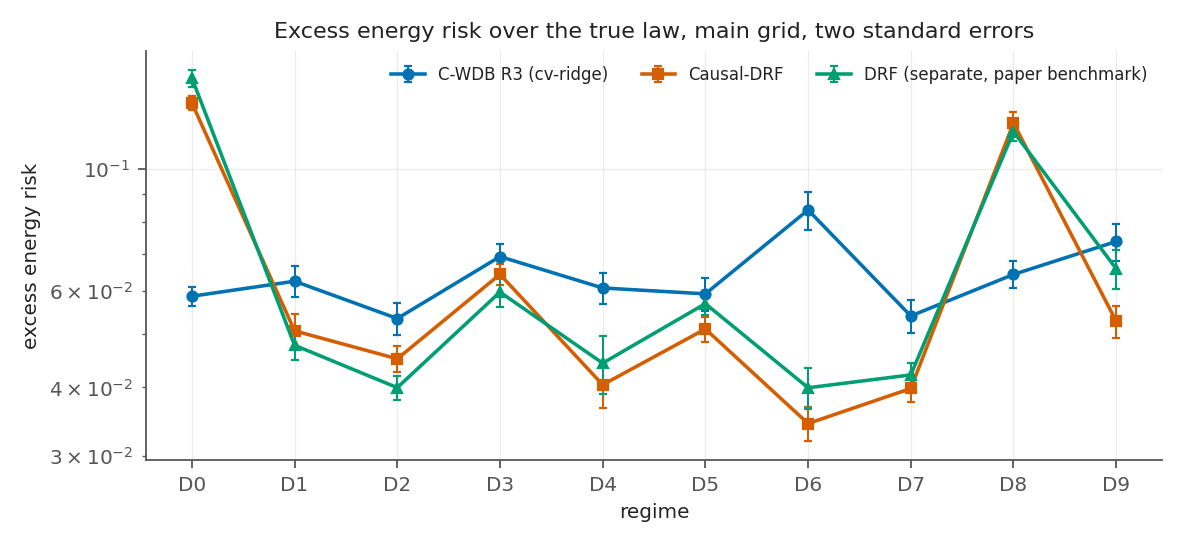
\includegraphics[width=0.94\textwidth]{figures_generated/energy_all_regimes.png}
\caption{Excess energy risk over the true conditional law across all ten regimes.
This is the loss the method actually optimises, evaluated against the quadrature
representation of the truth, so it is the most direct measure of how well the
conditional law itself is estimated. Numbers in Table~\ref{tab:all-energy}.}
\label{fig:energyall}
\end{figure}

\begin{figure}[htbp]
\centering
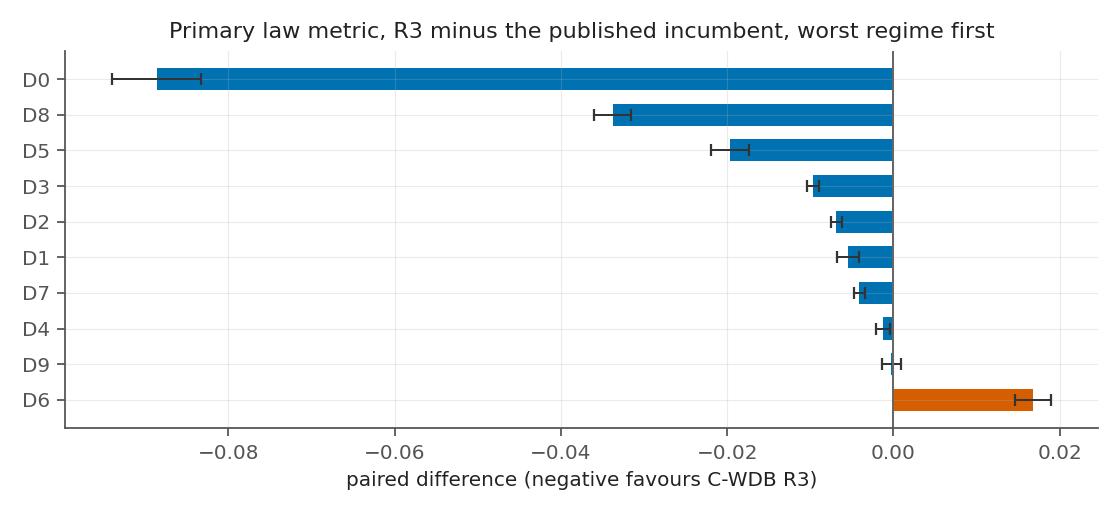
\includegraphics[width=0.9\textwidth]{figures_generated/paired_r3_vs_drf.png}
\caption{The proposed C-WDB R3 against the original-code Causal-DRF comparator
on the primary law metric, worst regime first. Negative values favour R3. This
is the figure behind Table~\ref{tab:paired-r3}.}
\label{fig:pairedr3drf}
\end{figure}

\begin{figure}[htbp]
\centering
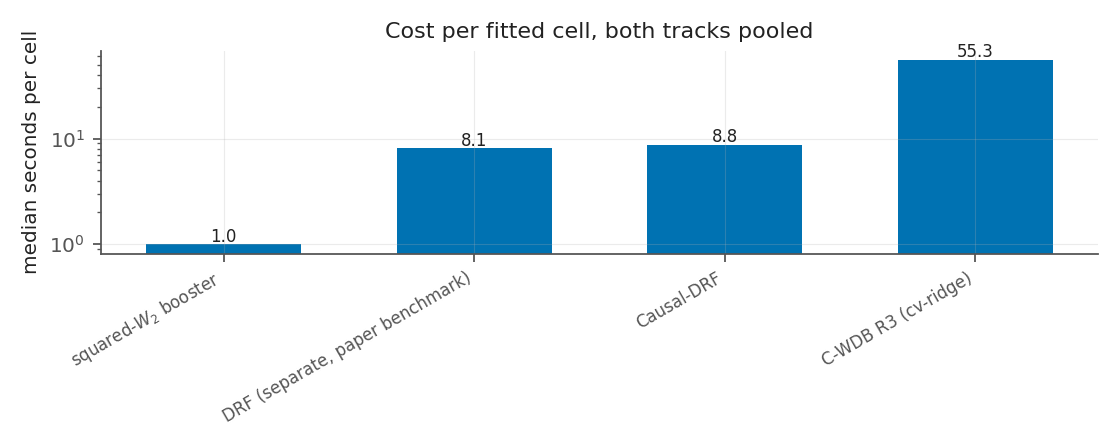
\includegraphics[width=0.94\textwidth]{figures_generated/cost_all_methods.png}
\caption{Median seconds per fitted cell, both tracks pooled, on a logarithmic
axis. The cross-fitted selector is what separates R3 from the other repair
variants: it fits roughly four models where they fit one. Numbers in
Table~\ref{tab:cost-all}.}
\label{fig:costall}
\end{figure}

\clearpage
\section{Complete results: the Phase 5.5 orthogonalized variants}
\label{sec:complete55}

Section~\ref{sec:complete} reports the whole measurement surface for the
proposed model and its comparators on the frozen tournament coordinates. This
section does the same job for the three orthogonalized variants introduced in
Phase 5.5, which were screened on their own manifest and therefore cannot be
appended as extra columns to the tables above without silently changing what a
column means. Every number here is generated from the audited result files by
\texttt{report/build\_phase55\_assets.py} for the Stage 1 screen and by
\texttt{report/build\_phase55\_stage2\_assets.py} for Stage 2, both of which
read and aggregate but never fit a model, exactly as their companion does.

The three variants replace one component of the estimator and leave the rest of
the pipeline frozen. \texttt{cwdb\_rmean} is a vector R-learner in the sense of
Nie and Wager: it fits the causal contrast by minimising the R-loss
$n^{-1}\sum_i \lVert Z_i - \hat m_{-i}(X_i) - (A_i - \hat e_{-i}(X_i))\,t(X_i)
\rVert^2$ over the rescaled quantile coordinates, with exact weighted
least-squares leaves that never divide by $A - \hat e$. \texttt{cwdb\_mutau} is
the Bayesian-causal-forest reparameterisation of the arm-shared tree, carrying a
prognostic field and a contrast field in each leaf through $z_{a,m}(x) = b_m(x)
+ (a - \hat e(x))\,d_m(x)$. \texttt{cwdb\_xmean} is a vector X-learner with
out-of-fold imputed pseudo-outcomes. All three draw their propensity and
prognostic nuisances from one cross-fitted stack with a declared clip of
$[0.02, 0.98]$ and a canonical fold plan that is a pure function of the data
rather than of row order.

The contract difference between them is not cosmetic and it governs which
tables a variant may appear in. \texttt{cwdb\_mutau} produces a conditional law
and is therefore scored on every metric in the report. \texttt{cwdb\_rmean} and
\texttt{cwdb\_xmean} target the arm contrast only and produce no law at all, so
their entries in the law tables are \emph{n/a} by construction rather than by
omission, and no reading of those tables should treat a missing law column as a
loss.

\paragraph{Conventions, and where they differ from Section~\ref{sec:complete}.}
Two of them differ and both differences are deliberate. First, every method in
this section, incumbents included, is restricted to seeds 0 through 9, because
the Phase 5.5 manifest declared ten seeds rather than twenty. Pooling a
twenty-seed incumbent mean against a ten-seed claimant mean in one row would
compare two designs, so the incumbent columns here are recomputed on the
claimant's seeds and will not always equal the same cell in
Section~\ref{sec:complete}. Second, only D0, D2, D7 and D8 appear in the Stage 1
tables. The screen was declared as a mechanism test on the four regimes that
isolate one mechanism each, so it never ran D1, D3, D4, D5, D6 or D9, and no
Stage 1 table supports a statement about the variants outside those four
regimes. Subsection~\ref{sub:stage2} lifts that restriction for the one variant
that continued, at twenty seeds and on all ten regimes; it remains in force for
\texttt{cwdb\_rmean} and \texttt{cwdb\_xmean}, which were never run elsewhere.
Otherwise the conventions carry over: an entry is a mean over cells with the
standard error in parentheses, a cell is one (grid, regime, $n$, $K$, $M$,
method, seed) combination with arm-specific rows averaged inside the cell first,
bold marks the best method in a regime, and a regime mean pools $n = 500$ and
$n = 1000$, which is why the numbers here are not identical to the per-$n$
figures quoted in the G3.5 screen memo. The Causal-DRF and DRF columns are the
original-code reruns, matching the corrected comparator record of
Section~\ref{sec:complete} rather than the retired local drivers.

\subsection{The contrast surface}

Table~\ref{tab:p55-meanq} is the primary table of this section, because
\texttt{mean\_quantile\_rmse} against \texttt{MEANQ-A-K} is the one metric all
seven methods produce. Four readings are worth stating, and the fourth is the
one the screen memo initially failed to make.

The null and deterministic regimes separate the variants sharply. On D2, where
the true effect is exactly zero, \texttt{rmean} records $0.0191$ against
$0.0551$ for PTA-S and $0.0595$ for R3, and Table~\ref{tab:p55-paired-rmean}
shows those gaps are $8.8$ and $3.2$ paired standard errors. This is the
clearest single result of Phase 5.5: orthogonalisation, not more capacity, is
what removes manufactured heterogeneity, and it removes it against the
comparator that motivated the whole repair track. On D8, the confounded regime
that rule 2 of the original gate treated as primary, \texttt{rmean} beats PTA-S
by $2.8$ standard errors but loses to R3 by $5.9$, so the R-loss buys
null-safety at some cost in confounded accuracy.

D7 is where \texttt{rmean} is weakest, at $0.1033$ against $0.0637$ for PTA-S
and $0.0661$ for R3, losing to every comparator in the table by between $2.2$
and $10.9$ standard errors. D7 is the regime whose effect acts through the shape
of the law rather than its location, so a method that estimates the contrast
directly and never represents the law has the least to work with there. That is
a coherent explanation rather than an excuse, and it is also the reason
\texttt{rmean} is recommended as a benchmark rather than as the claimant.

\texttt{cwdb\_mutau} sits close to R3 everywhere and is not interchangeable with
it. Table~\ref{tab:p55-paired-mutau} shows two regimes where the difference
crosses the decision multiple and both go against \texttt{mutau}: D0 by $3.3$
standard errors and D8 by $2.6$. D2 and D7 are ties at $0.4$ and $0.6$. The
honest summary is that the $\mu/\tau$ leaf rule buys nothing against R3 on the
contrast at these sample sizes while costing a little on two regimes, and that
its case rests on the law and functional tables rather than on this one.

\paragraph{The D0 result, stated rather than passed over.} D0 is the regime with
no treatment effect and no confounding, so it is the closest thing in the suite
to a pure bias check. Every C-WDB variant loses it decisively to PTA-S:
$0.0969$ for \texttt{rmean}, $0.0985$ for \texttt{mutau} and $0.0943$ for R3,
against $0.0544$. In paired terms that is $16.0$ standard errors for
\texttt{rmean} and $37.6$ for \texttt{mutau}. The screen memo originally
reported D0 only as passing the $0.15$ correctness cap while reporting the D2
and D8 differences against the same comparator in full, which is a selective
presentation of a comparison that had already been computed. It is corrected
here and in the memo. The deficit is family-wide, not variant-specific, so it is
best read as a property of the boosted particle representation in the regime
where the truth is a single fixed law and the direct learner has nothing to
estimate. It remains an open weakness of the approach, and Stage 2 should report
D0 alongside D2 and D8 as a comparison rather than as a cap check.

Table~\ref{tab:p55-bary} gives the arm-level barycenter error, which is a
different quantity and is never pooled with the contrast. PTA-S is the best
method in all four regimes there, by a wide margin, which is exactly what a
direct arm-level learner should be good at, and the fact that R3 and
\texttt{mutau} nonetheless win contrasts on D8 is the substantive point: the
contrast is not recoverable from arm-level accuracy alone. Tables
\ref{tab:p55-reftcate} and \ref{tab:p55-refate} report the Wasserstein
reference effects, where \texttt{mutau} is best on D7 for both the conditional
and the marginal version and R3 is best on D2 and D8, all by margins smaller
than the ones separating either from the forest comparators.

\subsection{The law surface}

Only \texttt{cwdb\_mutau} enters Tables \ref{tab:p55-kernel} through
\ref{tab:p55-tail}, and the result there is a near-exact tie with R3.
Table~\ref{tab:p55-paired-mutau-law} makes this precise: on
\texttt{kernel\_law\_error} the paired difference against R3 never exceeds
$1.4$ standard errors in any regime, while the difference against Causal-DRF is
a \texttt{mutau} win in all four at between $8.4$ and $23.7$. This is the
expected result and it is a validity check rather than a discovery. The
$\mu/\tau$ parameterisation provably collapses to the reparameterised shared
tree when the propensity basis is the leaf share, a collapse verified in the
test suite to $10^{-14}$ at both the tree and the model level, so a large law
difference against R3 would have indicated a defect rather than a gain.

The functional tables carry the one substantive law-side finding.
Table~\ref{tab:p55-tcate} shows \texttt{mutau} best or tied-best on
\texttt{grid\_mean} and \texttt{grid\_upper\_tail\_mean} in three of four
regimes, and it shows D7 skewness as a failure region for both C-WDB variants:
$0.1134$ for \texttt{mutau} and $0.0860$ for R3 against $0.0514$ for Causal-DRF
and $0.0580$ for DRF, with the same ordering on the marginal version in
Table~\ref{tab:p55-tate}. This is the same documented failure region
Section~\ref{sec:complete} reports for R3 and it is not repaired by the
$\mu/\tau$ leaf rule; if anything \texttt{mutau} is worse there, which is the
$n = 500$ skewness flag recorded in the screen memo. Pure skewness contrasts
remain a region where the forest comparators are better and no claim should be
made over them.

Table~\ref{tab:p55-mode} is a degenerate check in this section, since D6 is not
in the Phase 5.5 manifest and every regime here is single-mode, so the uniform
$1.0000$ column establishes only that nothing broke.

\subsection{The inherited correctness screen}

Table~\ref{tab:p55-rule1} evaluates inherited rule 1 per sample size, under one
convention applied identically to every method: the D2 false-effect ratio
divides a single $n$'s D2 mean by the best frozen baseline at that same $n$.
Pooling the baseline across sample sizes, or mixing a per-$n$ numerator with a
pooled denominator, produces different numbers and appeared in an earlier draft
of the screen memo; it is not the convention and has been removed there too.

The table carries two entries that need reading with care. The first is
\texttt{cwdb\_xmean}, which fails the D0 cap of $0.15$ outright at both sample
sizes, $0.3545$ and $0.3536$. That is the cleanest available statement of its
failure and it is stronger than the comparative statement the screen memo
originally used. The second is R3 at $n = 500$, which shows a D2 ratio of
$1.26$ against a cap of $1.25$. This is an artefact of the ten-seed restriction
and not a new failure: on the full twenty seeds of its own track the same ratio
is $0.98$ at $n = 500$ and $0.93$ pooled, which is what
Section~\ref{sec:complete} reports and what the gate was evaluated on. It is
printed here rather than suppressed because a reader comparing the two sections
would otherwise find the discrepancy unexplained, and because it is a useful
reminder that a threshold evaluated on half the seeds is a different test.

\subsection{The negative finding, and why it is a mechanism result}

\texttt{cwdb\_xmean} exists to test one hypothesis: that out-of-fold imputation
of the missing potential outcome helps when the arms are unbalanced. That
hypothesis is specific to the imbalance regime, so a result outside it could not
support the method, which is why the \texttt{imbalance} extension grid was
declared before the run. Table~\ref{tab:p55-imbalance} reports it. At a realised
mean propensity of $0.307$, \texttt{xmean} wins D7-imb by $9.9$ paired standard
errors, loses D2-imb by $8.0$, and on D8-imb is behind by $1.9$, which does not
cross the decision multiple. One win in the regime the method was built for,
paid for with a large loss on the null, is not a result that continues to
Stage 2.

The verdict was reached on that table alone. Table~\ref{tab:p55-budget} then
answers a separate question, namely whether the failure is a property of the
mechanism or of the frozen three-step effect budget, and it is included here
because the two answers imply different Stage 2 decisions and the difference
must not be settled by assertion. Two observations settle it. The D0 error is
flat in $n$, $0.3545$ against $0.3536$, which no variance story predicts and an
underfit does; and relaxing the budget from three trees to fifty drops D0 from
$0.3550$ to $0.0658$ while D2 rises from $0.0546$ to $0.1636$ and D8 from
$0.1112$ to $0.2222$ over the very same sweep. So the D0 wall is a bias floor
imposed by a total boosting weight of $0.36$ against the R-loss contrast's
$2.4$, and no budget on the sweep is simultaneously effect-recovering and
null-safe. On the imbalance grid the best available budget is the frozen one and
it still loses D2-imb and D8-imb to \texttt{rmean}. The negative finding is
therefore about the mechanism and survives the objection that the budget was
simply miscalibrated. The structural reason is visible in
Table~\ref{tab:p55-diagnostics}: \texttt{rmean} selects its contrast ridge per
cell by cross-fitted selection, choosing $0$ on D0 and between $50$ and $500$
on the regimes with signal, whereas the X pseudo-outcome regression has only a
global constant and no adaptive regulariser at all.

\subsection{Diagnostics and cost}
\label{sub:p55cost}

Table~\ref{tab:p55-diagnostics} collects the quantities only the Phase 5.5
variants emit. Two entries carry weight. The effective particle support is
$10$ of $10$ in every regime for \texttt{mutau}, against a rule-5 floor of
$0.6M = 6$, so the $\mu/\tau$ leaf rule does not collapse the particle cloud.
The selected ridge is $0$ on D0 for both \texttt{rmean} and \texttt{mutau} and
rises to between $250$ and $430$ on the regimes carrying signal, which is the
adaptive behaviour the negative finding above turns on.

Table~\ref{tab:p55-cost} reports runtime with two ratios rather than one,
because the rule-6 verdict for \texttt{mutau} depends entirely on which
Causal-DRF is the denominator and the project contains two. Against the
original-code rerun on exactly these cells, a median of $14.47$ seconds, the
\texttt{mutau} ratio is $11.8$ and comfortably inside the cap of $60$. Against
the retired local driver at $1.87$ seconds, the ratio is $91.1$ and breaches it.
The $91\times$ figure quoted in the screen memo is the second of these. The
first is the denominator the rest of this report uses, so the defensible
statement is that \texttt{mutau} passes rule 6 against the current comparator
record while remaining the most expensive method in the roster at roughly twice
R3 and twelve times Causal-DRF. Two caveats apply to every row. All Phase 5.5
cells ran on a loaded machine alongside other work, so these are upper bounds
rather than clean measurements; and \texttt{mutau} performs a fully nested
refit for its contrast selection while \texttt{rmean} performs a
nested-approximate one that reuses a single nuisance stack, so the eight-second
median of \texttt{rmean} and the one hundred and seventy second median of
\texttt{mutau} are not measurements of the same procedure.

\subsection{Stage 2: the \texorpdfstring{$\mu/\tau$}{mu/tau} claimant on the whole grid}
\label{sub:stage2}

Everything above is the Stage 1 mechanism screen. Phase 5.5 was declared as a
two-stage design in which the screen decides whether a variant addresses its
intended mechanism and Stage 2 is the frozen comparison against the full
tournament record. Only \texttt{cwdb\_mutau} reached it: \texttt{cwdb\_rmean}
cannot supply a law target by contract and was retained as a benchmark rather
than as a claimant, and \texttt{cwdb\_xmean} failed its screen. Stage 2 runs the
claimant on all ten regimes at the twenty seeds every incumbent already carries,
which is $320$ new cells (the six regimes the screen omitted at twenty seeds,
and a seed top-up on the four it ran at ten). The merge audit returned
\textsc{pass} with $320$ of $320$ cells observed, no duplicate keys and no
failures, against manifest checksum
\texttt{29d7ca09\allowbreak 28aa5420\allowbreak 23a091fd\allowbreak 2ffa3943}.

The stage exists because the screen left the phase's own requirement for this
variant unsatisfied. That requirement names D2, D3, D5, D6, D7, D8 and D9, and
the phase's decision table contains the row stating that a candidate which fixes
D2 by losing D3 or D7 is rejected as the main claimant. D3, D5, D6 and D9 had
never been run for this method, so the missing evidence was exactly the evidence
that could overturn the Stage 1 verdict. Thresholds were frozen in
\texttt{research/simulation\_preregistration\_phase55\_stage2.md} before the
first Stage 2 cell was executed, including a numerical definition of the phase
document's word ``materially'' (a paired \texttt{kernel\_law\_error} loss to R3
crossing two standard errors on D3 or D7) and a declaration of which Causal-DRF
record is the rule 6 denominator, since the ambiguity described in
Subsection~\ref{sub:p55cost} would otherwise have recurred.

\paragraph{Two measurement caveats, both settled before the tables were read.}
The first is that \texttt{mutau}'s implementation was modified after the Stage 1
shards were written, during the adversarial audit of the screen memo, and the
source tree is not under version control, so the change could not be diffed. It
was tested instead, by rerunning three cells at coordinates Stage 1 also ran.
Every accuracy quantity reproduced inside the Stage 1 spread while runtime fell
by a factor near five, so the change is a performance change and the two stages
pool on accuracy but not on cost. A subsequent check across all four shared
regimes and four metrics found no difference between the stages at the five
percent level in sixteen comparisons. Accordingly the accuracy tables pool both
stages and every runtime figure is read from Stage 2 rows alone. The second is
that the pooled paired comparisons in the analysis library keyed their per-cell
values by seed alone, so a comparison pooling both sample sizes silently
overwrote one with the other and used half its design points, with the surviving
half determined by dictionary order rather than by the design. This was found
while reconciling the payload against the generated tables, has been corrected
to key on the full design point, and every number in this subsection is
post-correction. Comparisons restricted to a single sample size were never
affected, which includes the Stage 1 tables above.

\paragraph{The gate.} Table~\ref{tab:p55s2-gate} states each preregistered rule
and what it returned. Rules 1 through 6 all pass. Rule 1 clears both caps with
room, at D0 means of $0.1061$ and $0.0894$ against a cap of $0.15$ and D2
false-effect ratios of $0.88$ and $0.69$ against a cap of $1.25$. Rule 5 passes
with the effective particle support at $10$ of $10$ in every regime against a
floor of six, and with D6 mode coverage at $0.9930$, which is the first
measurement of multimodal behaviour for this variant and is the check the screen
could not perform because D6 was not in its manifest. Rule 6 passes at a ratio
of $13.9$ against a cap of $60$.

\paragraph{The law surface.} Tables~\ref{tab:p55s2-kernel}
through~\ref{tab:p55s2-tail} give the law metrics on all ten regimes and
Table~\ref{tab:p55s2-paired-law} gives the paired differences. Rule 2 passes
comfortably: on \texttt{kernel\_law\_error} \texttt{mutau} beats Causal-DRF in
eight regimes against a requirement of two, ties D9, and loses only D6, where
Causal-DRF records $0.0077$ against \texttt{mutau}'s $0.0244$, a loss of $16.1$
paired standard errors. That D6 deficit is the same multimodality weakness
Section~\ref{sec:complete} documents for the C-WDB family and it is not repaired
by the $\mu/\tau$ leaf rule.

Against C-WDB R3 the law result is a tie in seven regimes of ten and a loss in
three, D3 at $3.1$ standard errors, D5 at $2.4$ and D4 at $2.2$, with no regime
in which \texttt{mutau} is better. The Stage 1 conclusion that the two are
near-indistinguishable on the law therefore survives the widening in most
regimes but not everywhere, and where it breaks it breaks against the claimant.
Against C-WDB V1 the picture is genuinely mixed, with \texttt{mutau} better on
D2, D6, D7 and D8 and worse on D0, D1, D4, D5 and D9, which is the expected
signature of a reparameterisation that helps where the contrast is small
relative to the prognostic surface and costs where it is not.

\paragraph{The contrast surface and the accuracy clause.}
Table~\ref{tab:p55s2-meanq} and Table~\ref{tab:p55s2-paired-meanq} carry the
common contrast target. Against R3, \texttt{mutau} loses D0, D3, D4 and D8 by
between $2.3$ and $3.6$ standard errors, wins D5 by $3.1$, and ties the other
five, so the Stage 1 reading that the $\mu/\tau$ leaf rule buys nothing against
R3 on the contrast holds on the wider grid. Against PTA-S it wins D2, D3 and D8
and loses D0, D1, D4, D5 and D6, with the D0 loss at $55.9$ standard errors,
which is the family-wide D0 weakness recorded above at its most extreme.

The accuracy clause is the one place where Stage 2 improves materially on the
original tournament. That clause, frozen before decisive execution, requires a
full-law candidate to win at least one target that PTA-S also estimates, because
the G3 memo recorded rule 4 passing on three capability wins and \emph{zero}
accuracy wins. \texttt{mutau} returns seventeen accuracy wins spread over seven
regimes (D1, D2, D3, D4, D6, D8 and D9), including the marginal functional on
D6 by $5.9$ standard errors and every reference target on D8. This is a real
gain over the incumbent claimant and it is the strongest argument the variant
has.

\paragraph{The degradation clause, which fails.} Table~\ref{tab:p55s2-degradation}
reports it. On D3, the separate-head-favourable regime that a shared prognostic
and contrast tree puts at risk, \texttt{mutau} loses the law metric to R3 at
$n = 500$ by $3.0$ paired standard errors, and the loss shrinks to $1.3$ at
$n = 1000$. D7 is a tie at both sample sizes, so the pure-shape-transfer half of
the clause is satisfied and the sharing half is not. Under the phase's own
decision table this is the row reading that a candidate which fixes D2 while
losing D3 is rejected as the main claimant and its regularisation tradeoff is
reported instead. The magnitude is small in absolute terms, $0.00078$ against a
level near $0.02$, and it is confined to the smaller sample size; the
preregistration nonetheless defined the clause in standard errors rather than in
absolute terms, before the number existed, and the honest reading is that the
clause fails as written rather than that the threshold should now be
reinterpreted.

\paragraph{Diagnostics and cost.} Table~\ref{tab:p55s2-diagnostics} shows the
effective support at the full ten particles in every regime and the selected
contrast strength moving with the signal, at zero on D0 and D2 and rising on the
regimes that carry an effect, which is the adaptive behaviour the mechanism
depends on. Table~\ref{tab:p55s2-cost} puts the \texttt{mutau} median at
$199.3$ seconds against the original-code Causal-DRF's $14.36$, a ratio of
$13.9$. Every figure there is an upper bound: the Stage 2 cells ran sixteen at a
time on one laptop, and the same implementation on an idle machine finishes a
cell in roughly a fifth of the time. Runtime in this project is dominated by
machine load, so the cost rows order the methods reliably and measure none of
them precisely.

\subsection{What this section supports}

Four statements, and no more than four. First, \texttt{cwdb\_rmean} is a
credible null-safe benchmark: it is the best method in the suite on the null
regime by a wide margin, it beats PTA-S on the confounded regime, and it is
cheap, but it loses D0 and D7 badly enough that it is a benchmark and not a
claimant. Second, \texttt{cwdb\_xmean} is a negative finding on the mechanism,
not a tuning failure, and it produced no Stage 2 manifest.

Third, on the evidence of Stage 2, \texttt{cwdb\_mutau} is a real improvement on
the incumbent claimant in one specific respect and not a replacement for it. The
improvement is the accuracy clause: seventeen wins against PTA-S on targets
PTA-S also estimates, spread over seven regimes, where the original tournament
recorded rule 4 passing on capability wins alone. Alongside it the variant
clears every inherited gate rule, beats Causal-DRF on the law metric in eight
regimes of ten, holds full particle support, and is the first C-WDB variant
measured on D6 multimodality, at a mode coverage of $0.9930$. Against that, it
is never better than R3 on the law metric in any regime and is worse in three,
it loses the common contrast to R3 in four regimes and wins one, and it fails
the preregistered degradation clause on D3 at $n = 500$, which is the row the
phase's decision table maps to rejection as the main claimant. The defensible
position is therefore that the $\mu/\tau$ reparameterisation is a reportable
regularisation tradeoff and a candidate complementary estimator, and that
nothing here licenses replacing R3 with it.

Fourth, the scope limits. The Stage 1 tables speak only to D0, D2, D7 and D8,
and nothing in this section speaks to \texttt{cwdb\_rmean} or
\texttt{cwdb\_xmean} outside those four regimes. Stage 2 covers all ten regimes
for \texttt{cwdb\_mutau} alone. No part of this section speaks to any sample
size other than $500$ and $1000$, to any grid resolution other than $K = 25$, to
any particle count other than $M = 10$, or to uncertainty coverage for any
variant, since none has an interval construction and the estimand contract
forbids substituting a posterior-draw quantity.

\begin{table}[htbp]
\centering
\caption{Grid causal mean error \texttt{mean\_quantile\_rmse} against \texttt{MEANQ-A-K}, main grid, mean over 20 cells ($n\in\{500,1000\}$, ten seeds) with the standard error in parentheses. This is the primary contrast metric and the one every Phase 5.5 variant was screened on.}
\label{tab:p55-meanq}
\scriptsize
\setlength{\tabcolsep}{3.2pt}
\begin{tabular}{@{}lrrrrrrr@{}}
\toprule
Regime & rmean & mutau & xmean & R3 & PTA-S & C-DRF & DRF \\
\midrule
D0 & 0.0969\,(0.0038) & 0.0985\,(0.0022) & 0.3540\,(0.0012) & 0.0943\,(0.0021) & \textbf{0.0544\,(0.0018)} & 0.1637\,(0.0059) & 0.1920\,(0.0061) \\
D2 & \textbf{0.0191\,(0.0030)} & 0.0532\,(0.0098) & 0.0473\,(0.0024) & 0.0595\,(0.0116) & 0.0551\,(0.0039) & 0.0952\,(0.0070) & 0.0743\,(0.0064) \\
D7 & 0.1033\,(0.0040) & 0.0647\,(0.0028) & \textbf{0.0624\,(0.0019)} & 0.0661\,(0.0034) & 0.0637\,(0.0035) & 0.0871\,(0.0066) & 0.0787\,(0.0066) \\
D8 & 0.0885\,(0.0025) & 0.0795\,(0.0031) & 0.0915\,(0.0048) & \textbf{0.0739\,(0.0034)} & 0.0984\,(0.0047) & 0.2513\,(0.0137) & 0.1843\,(0.0084) \\
\bottomrule
\end{tabular}
\end{table}

\begin{table}[htbp]
\centering
\caption{Arm-level barycenter error \texttt{barycenter\_rmse}, main grid. This is an arm-level quantity, never pooled with the contrast of Table~\ref{tab:p55-meanq}.}
\label{tab:p55-bary}
\scriptsize
\setlength{\tabcolsep}{3.2pt}
\begin{tabular}{@{}lrrrrrrr@{}}
\toprule
Regime & rmean & mutau & xmean & R3 & PTA-S & C-DRF & DRF \\
\midrule
D0 & 0.1252\,(0.0028) & 0.1077\,(0.0027) & 0.2605\,(0.0013) & 0.1065\,(0.0026) & \textbf{0.0544\,(0.0019)} & 0.2115\,(0.0055) & 0.2321\,(0.0058) \\
D2 & 0.1490\,(0.0019) & 0.1884\,(0.0053) & 0.1653\,(0.0037) & 0.1908\,(0.0053) & \textbf{0.1294\,(0.0032)} & 0.2509\,(0.0060) & 0.2322\,(0.0047) \\
D7 & 0.1482\,(0.0029) & 0.1892\,(0.0050) & 0.1639\,(0.0041) & 0.1892\,(0.0049) & \textbf{0.1306\,(0.0033)} & 0.2294\,(0.0056) & 0.2375\,(0.0050) \\
D8 & 0.3034\,(0.0030) & 0.2540\,(0.0056) & 0.3285\,(0.0062) & 0.2529\,(0.0061) & \textbf{0.1950\,(0.0054)} & 0.4529\,(0.0105) & 0.4436\,(0.0080) \\
\bottomrule
\end{tabular}
\end{table}

\begin{table}[htbp]
\centering
\caption{Declared primary law metric \texttt{kernel\_law\_error} (squared MMD to the true conditional law), main grid. Only \texttt{mutau} produces a law among the Phase 5.5 variants; \texttt{rmean} and \texttt{xmean} target the contrast only and are absent by construction, not by omission.}
\label{tab:p55-kernel}
\scriptsize
\setlength{\tabcolsep}{3.2pt}
\begin{tabular}{@{}lrrrr@{}}
\toprule
Regime & mutau & R3 & C-DRF & DRF \\
\midrule
D0 & 0.0289\,(0.0016) & \textbf{0.0287\,(0.0017)} & 0.1209\,(0.0050) & 0.1422\,(0.0062) \\
D2 & \textbf{0.0117\,(0.0006)} & 0.0122\,(0.0006) & 0.0188\,(0.0008) & 0.0163\,(0.0006) \\
D7 & 0.0118\,(0.0006) & \textbf{0.0117\,(0.0006)} & 0.0159\,(0.0008) & 0.0170\,(0.0007) \\
D8 & 0.0157\,(0.0007) & \textbf{0.0155\,(0.0007)} & 0.0498\,(0.0021) & 0.0483\,(0.0018) \\
\bottomrule
\end{tabular}
\end{table}

\begin{table}[htbp]
\centering
\caption{Excess energy risk over the true conditional law \texttt{arm\_energy\_risk}, main grid. This is the loss the law methods actually optimise.}
\label{tab:p55-energy}
\scriptsize
\setlength{\tabcolsep}{3.2pt}
\begin{tabular}{@{}lrrrr@{}}
\toprule
Regime & mutau & R3 & C-DRF & DRF \\
\midrule
D0 & 0.0584\,(0.0016) & \textbf{0.0579\,(0.0016)} & 0.1312\,(0.0028) & 0.1458\,(0.0037) \\
D2 & 0.0536\,(0.0026) & 0.0551\,(0.0026) & 0.0456\,(0.0018) & \textbf{0.0407\,(0.0014)} \\
D7 & 0.0545\,(0.0026) & 0.0549\,(0.0026) & \textbf{0.0403\,(0.0016)} & 0.0430\,(0.0015) \\
D8 & 0.0650\,(0.0026) & \textbf{0.0644\,(0.0026)} & 0.1213\,(0.0043) & 0.1187\,(0.0037) \\
\bottomrule
\end{tabular}
\end{table}

\begin{table}[htbp]
\centering
\caption{\texttt{mode\_coverage}, the fraction of true outer modes carrying predicted mass, main grid. Higher is better. D6, the only multimodal regime, is not in the Phase 5.5 manifest, so every row here is a degenerate single-mode check.}
\label{tab:p55-mode}
\scriptsize
\setlength{\tabcolsep}{3.2pt}
\begin{tabular}{@{}lrrrr@{}}
\toprule
Regime & mutau & R3 & C-DRF & DRF \\
\midrule
D0 & \textbf{1.0000\,(0.0000)} & \textbf{1.0000\,(0.0000)} & \textbf{1.0000\,(0.0000)} & \textbf{1.0000\,(0.0000)} \\
D2 & \textbf{1.0000\,(0.0000)} & \textbf{1.0000\,(0.0000)} & \textbf{1.0000\,(0.0000)} & \textbf{1.0000\,(0.0000)} \\
D7 & \textbf{1.0000\,(0.0000)} & \textbf{1.0000\,(0.0000)} & \textbf{1.0000\,(0.0000)} & \textbf{1.0000\,(0.0000)} \\
D8 & \textbf{1.0000\,(0.0000)} & \textbf{1.0000\,(0.0000)} & \textbf{1.0000\,(0.0000)} & \textbf{1.0000\,(0.0000)} \\
\bottomrule
\end{tabular}
\end{table}

\begin{table}[htbp]
\centering
\caption{\texttt{tail\_calibration}, absolute error of a predeclared threshold event under the grid law, main grid.}
\label{tab:p55-tail}
\scriptsize
\setlength{\tabcolsep}{3.2pt}
\begin{tabular}{@{}lrrrr@{}}
\toprule
Regime & mutau & R3 & C-DRF & DRF \\
\midrule
D0 & 0.0701\,(0.0019) & \textbf{0.0691\,(0.0023)} & 0.1794\,(0.0045) & 0.1816\,(0.0058) \\
D2 & 0.1165\,(0.0033) & 0.1165\,(0.0034) & 0.1037\,(0.0024) & \textbf{0.0962\,(0.0024)} \\
D7 & 0.0533\,(0.0017) & 0.0534\,(0.0017) & \textbf{0.0433\,(0.0016)} & 0.0442\,(0.0017) \\
D8 & \textbf{0.0988\,(0.0034)} & 0.1002\,(0.0032) & 0.1451\,(0.0041) & 0.1337\,(0.0039) \\
\bottomrule
\end{tabular}
\end{table}

\begin{table}[htbp]
\centering
\caption{Conditional Wasserstein reference effect \texttt{REF-TCATE-K} with $\nu_\star$ the standard normal, main grid.}
\label{tab:p55-reftcate}
\scriptsize
\setlength{\tabcolsep}{3.2pt}
\begin{tabular}{@{}lrrrrrrr@{}}
\toprule
Regime & rmean & mutau & xmean & R3 & PTA-S & C-DRF & DRF \\
\midrule
D0 & n/a & 0.0550\,(0.0019) & n/a & 0.0496\,(0.0017) & \textbf{0.0174\,(0.0019)} & 0.1033\,(0.0039) & 0.1113\,(0.0077) \\
D2 & n/a & 0.0202\,(0.0035) & n/a & \textbf{0.0184\,(0.0030)} & 0.0235\,(0.0043) & 0.0287\,(0.0045) & 0.0301\,(0.0045) \\
D7 & n/a & \textbf{0.0215\,(0.0027)} & n/a & 0.0232\,(0.0028) & 0.0244\,(0.0035) & 0.0294\,(0.0036) & 0.0296\,(0.0036) \\
D8 & n/a & \textbf{0.0426\,(0.0038)} & n/a & 0.0444\,(0.0036) & 0.0624\,(0.0039) & 0.0695\,(0.0069) & 0.0866\,(0.0080) \\
\bottomrule
\end{tabular}
\end{table}

\begin{table}[htbp]
\centering
\caption{Marginal Wasserstein reference effect \texttt{REF-ATE-K}, main grid.}
\label{tab:p55-refate}
\scriptsize
\setlength{\tabcolsep}{3.2pt}
\begin{tabular}{@{}lrrrrrrr@{}}
\toprule
Regime & rmean & mutau & xmean & R3 & PTA-S & C-DRF & DRF \\
\midrule
D0 & n/a & 0.0436\,(0.0016) & n/a & 0.0385\,(0.0014) & \textbf{0.0047\,(0.0009)} & 0.0129\,(0.0025) & 0.0102\,(0.0031) \\
D2 & n/a & 0.0123\,(0.0036) & n/a & \textbf{0.0096\,(0.0026)} & 0.0169\,(0.0047) & 0.0195\,(0.0051) & 0.0182\,(0.0046) \\
D7 & n/a & \textbf{0.0140\,(0.0029)} & n/a & 0.0150\,(0.0033) & 0.0158\,(0.0040) & 0.0174\,(0.0044) & 0.0167\,(0.0039) \\
D8 & n/a & 0.0239\,(0.0033) & n/a & \textbf{0.0238\,(0.0028)} & 0.0412\,(0.0057) & 0.0491\,(0.0081) & 0.0667\,(0.0101) \\
\bottomrule
\end{tabular}
\end{table}

\begin{table}[htbp]
\centering
\caption{Conditional functional treatment effects \texttt{tcate\_functional\_rmse}, main grid. D7 is the transfer regime the law claim rests on.}
\label{tab:p55-tcate}
\scriptsize
\setlength{\tabcolsep}{3.2pt}
\begin{tabular}{@{}llrrrr@{}}
\toprule
Functional & Regime & mutau & R3 & C-DRF & DRF \\
\midrule
\texttt{grid\_mean} & D0 & 0.0606\,(0.0019) & \textbf{0.0555\,(0.0019)} & 0.1166\,(0.0058) & 0.1093\,(0.0087) \\
 & D2 & \textbf{0.0268\,(0.0042)} & 0.0274\,(0.0043) & 0.0741\,(0.0087) & 0.0527\,(0.0082) \\
 & D7 & \textbf{0.0244\,(0.0032)} & 0.0295\,(0.0040) & 0.0608\,(0.0084) & 0.0535\,(0.0086) \\
 & D8 & \textbf{0.0573\,(0.0049)} & 0.0586\,(0.0037) & 0.2117\,(0.0165) & 0.1306\,(0.0125) \\
\midrule
\texttt{grid\_sd} & D0 & 0.0117\,(0.0009) & \textbf{0.0101\,(0.0008)} & 0.0171\,(0.0014) & 0.0168\,(0.0015) \\
 & D2 & \textbf{0.0169\,(0.0021)} & 0.0173\,(0.0019) & 0.0180\,(0.0022) & 0.0182\,(0.0020) \\
 & D7 & 0.0183\,(0.0016) & 0.0182\,(0.0021) & 0.0198\,(0.0024) & \textbf{0.0182\,(0.0020)} \\
 & D8 & 0.0204\,(0.0022) & \textbf{0.0173\,(0.0022)} & 0.0267\,(0.0021) & 0.0238\,(0.0021) \\
\midrule
\texttt{grid\_skewness} & D0 & 0.0124\,(0.0023) & 0.0120\,(0.0023) & \textbf{0.0000\,(0.0000)} & 0.0000\,(0.0000) \\
 & D2 & 0.0000\,(0.0000) & 0.0000\,(0.0000) & 0.0000\,(0.0000) & \textbf{0.0000\,(0.0000)} \\
 & D7 & 0.1134\,(0.0140) & 0.0860\,(0.0068) & \textbf{0.0514\,(0.0032)} & 0.0580\,(0.0026) \\
 & D8 & 0.0000\,(0.0000) & 0.0000\,(0.0000) & 0.0000\,(0.0000) & \textbf{0.0000\,(0.0000)} \\
\midrule
\texttt{grid\_upper\_tail\_mean} & D0 & 0.0603\,(0.0019) & \textbf{0.0551\,(0.0018)} & 0.1223\,(0.0063) & 0.1129\,(0.0089) \\
 & D2 & \textbf{0.0308\,(0.0040)} & 0.0311\,(0.0045) & 0.0784\,(0.0089) & 0.0567\,(0.0085) \\
 & D7 & \textbf{0.0291\,(0.0033)} & 0.0330\,(0.0038) & 0.0643\,(0.0084) & 0.0572\,(0.0088) \\
 & D8 & 0.0608\,(0.0050) & \textbf{0.0596\,(0.0039)} & 0.2207\,(0.0169) & 0.1361\,(0.0124) \\
\bottomrule
\end{tabular}
\end{table}

\begin{table}[htbp]
\centering
\caption{Marginal functional treatment effects \texttt{tate\_functional\_rmse}, main grid.}
\label{tab:p55-tate}
\scriptsize
\setlength{\tabcolsep}{3.2pt}
\begin{tabular}{@{}llrrrr@{}}
\toprule
Functional & Regime & mutau & R3 & C-DRF & DRF \\
\midrule
\texttt{grid\_mean} & D0 & 0.0064\,(0.0011) & \textbf{0.0052\,(0.0011)} & 0.0575\,(0.0060) & 0.0312\,(0.0048) \\
 & D2 & \textbf{0.0158\,(0.0024)} & 0.0177\,(0.0029) & 0.0657\,(0.0088) & 0.0255\,(0.0056) \\
 & D7 & \textbf{0.0163\,(0.0027)} & 0.0178\,(0.0027) & 0.0462\,(0.0086) & 0.0263\,(0.0057) \\
 & D8 & \textbf{0.0318\,(0.0054)} & 0.0369\,(0.0048) & 0.1850\,(0.0197) & 0.0714\,(0.0136) \\
\midrule
\texttt{grid\_sd} & D0 & 0.0057\,(0.0010) & \textbf{0.0042\,(0.0009)} & 0.0138\,(0.0017) & 0.0132\,(0.0017) \\
 & D2 & \textbf{0.0119\,(0.0021)} & 0.0121\,(0.0017) & 0.0142\,(0.0024) & 0.0137\,(0.0023) \\
 & D7 & \textbf{0.0118\,(0.0014)} & 0.0124\,(0.0019) & 0.0143\,(0.0026) & 0.0136\,(0.0023) \\
 & D8 & 0.0137\,(0.0019) & \textbf{0.0121\,(0.0023)} & 0.0191\,(0.0022) & 0.0192\,(0.0022) \\
\midrule
\texttt{grid\_skewness} & D0 & 0.0102\,(0.0024) & 0.0106\,(0.0024) & \textbf{0.0000\,(0.0000)} & 0.0000\,(0.0000) \\
 & D2 & 0.0000\,(0.0000) & 0.0000\,(0.0000) & 0.0000\,(0.0000) & \textbf{0.0000\,(0.0000)} \\
 & D7 & 0.0977\,(0.0124) & 0.0704\,(0.0059) & 0.0181\,(0.0026) & \textbf{0.0148\,(0.0023)} \\
 & D8 & 0.0000\,(0.0000) & 0.0000\,(0.0000) & \textbf{0.0000\,(0.0000)} & 0.0000\,(0.0000) \\
\midrule
\texttt{grid\_upper\_tail\_mean} & D0 & 0.0071\,(0.0014) & \textbf{0.0055\,(0.0007)} & 0.0677\,(0.0065) & 0.0400\,(0.0052) \\
 & D2 & 0.0204\,(0.0030) & \textbf{0.0197\,(0.0035)} & 0.0706\,(0.0091) & 0.0301\,(0.0066) \\
 & D7 & \textbf{0.0191\,(0.0037)} & 0.0203\,(0.0036) & 0.0504\,(0.0088) & 0.0301\,(0.0065) \\
 & D8 & \textbf{0.0317\,(0.0059)} & 0.0357\,(0.0050) & 0.1953\,(0.0199) & 0.0820\,(0.0141) \\
\bottomrule
\end{tabular}
\end{table}

\begin{table}[htbp]
\centering
\caption{Inherited rule 1, evaluated per sample size on the ten Phase 5.5 seeds. The D0 cap is 0.15, the D2 cap is 0.15, and the D2 false-effect ratio cap is 1.25 times the best frozen baseline at the same $n$.}
\label{tab:p55-rule1}
\small
\begin{tabular}{@{}llrrrrl@{}}
\toprule
Method & $n$ & D0 & D2 & baseline & ratio & Verdict \\
\midrule
rmean & 500 & 0.1095 & 0.0149 & 0.0620 & 0.24 & \textsc{pass} \\
rmean & 1000 & 0.0842 & 0.0233 & 0.0482 & 0.48 & \textsc{pass} \\
\addlinespace
mutau & 500 & 0.1063 & 0.0714 & 0.0620 & 1.15 & \textsc{pass} \\
mutau & 1000 & 0.0907 & 0.0349 & 0.0482 & 0.72 & \textsc{pass} \\
\addlinespace
xmean & 500 & 0.3545 & 0.0553 & 0.0620 & 0.89 & \textbf{FAIL} \\
xmean & 1000 & 0.3536 & 0.0394 & 0.0482 & 0.82 & \textbf{FAIL} \\
\addlinespace
R3 & 500 & 0.1017 & 0.0780 & 0.0620 & 1.26 & \textbf{FAIL} \\
R3 & 1000 & 0.0868 & 0.0410 & 0.0482 & 0.85 & \textsc{pass} \\
\addlinespace
PTA-S & 500 & 0.0623 & 0.0620 & 0.0620 & 1.00 & \textsc{pass} \\
PTA-S & 1000 & 0.0465 & 0.0482 & 0.0482 & 1.00 & \textsc{pass} \\
\addlinespace
C-DRF & 500 & 0.1883 & 0.1086 & 0.0620 & 1.75 & \textbf{FAIL} \\
C-DRF & 1000 & 0.1391 & 0.0818 & 0.0482 & 1.70 & \textbf{FAIL} \\
\addlinespace
DRF & 500 & 0.2168 & 0.0860 & 0.0620 & 1.39 & \textbf{FAIL} \\
DRF & 1000 & 0.1672 & 0.0627 & 0.0482 & 1.30 & \textbf{FAIL} \\
\bottomrule
\end{tabular}
\par\vspace{2pt}\parbox{0.9\textwidth}{\scriptsize The baseline column is the smallest D2 mean among PTA-S, C-WDB-v0, C-WDB-v1, W-DRF-T and Causal-DRF at that $n$, on the same ten seeds. Causal-DRF and DRF are included as rows for reference; they are incumbents, not claimants, and rule 1 was never a gate on them.}
\end{table}

\begin{table}[htbp]
\centering
\caption{Seed-paired \texttt{mean\_quantile\_rmse} differences for \texttt{cwdb\_rmean}. The D8 column is the primary confounding test and the D0 column is the one the screen memo initially omitted.}
\label{tab:p55-paired-rmean}
\scriptsize
\setlength{\tabcolsep}{4pt}
\begin{tabular}{@{}lrrrrrrrrr@{}}
\toprule
Regime & \multicolumn{3}{c}{vs PTA-S} & \multicolumn{3}{c}{vs R3} & \multicolumn{3}{c}{vs C-DRF} \\
  & diff. & SE & $|$diff$|/$SE & diff. & SE & $|$diff$|/$SE & diff. & SE & $|$diff$|/$SE \\
\midrule
D0 & +0.0425$^{\dagger}$ & 0.0026 & 16.0 & +0.0026 & 0.0033 & 0.8 & -0.0669$^{\ast}$ & 0.0039 & 17.0 \\
D2 & -0.0360$^{\ast}$ & 0.0041 & 8.8 & -0.0404$^{\ast}$ & 0.0127 & 3.2 & -0.0761$^{\ast}$ & 0.0082 & 9.3 \\
D7 & +0.0396$^{\dagger}$ & 0.0036 & 10.9 & +0.0372$^{\dagger}$ & 0.0039 & 9.5 & +0.0163$^{\dagger}$ & 0.0073 & 2.2 \\
D8 & -0.0100$^{\ast}$ & 0.0036 & 2.8 & +0.0145$^{\dagger}$ & 0.0025 & 5.9 & -0.1628$^{\ast}$ & 0.0134 & 12.1 \\
\bottomrule
\end{tabular}
\par\vspace{2pt}\parbox{0.96\textwidth}{\scriptsize Negative favours the claimant. $\ast$ marks a claimant win and $\dagger$ a comparator win, both at more than two paired standard errors, which is the frozen decision multiple. The third column of each block is the same quantity expressed in standard errors, so a reader can see how far past the threshold a result sits rather than only that it crossed.}
\end{table}

\begin{table}[htbp]
\centering
\caption{Seed-paired \texttt{mean\_quantile\_rmse} differences for \texttt{cwdb\_mutau}. The R3 block is the informative one: \texttt{mutau} is a reparameterisation of the same shared tree, so a difference against R3 is a difference the $\mu/\tau$ leaf rule caused.}
\label{tab:p55-paired-mutau}
\scriptsize
\setlength{\tabcolsep}{4pt}
\begin{tabular}{@{}lrrrrrrrrr@{}}
\toprule
Regime & \multicolumn{3}{c}{vs R3} & \multicolumn{3}{c}{vs PTA-S} & \multicolumn{3}{c}{vs C-DRF} \\
  & diff. & SE & $|$diff$|/$SE & diff. & SE & $|$diff$|/$SE & diff. & SE & $|$diff$|/$SE \\
\midrule
D0 & +0.0042$^{\dagger}$ & 0.0013 & 3.3 & +0.0441$^{\dagger}$ & 0.0012 & 37.6 & -0.0652$^{\ast}$ & 0.0045 & 14.5 \\
D2 & -0.0063 & 0.0148 & 0.4 & -0.0019 & 0.0084 & 0.2 & -0.0420$^{\ast}$ & 0.0120 & 3.5 \\
D7 & -0.0015 & 0.0027 & 0.6 & +0.0009 & 0.0024 & 0.4 & -0.0224$^{\ast}$ & 0.0060 & 3.7 \\
D8 & +0.0055$^{\dagger}$ & 0.0022 & 2.6 & -0.0190$^{\ast}$ & 0.0042 & 4.6 & -0.1718$^{\ast}$ & 0.0143 & 12.1 \\
\bottomrule
\end{tabular}
\par\vspace{2pt}\parbox{0.96\textwidth}{\scriptsize Negative favours the claimant. $\ast$ marks a claimant win and $\dagger$ a comparator win, both at more than two paired standard errors, which is the frozen decision multiple. The third column of each block is the same quantity expressed in standard errors, so a reader can see how far past the threshold a result sits rather than only that it crossed.}
\end{table}

\begin{table}[htbp]
\centering
\caption{Seed-paired \texttt{mean\_quantile\_rmse} differences for \texttt{cwdb\_xmean} on the main grid. The imbalance grid, which is where its premise lives, is Table~\ref{tab:p55-imbalance}.}
\label{tab:p55-paired-xmean}
\scriptsize
\setlength{\tabcolsep}{4pt}
\begin{tabular}{@{}lrrrrrrrrr@{}}
\toprule
Regime & \multicolumn{3}{c}{vs rmean} & \multicolumn{3}{c}{vs PTA-S} & \multicolumn{3}{c}{vs R3} \\
  & diff. & SE & $|$diff$|/$SE & diff. & SE & $|$diff$|/$SE & diff. & SE & $|$diff$|/$SE \\
\midrule
D0 & +0.2572$^{\dagger}$ & 0.0037 & 70.3 & +0.2996$^{\dagger}$ & 0.0021 & 140.3 & +0.2597$^{\dagger}$ & 0.0027 & 97.7 \\
D2 & +0.0283$^{\dagger}$ & 0.0042 & 6.7 & -0.0077$^{\ast}$ & 0.0031 & 2.5 & -0.0122 & 0.0118 & 1.0 \\
D7 & -0.0410$^{\ast}$ & 0.0037 & 11.1 & -0.0014 & 0.0029 & 0.5 & -0.0038 & 0.0025 & 1.5 \\
D8 & +0.0031 & 0.0049 & 0.6 & -0.0069 & 0.0056 & 1.2 & +0.0176$^{\dagger}$ & 0.0036 & 4.9 \\
\bottomrule
\end{tabular}
\par\vspace{2pt}\parbox{0.96\textwidth}{\scriptsize Negative favours the claimant. $\ast$ marks a claimant win and $\dagger$ a comparator win, both at more than two paired standard errors, which is the frozen decision multiple. The third column of each block is the same quantity expressed in standard errors, so a reader can see how far past the threshold a result sits rather than only that it crossed.}
\end{table}

\begin{table}[htbp]
\centering
\caption{Seed-paired \texttt{kernel\_law\_error} differences for \texttt{cwdb\_mutau}, the law metric.}
\label{tab:p55-paired-mutau-law}
\scriptsize
\setlength{\tabcolsep}{4pt}
\begin{tabular}{@{}lrrrrrr@{}}
\toprule
Regime & \multicolumn{3}{c}{vs R3} & \multicolumn{3}{c}{vs C-DRF} \\
  & diff. & SE & $|$diff$|/$SE & diff. & SE & $|$diff$|/$SE \\
\midrule
D0 & +0.0001 & 0.0006 & 0.2 & -0.0920$^{\ast}$ & 0.0039 & 23.7 \\
D2 & -0.0005 & 0.0004 & 1.4 & -0.0071$^{\ast}$ & 0.0006 & 11.6 \\
D7 & +0.0000 & 0.0002 & 0.1 & -0.0041$^{\ast}$ & 0.0005 & 8.4 \\
D8 & +0.0003 & 0.0003 & 1.0 & -0.0341$^{\ast}$ & 0.0016 & 21.3 \\
\bottomrule
\end{tabular}
\par\vspace{2pt}\parbox{0.96\textwidth}{\scriptsize Negative favours the claimant. $\ast$ marks a claimant win and $\dagger$ a comparator win, both at more than two paired standard errors, which is the frozen decision multiple. The third column of each block is the same quantity expressed in standard errors, so a reader can see how far past the threshold a result sits rather than only that it crossed.}
\end{table}

\begin{table}[htbp]
\centering
\caption{The \texttt{imbalance} extension grid, $n=500$, ten seeds. This grid was added for WP5.5-D: the vector X-learner's claimed advantage is specific to arm imbalance, so a result outside this grid could not support it. The last two columns are the seed-paired difference of \texttt{xmean} against \texttt{rmean} on \texttt{mean\_quantile\_rmse}.}
\label{tab:p55-imbalance}
\small
\begin{tabular}{@{}lrrrrrr@{}}
\toprule
& \multicolumn{2}{c}{\texttt{mean\_quantile\_rmse}} & \multicolumn{2}{c}{\texttt{barycenter\_rmse}} & \multicolumn{2}{c}{paired diff.} \\
\cmidrule(lr){2-3}\cmidrule(lr){4-5}\cmidrule(lr){6-7}
Regime & rmean & xmean & rmean & xmean & diff. & SE \\
\midrule
D2-imb & 0.0153\,(0.0056) & 0.0706\,(0.0053) & 0.1585\,(0.0028) & 0.1797\,(0.0026) & +0.0553$^{\dagger}$ & 0.0069 \\
D7-imb & 0.1289\,(0.0039) & 0.0833\,(0.0043) & 0.1722\,(0.0030) & 0.1785\,(0.0039) & -0.0456$^{\ast}$ & 0.0046 \\
D8-imb & 0.0911\,(0.0026) & 0.1033\,(0.0054) & 0.2954\,(0.0042) & 0.3103\,(0.0055) & +0.0121 & 0.0064 \\
\bottomrule
\end{tabular}
\par\vspace{2pt}\parbox{0.9\textwidth}{\scriptsize Negative favours \texttt{xmean}; $\dagger$ marks an \texttt{rmean} win beyond two paired standard errors. The imbalance actually realised, as the mean fitted propensity: D2-imb 0.307, D7-imb 0.307, D8-imb 0.307.}
\end{table}

\begin{table}[htbp]
\centering
\caption{Post-decision diagnostic for \texttt{cwdb\_xmean}: \texttt{mean\_quantile\_rmse} as the frozen three-step effect budget is relaxed, five seeds. The frozen budget is the first column. No column is simultaneously effect-recovering and null-safe, and on the imbalance grid the best available column is still the frozen one and still loses to \texttt{rmean}.}
\label{tab:p55-budget}
\small
\begin{tabular}{@{}lrrrrr@{}}
\toprule
Cell & $B=3$ & $B=10$ & $B=20$ & $B=50$ & \texttt{rmean} \\
\midrule
\texttt{D0/n500} & 0.3550 & 0.1669 & 0.0850 & 0.0658 & n/a \\
\texttt{D0/n1000} & 0.3510 & 0.1644 & 0.0767 & 0.0520 & n/a \\
\texttt{D2/n500} & 0.0546 & 0.0925 & 0.1217 & 0.1636 & n/a \\
\texttt{D2/n1000} & 0.0387 & 0.0716 & 0.0958 & 0.1295 & n/a \\
\texttt{D8/n500} & 0.1112 & 0.1472 & 0.1770 & 0.2222 & n/a \\
\texttt{D8/n1000} & 0.0854 & 0.1145 & 0.1446 & 0.1810 & n/a \\
\midrule
\texttt{D2-imb/n500} & 0.0682 & 0.1132 & 0.1499 & 0.1926 & 0.0086 \\
\texttt{D7-imb/n500} & 0.0816 & 0.1181 & 0.1483 & 0.1893 & 0.1305 \\
\texttt{D8-imb/n500} & 0.1017 & 0.1532 & 0.1900 & 0.2338 & 0.0931 \\
\bottomrule
\end{tabular}
\par\vspace{2pt}\parbox{0.9\textwidth}{\scriptsize $B$ is \texttt{n\_estimators} in the effect regression; the learning rate stays at 0.12, so the frozen budget carries total boosting weight 0.36 against the R-loss contrast's 2.4. Generated by \texttt{research/checks/phase55\_xmean\_budget\_probe.py}. This probe explains a verdict already reached and no threshold depends on it.}
\end{table}

\begin{table}[htbp]
\centering
\caption{Mechanism diagnostics recorded by the Phase 5.5 variants, main grid, mean over the twenty cells of a regime with the standard error in parentheses. These are not comparisons: no incumbent emits them.}
\label{tab:p55-diagnostics}
\scriptsize
\setlength{\tabcolsep}{4pt}
\begin{tabular}{@{}llrrrr@{}}
\toprule
Method & Diagnostic & D0 & D2 & D7 & D8 \\
\midrule
rmean & selected ridge $\lambda$ & 0.000\,(0.000) & 432.500\,(36.863) & 50.000\,(0.000) & 297.500\,(51.360) \\
mutau & selected ridge $\lambda$ & 0.000\,(0.000) & 272.500\,(52.249) & 252.500\,(51.360) & 297.500\,(51.360) \\
mutau & boosting steps used & 100.000\,(0.000) & 100.000\,(0.000) & 100.000\,(0.000) & 100.000\,(0.000) \\
mutau & effective particle support & 10.000\,(0.000) & 10.000\,(0.000) & 10.000\,(0.000) & 10.000\,(0.000) \\
xmean & $\bar{\hat e}$ & 0.497\,(0.005) & 0.497\,(0.005) & 0.497\,(0.005) & 0.496\,(0.004) \\
xmean & sd of $\hat e$ & 0.128\,(0.004) & 0.128\,(0.004) & 0.128\,(0.004) & 0.295\,(0.003) \\
rmean & training risk & 0.011\,(0.000) & 0.189\,(0.002) & 0.185\,(0.002) & 0.255\,(0.004) \\
mutau & training risk & 0.023\,(0.000) & 0.130\,(0.006) & 0.131\,(0.006) & 0.158\,(0.005) \\
\bottomrule
\end{tabular}
\par\vspace{2pt}\parbox{0.94\textwidth}{\scriptsize The effective support is the number of the $M=10$ particles carrying non-negligible weight, so 10 is the ceiling and the floor for rule 5 is $0.6M=6$. The selected $\lambda$ is chosen per cell from $\{0, 50, 500\}$ by cross-fitted selection, so its mean is a per-regime average of a discrete choice and not itself a tuned value.}
\end{table}

\begin{table}[htbp]
\centering
\caption{Operational cost on the Phase 5.5 coordinates: every \texttt{main} grid cell of D0, D2, D7 and D8 at ten seeds. Two cost ratios are reported against the inherited cap of 60, because the rule-6 verdict depends on which Causal-DRF is the denominator and the project contains two.}
\label{tab:p55-cost}
\small
\begin{tabular}{@{}lrrrrrrr@{}}
\toprule
Method & Cells & Median (s) & Mean (s) & Max (s) & Ratio$_{\text{orig}}$ & Ratio$_{\text{local}}$ & Median RAM (MB) \\
\midrule
C-WDB rmean (vector R-learner) & 80 & 8.27 & 8.77 & 15.8 & 0.6 & 4.4 & 0 \\
C-WDB mutau ($\mu/\tau$ shared tree) & 80 & 170.19 & 180.68 & 321.4 & 11.8 & 91.1 & 0 \\
C-WDB xmean (vector X-learner) & 80 & 5.03 & 5.40 & 9.8 & 0.3 & 2.7 & 0 \\
C-WDB R3 (cv-ridge) & 80 & 84.47 & 87.11 & 134.0 & 5.8 & 45.2 & 0 \\
PTA-S & 80 & 35.36 & 35.73 & 51.4 & 2.4 & 18.9 & 0 \\
Causal-DRF & 80 & 14.47 & 13.10 & 38.1 & 1.0 & 7.7 & 336 \\
DRF (separate, paper benchmark) & 80 & 11.32 & 10.93 & 33.4 & 0.8 & 6.1 & 431 \\
\bottomrule
\end{tabular}
\par\vspace{2pt}\parbox{0.94\textwidth}{\scriptsize Ratio$_{\text{orig}}$ divides by the original-code Causal-DRF rerun on exactly these cells (median 14.47\,s), which is the comparator record the rest of this report uses. Ratio$_{\text{local}}$ divides by the retired local Causal-DRF driver pooled over its own \texttt{main} grid, all ten regimes (median 1.87\,s), which is the denominator the G3.5 screen memo quoted. Every Phase 5.5 cell ran on a loaded machine alongside other work, so these are upper bounds on the variants' cost rather than clean measurements; the ratios are reported anyway because the cap is a declared gate and a favourable rerun cannot be assumed.}
\end{table}

\begin{table}[htbp]
\centering
\caption{Phase 5.5 Stage 2 against the rules frozen in \texttt{research/simulation\_preregistration\_phase55\_stage2.md} before the first Stage 2 cell was executed. Claimant \texttt{cwdb\_mutau}, ten regimes, twenty seeds.}
\label{tab:p55s2-gate}
\scriptsize
\setlength{\tabcolsep}{4pt}
\begin{tabular}{@{}p{0.30\textwidth}p{0.50\textwidth}l@{}}
\toprule
Rule & Result & Verdict \\
\midrule
Rule 1, correctness and nulls & D0 0.1061 and 0.0894 under 0.15; D2 ratio 0.88 and 0.69 under 1.25 & \textbf{PASS} \\
Rule 2, law advantage over Causal-DRF & 8 regimes of 2 required: D0, D1, D2, D3, D4, D5, D7, D8 & \textbf{PASS} \\
Rules 3 and 4, transfer and direct learner & 25 functional or reference targets won against Causal-DRF; 17 accuracy wins against PTA-S across 7 regimes & \textbf{PASS} \\
Rule 5, no particle collapse & effective support 10.0 of 10 against a floor of 6; D6 mode coverage 0.9930 & \textbf{PASS} \\
Rule 6, cost & median 199.3\,s against 14.36\,s, ratio 13.9 against a cap of 60 & \textbf{PASS} \\
Accuracy clause, at least one win over PTA-S & 17 wins on targets both methods estimate, in D1, D2, D3, D4, D6, D8, D9 & \textbf{PASS} \\
Degradation clause, D3 sharing and D7 shape & D3@n500 crosses the multiple against R3 & \textbf{FAIL} \\
\bottomrule
\end{tabular}
\par\vspace{2pt}\parbox{0.96\textwidth}{\scriptsize Rules 1 through 6 are the inherited G3 gate rules. The last two rows are the clauses the phase document froze specifically for a Stage 2 full-law candidate. The degradation clause was given its numerical definition (a paired \texttt{kernel\_law\_error} loss to R3 crossing two standard errors on D3 or D7) in the preregistration, before the result existed.}
\end{table}

\begin{table}[htbp]
\centering
\caption{Stage 2 grid causal mean: \texttt{mean\_quantile\_rmse} against \texttt{MEANQ-A-K}, every regime, twenty seeds. Mean over cells with the standard error in parentheses; bold marks the best method in a regime.}
\label{tab:p55s2-meanq}
\scriptsize
\setlength{\tabcolsep}{3.2pt}
\begin{tabular}{@{}lrrrrrr@{}}
\toprule
Regime & mutau & R3 & v1 & PTA-S & C-DRF & DRF \\
\midrule
D0 & 0.0977\,(0.0015) & 0.0952\,(0.0016) & 0.1091\,(0.0021) & \textbf{0.0547\,(0.0013)} & 0.1621\,(0.0038) & 0.1935\,(0.0048) \\
D1 & 0.2053\,(0.0044) & 0.2043\,(0.0042) & 0.1899\,(0.0042) & \textbf{0.1427\,(0.0030)} & 0.2119\,(0.0062) & 0.2017\,(0.0049) \\
D2 & \textbf{0.0433\,(0.0054)} & 0.0506\,(0.0063) & 0.1466\,(0.0038) & 0.0545\,(0.0030) & 0.0960\,(0.0046) & 0.0754\,(0.0042) \\
D3 & 0.2896\,(0.0054) & \textbf{0.2861\,(0.0049)} & 0.2891\,(0.0058) & 0.2947\,(0.0058) & 0.4301\,(0.0060) & 0.4088\,(0.0072) \\
D4 & 0.2062\,(0.0053) & 0.2002\,(0.0048) & 0.1979\,(0.0051) & \textbf{0.1372\,(0.0036)} & 0.1603\,(0.0062) & 0.1697\,(0.0078) \\
D5 & 0.1346\,(0.0131) & 0.1644\,(0.0133) & 0.1757\,(0.0037) & \textbf{0.0500\,(0.0031)} & 0.0885\,(0.0038) & 0.1004\,(0.0041) \\
D6 & 0.2530\,(0.0120) & 0.2477\,(0.0108) & 0.2898\,(0.0125) & 0.2320\,(0.0098) & 0.2567\,(0.0128) & \textbf{0.2247\,(0.0129)} \\
D7 & 0.0713\,(0.0056) & 0.0683\,(0.0042) & 0.1460\,(0.0037) & \textbf{0.0636\,(0.0026)} & 0.0870\,(0.0042) & 0.0794\,(0.0043) \\
D8 & 0.0776\,(0.0020) & \textbf{0.0735\,(0.0022)} & 0.1848\,(0.0041) & 0.0950\,(0.0030) & 0.2638\,(0.0104) & 0.1790\,(0.0053) \\
D9 & 0.2819\,(0.0094) & 0.2819\,(0.0087) & 0.2503\,(0.0065) & \textbf{0.1900\,(0.0045)} & 0.2891\,(0.0095) & 0.3034\,(0.0101) \\
\bottomrule
\end{tabular}
\end{table}

\begin{table}[htbp]
\centering
\caption{Stage 2 arm-level barycenter error. A different quantity from the contrast and never pooled with it.}
\label{tab:p55s2-bary}
\scriptsize
\setlength{\tabcolsep}{3.2pt}
\begin{tabular}{@{}lrrrrrr@{}}
\toprule
Regime & mutau & R3 & v1 & PTA-S & C-DRF & DRF \\
\midrule
D0 & 0.1077\,(0.0018) & 0.1062\,(0.0019) & 0.1027\,(0.0016) & \textbf{0.0544\,(0.0014)} & 0.2098\,(0.0035) & 0.2313\,(0.0040) \\
D1 & 0.2177\,(0.0040) & 0.2174\,(0.0041) & 0.2124\,(0.0038) & \textbf{0.1497\,(0.0028)} & 0.2632\,(0.0064) & 0.2448\,(0.0043) \\
D2 & 0.1871\,(0.0035) & 0.1886\,(0.0035) & 0.1974\,(0.0037) & \textbf{0.1316\,(0.0027)} & 0.2506\,(0.0041) & 0.2302\,(0.0033) \\
D3 & 0.2362\,(0.0039) & 0.2340\,(0.0037) & 0.2357\,(0.0041) & \textbf{0.1950\,(0.0033)} & 0.3028\,(0.0042) & 0.2881\,(0.0051) \\
D4 & 0.2234\,(0.0042) & 0.2206\,(0.0040) & 0.2170\,(0.0040) & \textbf{0.1402\,(0.0030)} & 0.2236\,(0.0065) & 0.2289\,(0.0085) \\
D5 & 0.1808\,(0.0050) & 0.1846\,(0.0049) & 0.1846\,(0.0034) & \textbf{0.1405\,(0.0030)} & 0.2167\,(0.0037) & 0.2346\,(0.0034) \\
D6 & 0.3752\,(0.0087) & 0.3731\,(0.0086) & 0.3789\,(0.0096) & 0.2788\,(0.0051) & \textbf{0.2764\,(0.0070)} & 0.2977\,(0.0090) \\
D7 & 0.1889\,(0.0037) & 0.1884\,(0.0035) & 0.1971\,(0.0038) & \textbf{0.1327\,(0.0027)} & 0.2285\,(0.0039) & 0.2352\,(0.0035) \\
D8 & 0.2498\,(0.0040) & 0.2500\,(0.0042) & 0.2712\,(0.0037) & \textbf{0.1943\,(0.0034)} & 0.4517\,(0.0075) & 0.4384\,(0.0051) \\
D9 & 0.2589\,(0.0064) & 0.2596\,(0.0059) & 0.2417\,(0.0051) & \textbf{0.1773\,(0.0037)} & 0.2692\,(0.0058) & 0.3070\,(0.0079) \\
\bottomrule
\end{tabular}
\end{table}

\begin{table}[htbp]
\centering
\caption{Stage 2 Wasserstein reference effect, \texttt{REF-ATE-K}.}
\label{tab:p55s2-refate}
\scriptsize
\setlength{\tabcolsep}{3.2pt}
\begin{tabular}{@{}lrrrrrr@{}}
\toprule
Regime & mutau & R3 & v1 & PTA-S & C-DRF & DRF \\
\midrule
D0 & 0.0428\,(0.0011) & 0.0393\,(0.0010) & 0.0421\,(0.0017) & \textbf{0.0058\,(0.0008)} & 0.0126\,(0.0015) & 0.0114\,(0.0018) \\
D1 & 0.0420\,(0.0052) & 0.0381\,(0.0049) & 0.0269\,(0.0035) & \textbf{0.0188\,(0.0029)} & 0.0206\,(0.0030) & 0.0211\,(0.0028) \\
D2 & 0.0100\,(0.0019) & \textbf{0.0099\,(0.0016)} & 0.0205\,(0.0027) & 0.0168\,(0.0026) & 0.0178\,(0.0029) & 0.0175\,(0.0026) \\
D3 & 0.0213\,(0.0028) & \textbf{0.0209\,(0.0028)} & 0.0301\,(0.0034) & 0.0251\,(0.0030) & 0.0238\,(0.0032) & 0.0241\,(0.0031) \\
D4 & 0.0710\,(0.0062) & 0.0562\,(0.0049) & 0.0298\,(0.0039) & \textbf{0.0198\,(0.0029)} & 0.0240\,(0.0033) & 0.0251\,(0.0029) \\
D5 & 0.1210\,(0.0039) & 0.1152\,(0.0036) & 0.0998\,(0.0043) & 0.0223\,(0.0024) & 0.0229\,(0.0026) & \textbf{0.0214\,(0.0026)} \\
D6 & \textbf{0.0240\,(0.0031)} & 0.0262\,(0.0030) & 0.0643\,(0.0072) & 0.0424\,(0.0064) & 0.0422\,(0.0061) & 0.0417\,(0.0067) \\
D7 & \textbf{0.0134\,(0.0017)} & 0.0143\,(0.0019) & 0.0204\,(0.0023) & 0.0158\,(0.0022) & 0.0164\,(0.0025) & 0.0167\,(0.0022) \\
D8 & 0.0250\,(0.0024) & \textbf{0.0233\,(0.0021)} & 0.0328\,(0.0040) & 0.0397\,(0.0042) & 0.0458\,(0.0057) & 0.0645\,(0.0066) \\
D9 & 0.1296\,(0.0103) & 0.1340\,(0.0102) & 0.0437\,(0.0056) & 0.0449\,(0.0049) & \textbf{0.0250\,(0.0028)} & 0.0267\,(0.0034) \\
\bottomrule
\end{tabular}
\end{table}

\begin{table}[htbp]
\centering
\caption{Stage 2 conditional Wasserstein reference effect, \texttt{REF-TCATE-K}.}
\label{tab:p55s2-reftcate}
\scriptsize
\setlength{\tabcolsep}{3.2pt}
\begin{tabular}{@{}lrrrrrr@{}}
\toprule
Regime & mutau & R3 & v1 & PTA-S & C-DRF & DRF \\
\midrule
D0 & 0.0542\,(0.0013) & 0.0508\,(0.0012) & 0.0575\,(0.0016) & \textbf{0.0158\,(0.0012)} & 0.1037\,(0.0026) & 0.1140\,(0.0055) \\
D1 & 0.0775\,(0.0056) & 0.0734\,(0.0054) & \textbf{0.0562\,(0.0032)} & 0.0578\,(0.0039) & 0.1047\,(0.0027) & 0.1138\,(0.0039) \\
D2 & \textbf{0.0168\,(0.0019)} & 0.0170\,(0.0018) & 0.0328\,(0.0024) & 0.0232\,(0.0024) & 0.0270\,(0.0027) & 0.0291\,(0.0026) \\
D3 & 0.0384\,(0.0027) & 0.0375\,(0.0030) & 0.0441\,(0.0034) & 0.0354\,(0.0024) & 0.0355\,(0.0028) & \textbf{0.0337\,(0.0026)} \\
D4 & 0.1132\,(0.0073) & 0.0936\,(0.0057) & 0.0692\,(0.0039) & \textbf{0.0607\,(0.0046)} & 0.1098\,(0.0044) & 0.1193\,(0.0074) \\
D5 & 0.1234\,(0.0038) & 0.1180\,(0.0035) & 0.1032\,(0.0042) & \textbf{0.0286\,(0.0025)} & 0.0330\,(0.0027) & 0.0311\,(0.0024) \\
D6 & \textbf{0.0355\,(0.0031)} & 0.0389\,(0.0032) & 0.0897\,(0.0070) & 0.0549\,(0.0062) & 0.0646\,(0.0058) & 0.0610\,(0.0062) \\
D7 & \textbf{0.0208\,(0.0016)} & 0.0215\,(0.0017) & 0.0309\,(0.0021) & 0.0243\,(0.0019) & 0.0278\,(0.0022) & 0.0285\,(0.0020) \\
D8 & 0.0421\,(0.0025) & \textbf{0.0406\,(0.0026)} & 0.0576\,(0.0038) & 0.0558\,(0.0038) & 0.0642\,(0.0050) & 0.0830\,(0.0056) \\
D9 & 0.1675\,(0.0096) & 0.1708\,(0.0096) & \textbf{0.0832\,(0.0058)} & 0.1021\,(0.0048) & 0.1044\,(0.0031) & 0.1277\,(0.0036) \\
\bottomrule
\end{tabular}
\end{table}

\begin{table}[htbp]
\centering
\caption{Stage 2 primary law metric, \texttt{kernel\_law\_error}. Only methods that produce a conditional law appear.}
\label{tab:p55s2-kernel}
\scriptsize
\setlength{\tabcolsep}{3.2pt}
\begin{tabular}{@{}lrrrrrr@{}}
\toprule
Regime & mutau & R3 & v1 & W-DRF-T & C-DRF & DRF \\
\midrule
D0 & 0.0284\,(0.0011) & 0.0280\,(0.0012) & \textbf{0.0252\,(0.0010)} & 0.0964\,(0.0030) & 0.1166\,(0.0035) & 0.1365\,(0.0044) \\
D1 & 0.0138\,(0.0005) & 0.0137\,(0.0005) & 0.0133\,(0.0005) & \textbf{0.0123\,(0.0003)} & 0.0191\,(0.0009) & 0.0171\,(0.0006) \\
D2 & \textbf{0.0114\,(0.0004)} & 0.0115\,(0.0004) & 0.0127\,(0.0005) & 0.0125\,(0.0003) & 0.0184\,(0.0006) & 0.0158\,(0.0005) \\
D3 & 0.0168\,(0.0006) & 0.0162\,(0.0005) & 0.0165\,(0.0006) & \textbf{0.0158\,(0.0006)} & 0.0259\,(0.0007) & 0.0238\,(0.0008) \\
D4 & 0.0118\,(0.0004) & 0.0115\,(0.0004) & 0.0111\,(0.0004) & \textbf{0.0065\,(0.0004)} & 0.0128\,(0.0007) & 0.0141\,(0.0010) \\
D5 & 0.0250\,(0.0009) & 0.0234\,(0.0006) & \textbf{0.0234\,(0.0007)} & 0.0363\,(0.0010) & 0.0431\,(0.0013) & 0.0478\,(0.0012) \\
D6 & 0.0244\,(0.0012) & 0.0246\,(0.0013) & 0.0278\,(0.0016) & \textbf{0.0066\,(0.0003)} & 0.0077\,(0.0004) & 0.0082\,(0.0005) \\
D7 & 0.0115\,(0.0004) & \textbf{0.0114\,(0.0004)} & 0.0127\,(0.0005) & 0.0129\,(0.0003) & 0.0155\,(0.0005) & 0.0165\,(0.0005) \\
D8 & \textbf{0.0151\,(0.0005)} & 0.0151\,(0.0005) & 0.0176\,(0.0005) & 0.0376\,(0.0008) & 0.0489\,(0.0014) & 0.0466\,(0.0011) \\
D9 & 0.0199\,(0.0010) & 0.0197\,(0.0009) & 0.0169\,(0.0007) & \textbf{0.0162\,(0.0006)} & 0.0200\,(0.0008) & 0.0260\,(0.0013) \\
\bottomrule
\end{tabular}
\end{table}

\begin{table}[htbp]
\centering
\caption{Stage 2 excess energy risk by arm, averaged inside the cell.}
\label{tab:p55s2-energy}
\scriptsize
\setlength{\tabcolsep}{3.2pt}
\begin{tabular}{@{}lrrrrrr@{}}
\toprule
Regime & mutau & R3 & v1 & W-DRF-T & C-DRF & DRF \\
\midrule
D0 & 0.0594\,(0.0012) & 0.0586\,(0.0012) & \textbf{0.0562\,(0.0010)} & 0.1192\,(0.0017) & 0.1318\,(0.0019) & 0.1464\,(0.0026) \\
D1 & 0.0626\,(0.0020) & 0.0624\,(0.0021) & 0.0624\,(0.0020) & \textbf{0.0360\,(0.0008)} & 0.0507\,(0.0019) & 0.0477\,(0.0015) \\
D2 & 0.0526\,(0.0017) & 0.0534\,(0.0018) & 0.0585\,(0.0019) & \textbf{0.0327\,(0.0007)} & 0.0451\,(0.0012) & 0.0400\,(0.0010) \\
D3 & 0.0703\,(0.0021) & 0.0692\,(0.0019) & 0.0684\,(0.0020) & \textbf{0.0421\,(0.0014)} & 0.0643\,(0.0014) & 0.0597\,(0.0018) \\
D4 & 0.0609\,(0.0020) & 0.0607\,(0.0020) & 0.0599\,(0.0017) & \textbf{0.0233\,(0.0013)} & 0.0405\,(0.0018) & 0.0443\,(0.0027) \\
D5 & 0.0589\,(0.0022) & 0.0592\,(0.0020) & 0.0581\,(0.0016) & \textbf{0.0456\,(0.0010)} & 0.0511\,(0.0013) & 0.0568\,(0.0013) \\
D6 & 0.0839\,(0.0033) & 0.0841\,(0.0034) & 0.0920\,(0.0039) & \textbf{0.0299\,(0.0008)} & 0.0344\,(0.0012) & 0.0400\,(0.0017) \\
D7 & 0.0541\,(0.0019) & 0.0540\,(0.0018) & 0.0590\,(0.0019) & \textbf{0.0345\,(0.0007)} & 0.0398\,(0.0011) & 0.0422\,(0.0011) \\
D8 & \textbf{0.0641\,(0.0018)} & 0.0642\,(0.0018) & 0.0727\,(0.0017) & 0.0972\,(0.0018) & 0.1211\,(0.0030) & 0.1168\,(0.0023) \\
D9 & 0.0735\,(0.0032) & 0.0737\,(0.0028) & 0.0675\,(0.0024) & \textbf{0.0449\,(0.0014)} & 0.0528\,(0.0018) & 0.0658\,(0.0027) \\
\bottomrule
\end{tabular}
\end{table}

\begin{table}[htbp]
\centering
\caption{Stage 2 mode coverage. D6 is the multimodal regime and is the only row that carries information; a uniform 1.0000 elsewhere records that the single-mode regimes stayed single-mode.}
\label{tab:p55s2-mode}
\scriptsize
\setlength{\tabcolsep}{3.2pt}
\begin{tabular}{@{}lrrrrrr@{}}
\toprule
Regime & mutau & R3 & v1 & W-DRF-T & C-DRF & DRF \\
\midrule
D0 & \textbf{1.0000\,(0.0000)} & \textbf{1.0000\,(0.0000)} & \textbf{1.0000\,(0.0000)} & \textbf{1.0000\,(0.0000)} & \textbf{1.0000\,(0.0000)} & \textbf{1.0000\,(0.0000)} \\
D1 & \textbf{1.0000\,(0.0000)} & \textbf{1.0000\,(0.0000)} & \textbf{1.0000\,(0.0000)} & \textbf{1.0000\,(0.0000)} & \textbf{1.0000\,(0.0000)} & \textbf{1.0000\,(0.0000)} \\
D2 & \textbf{1.0000\,(0.0000)} & \textbf{1.0000\,(0.0000)} & \textbf{1.0000\,(0.0000)} & \textbf{1.0000\,(0.0000)} & \textbf{1.0000\,(0.0000)} & \textbf{1.0000\,(0.0000)} \\
D3 & \textbf{1.0000\,(0.0000)} & \textbf{1.0000\,(0.0000)} & \textbf{1.0000\,(0.0000)} & \textbf{1.0000\,(0.0000)} & \textbf{1.0000\,(0.0000)} & \textbf{1.0000\,(0.0000)} \\
D4 & \textbf{1.0000\,(0.0000)} & \textbf{1.0000\,(0.0000)} & \textbf{1.0000\,(0.0000)} & \textbf{1.0000\,(0.0000)} & \textbf{1.0000\,(0.0000)} & \textbf{1.0000\,(0.0000)} \\
D5 & \textbf{1.0000\,(0.0000)} & \textbf{1.0000\,(0.0000)} & \textbf{1.0000\,(0.0000)} & \textbf{1.0000\,(0.0000)} & \textbf{1.0000\,(0.0000)} & \textbf{1.0000\,(0.0000)} \\
D6 & 0.9930\,(0.0012) & 0.9931\,(0.0012) & 0.9897\,(0.0020) & \textbf{1.0000\,(0.0000)} & \textbf{1.0000\,(0.0000)} & \textbf{1.0000\,(0.0000)} \\
D7 & \textbf{1.0000\,(0.0000)} & \textbf{1.0000\,(0.0000)} & \textbf{1.0000\,(0.0000)} & \textbf{1.0000\,(0.0000)} & \textbf{1.0000\,(0.0000)} & \textbf{1.0000\,(0.0000)} \\
D8 & \textbf{1.0000\,(0.0000)} & \textbf{1.0000\,(0.0000)} & \textbf{1.0000\,(0.0000)} & \textbf{1.0000\,(0.0000)} & \textbf{1.0000\,(0.0000)} & \textbf{1.0000\,(0.0000)} \\
D9 & \textbf{1.0000\,(0.0000)} & \textbf{1.0000\,(0.0000)} & \textbf{1.0000\,(0.0000)} & \textbf{1.0000\,(0.0000)} & \textbf{1.0000\,(0.0000)} & \textbf{1.0000\,(0.0000)} \\
\bottomrule
\end{tabular}
\end{table}

\begin{table}[htbp]
\centering
\caption{Stage 2 upper-tail calibration.}
\label{tab:p55s2-tail}
\scriptsize
\setlength{\tabcolsep}{3.2pt}
\begin{tabular}{@{}lrrrrrr@{}}
\toprule
Regime & mutau & R3 & v1 & W-DRF-T & C-DRF & DRF \\
\midrule
D0 & 0.0711\,(0.0020) & \textbf{0.0708\,(0.0022)} & 0.0716\,(0.0019) & 0.1435\,(0.0032) & 0.1783\,(0.0029) & 0.1792\,(0.0041) \\
D1 & 0.1058\,(0.0024) & 0.1058\,(0.0022) & 0.1065\,(0.0024) & \textbf{0.0833\,(0.0016)} & 0.1085\,(0.0025) & 0.1032\,(0.0024) \\
D2 & 0.1135\,(0.0023) & 0.1139\,(0.0024) & 0.1174\,(0.0022) & \textbf{0.0796\,(0.0011)} & 0.1019\,(0.0017) & 0.0938\,(0.0018) \\
D3 & 0.1152\,(0.0022) & 0.1150\,(0.0021) & 0.1134\,(0.0022) & \textbf{0.0877\,(0.0022)} & 0.1259\,(0.0023) & 0.1135\,(0.0029) \\
D4 & 0.0764\,(0.0027) & 0.0771\,(0.0026) & 0.0787\,(0.0020) & \textbf{0.0414\,(0.0018)} & 0.0858\,(0.0032) & 0.0689\,(0.0035) \\
D5 & 0.0953\,(0.0027) & 0.0944\,(0.0025) & 0.0936\,(0.0029) & \textbf{0.0690\,(0.0015)} & 0.0722\,(0.0016) & 0.0805\,(0.0020) \\
D6 & 0.0940\,(0.0033) & 0.0955\,(0.0034) & 0.1010\,(0.0040) & 0.0547\,(0.0013) & 0.0555\,(0.0013) & \textbf{0.0546\,(0.0015)} \\
D7 & 0.0519\,(0.0011) & 0.0521\,(0.0011) & 0.0541\,(0.0011) & \textbf{0.0372\,(0.0010)} & 0.0426\,(0.0010) & 0.0430\,(0.0012) \\
D8 & \textbf{0.0977\,(0.0024)} & 0.0992\,(0.0022) & 0.1027\,(0.0026) & 0.1131\,(0.0022) & 0.1452\,(0.0031) & 0.1320\,(0.0026) \\
D9 & 0.1175\,(0.0036) & 0.1187\,(0.0031) & 0.1153\,(0.0028) & \textbf{0.1050\,(0.0024)} & 0.1124\,(0.0025) & 0.1324\,(0.0031) \\
\bottomrule
\end{tabular}
\end{table}

\begin{table}[htbp]
\centering
\caption{Stage 2 conditional functional targets, \texttt{TCATE-K}. A blank cell is a target the method cannot supply by contract.}
\label{tab:p55s2-tcate}
\scriptsize
\setlength{\tabcolsep}{3.2pt}
\begin{tabular}{@{}llrrrrr@{}}
\toprule
Functional & Regime & mutau & R3 & PTA-S & C-DRF & DRF \\
\midrule
grid\_mean & D0 & 0.0603\,(0.0012) & 0.0569\,(0.0013) & \textbf{0.0113\,(0.0009)} & 0.1153\,(0.0038) & 0.1123\,(0.0061) \\
 & D1 & 0.1251\,(0.0074) & 0.1185\,(0.0075) & \textbf{0.0630\,(0.0042)} & 0.1696\,(0.0071) & 0.1314\,(0.0051) \\
 & D2 & \textbf{0.0226\,(0.0023)} & 0.0240\,(0.0026) & 0.0336\,(0.0031) & 0.0756\,(0.0056) & 0.0491\,(0.0051) \\
 & D3 & 0.1047\,(0.0045) & 0.1016\,(0.0044) & \textbf{0.0802\,(0.0044)} & 0.1381\,(0.0086) & 0.0993\,(0.0060) \\
 & D4 & 0.1367\,(0.0082) & 0.1165\,(0.0064) & \textbf{0.0633\,(0.0042)} & 0.1250\,(0.0064) & 0.1183\,(0.0081) \\
 & D5 & 0.0346\,(0.0031) & 0.0369\,(0.0034) & \textbf{0.0235\,(0.0022)} & 0.0544\,(0.0047) & 0.0608\,(0.0057) \\
 & D6 & 0.2306\,(0.0133) & 0.2239\,(0.0122) & \textbf{0.1896\,(0.0120)} & 0.1980\,(0.0157) & 0.1957\,(0.0141) \\
 & D7 & \textbf{0.0232\,(0.0023)} & 0.0265\,(0.0025) & 0.0319\,(0.0032) & 0.0606\,(0.0053) & 0.0504\,(0.0053) \\
 & D8 & 0.0566\,(0.0032) & \textbf{0.0531\,(0.0030)} & 0.0590\,(0.0042) & 0.2248\,(0.0125) & 0.1250\,(0.0076) \\
 & D9 & 0.2314\,(0.0109) & 0.2380\,(0.0104) & \textbf{0.1329\,(0.0057)} & 0.2430\,(0.0105) & 0.2523\,(0.0114) \\
\midrule
grid\_sd & D0 & 0.0118\,(0.0007) & 0.0104\,(0.0006) & \textbf{0.0011\,(0.0001)} & 0.0180\,(0.0012) & 0.0173\,(0.0013) \\
 & D1 & 0.0289\,(0.0024) & 0.0294\,(0.0023) & \textbf{0.0166\,(0.0014)} & 0.0276\,(0.0017) & 0.0272\,(0.0020) \\
 & D2 & 0.0165\,(0.0015) & 0.0181\,(0.0014) & \textbf{0.0155\,(0.0013)} & 0.0194\,(0.0015) & 0.0205\,(0.0016) \\
 & D3 & 0.0300\,(0.0021) & 0.0296\,(0.0017) & \textbf{0.0171\,(0.0014)} & 0.0284\,(0.0019) & 0.0254\,(0.0016) \\
 & D4 & 0.0471\,(0.0028) & 0.0402\,(0.0025) & \textbf{0.0325\,(0.0023)} & 0.0503\,(0.0024) & 0.0474\,(0.0027) \\
 & D5 & 0.0432\,(0.0034) & 0.0471\,(0.0030) & \textbf{0.0227\,(0.0028)} & 0.0354\,(0.0024) & 0.0314\,(0.0028) \\
 & D6 & 0.0139\,(0.0012) & 0.0139\,(0.0011) & \textbf{0.0119\,(0.0010)} & 0.0174\,(0.0012) & 0.0155\,(0.0013) \\
 & D7 & 0.0194\,(0.0014) & 0.0191\,(0.0015) & \textbf{0.0163\,(0.0012)} & 0.0210\,(0.0016) & 0.0203\,(0.0016) \\
 & D8 & 0.0189\,(0.0014) & \textbf{0.0178\,(0.0015)} & 0.0197\,(0.0015) & 0.0258\,(0.0017) & 0.0252\,(0.0019) \\
 & D9 & 0.0434\,(0.0032) & 0.0407\,(0.0025) & \textbf{0.0175\,(0.0019)} & 0.0572\,(0.0031) & 0.0642\,(0.0032) \\
\midrule
grid\_skewness & D0 & 0.0102\,(0.0014) & 0.0101\,(0.0015) & n/a & 0.0000\,(0.0000) & \textbf{0.0000\,(0.0000)} \\
 & D1 & 0.0000\,(0.0000) & 0.0000\,(0.0000) & n/a & \textbf{0.0000\,(0.0000)} & 0.0000\,(0.0000) \\
 & D2 & 0.0000\,(0.0000) & 0.0000\,(0.0000) & n/a & \textbf{0.0000\,(0.0000)} & 0.0000\,(0.0000) \\
 & D3 & 0.0000\,(0.0000) & 0.0000\,(0.0000) & n/a & 0.0000\,(0.0000) & \textbf{0.0000\,(0.0000)} \\
 & D4 & 0.0000\,(0.0000) & 0.0000\,(0.0000) & n/a & \textbf{0.0000\,(0.0000)} & 0.0000\,(0.0000) \\
 & D5 & 0.0030\,(0.0012) & 0.0034\,(0.0011) & n/a & 0.0000\,(0.0000) & \textbf{0.0000\,(0.0000)} \\
 & D6 & 0.0000\,(0.0000) & 0.0000\,(0.0000) & n/a & 0.0000\,(0.0000) & \textbf{0.0000\,(0.0000)} \\
 & D7 & 0.1188\,(0.0093) & 0.0904\,(0.0067) & n/a & \textbf{0.0500\,(0.0021)} & 0.0567\,(0.0016) \\
 & D8 & 0.0000\,(0.0000) & 0.0000\,(0.0000) & n/a & 0.0000\,(0.0000) & \textbf{0.0000\,(0.0000)} \\
 & D9 & 0.0005\,(0.0003) & 0.0000\,(0.0000) & n/a & 0.0000\,(0.0000) & \textbf{0.0000\,(0.0000)} \\
\midrule
grid\_upper\_tail\_mean & D0 & 0.0607\,(0.0013) & \textbf{0.0570\,(0.0014)} & n/a & 0.1208\,(0.0042) & 0.1158\,(0.0063) \\
 & D1 & 0.1283\,(0.0073) & \textbf{0.1209\,(0.0073)} & n/a & 0.1760\,(0.0078) & 0.1362\,(0.0054) \\
 & D2 & \textbf{0.0264\,(0.0026)} & 0.0291\,(0.0030) & n/a & 0.0782\,(0.0059) & 0.0532\,(0.0054) \\
 & D3 & 0.1091\,(0.0049) & \textbf{0.1049\,(0.0044)} & n/a & 0.1453\,(0.0088) & 0.1057\,(0.0061) \\
 & D4 & 0.1658\,(0.0095) & \textbf{0.1383\,(0.0076)} & n/a & 0.1576\,(0.0074) & 0.1469\,(0.0100) \\
 & D5 & \textbf{0.0508\,(0.0040)} & 0.0552\,(0.0040) & n/a & 0.0611\,(0.0046) & 0.0683\,(0.0057) \\
 & D6 & 0.2291\,(0.0134) & 0.2224\,(0.0123) & n/a & \textbf{0.1969\,(0.0159)} & 0.1969\,(0.0141) \\
 & D7 & \textbf{0.0286\,(0.0027)} & 0.0314\,(0.0024) & n/a & 0.0635\,(0.0054) & 0.0536\,(0.0055) \\
 & D8 & 0.0606\,(0.0034) & \textbf{0.0566\,(0.0031)} & n/a & 0.2319\,(0.0130) & 0.1300\,(0.0075) \\
 & D9 & \textbf{0.2574\,(0.0098)} & 0.2622\,(0.0099) & n/a & 0.2798\,(0.0115) & 0.2935\,(0.0119) \\
\bottomrule
\end{tabular}
\end{table}

\begin{table}[htbp]
\centering
\caption{Stage 2 marginal functional targets, \texttt{TATE-K}.}
\label{tab:p55s2-tate}
\scriptsize
\setlength{\tabcolsep}{3.2pt}
\begin{tabular}{@{}llrrrrr@{}}
\toprule
Functional & Regime & mutau & R3 & PTA-S & C-DRF & DRF \\
\midrule
grid\_mean & D0 & 0.0057\,(0.0007) & 0.0065\,(0.0009) & \textbf{0.0038\,(0.0005)} & 0.0547\,(0.0039) & 0.0286\,(0.0032) \\
 & D1 & \textbf{0.0169\,(0.0020)} & 0.0181\,(0.0024) & 0.0207\,(0.0021) & 0.0925\,(0.0068) & 0.0319\,(0.0042) \\
 & D2 & \textbf{0.0150\,(0.0015)} & 0.0156\,(0.0019) & 0.0241\,(0.0025) & 0.0686\,(0.0058) & 0.0226\,(0.0042) \\
 & D3 & 0.0216\,(0.0023) & \textbf{0.0177\,(0.0021)} & 0.0228\,(0.0020) & 0.0289\,(0.0043) & 0.0234\,(0.0025) \\
 & D4 & \textbf{0.0187\,(0.0024)} & 0.0196\,(0.0023) & 0.0217\,(0.0023) & 0.0613\,(0.0062) & 0.0312\,(0.0048) \\
 & D5 & 0.0168\,(0.0021) & \textbf{0.0155\,(0.0023)} & 0.0156\,(0.0018) & 0.0384\,(0.0053) & 0.0207\,(0.0036) \\
 & D6 & \textbf{0.0427\,(0.0053)} & 0.0476\,(0.0057) & 0.0956\,(0.0114) & 0.1205\,(0.0147) & 0.1158\,(0.0146) \\
 & D7 & \textbf{0.0145\,(0.0019)} & 0.0152\,(0.0018) & 0.0222\,(0.0024) & 0.0478\,(0.0057) & 0.0234\,(0.0042) \\
 & D8 & 0.0315\,(0.0034) & \textbf{0.0313\,(0.0033)} & 0.0336\,(0.0046) & 0.2001\,(0.0144) & 0.0751\,(0.0086) \\
 & D9 & 0.0301\,(0.0028) & \textbf{0.0247\,(0.0033)} & 0.0353\,(0.0035) & 0.1872\,(0.0106) & 0.2076\,(0.0117) \\
\midrule
grid\_sd & D0 & 0.0064\,(0.0007) & 0.0055\,(0.0007) & \textbf{0.0007\,(0.0001)} & 0.0134\,(0.0012) & 0.0122\,(0.0012) \\
 & D1 & 0.0167\,(0.0019) & 0.0170\,(0.0020) & \textbf{0.0134\,(0.0015)} & 0.0192\,(0.0021) & 0.0181\,(0.0023) \\
 & D2 & \textbf{0.0128\,(0.0015)} & 0.0130\,(0.0012) & 0.0131\,(0.0014) & 0.0140\,(0.0017) & 0.0142\,(0.0016) \\
 & D3 & 0.0157\,(0.0017) & 0.0145\,(0.0016) & \textbf{0.0133\,(0.0015)} & 0.0199\,(0.0020) & 0.0181\,(0.0021) \\
 & D4 & 0.0155\,(0.0018) & \textbf{0.0151\,(0.0018)} & 0.0151\,(0.0014) & 0.0305\,(0.0026) & 0.0223\,(0.0025) \\
 & D5 & 0.0279\,(0.0034) & 0.0260\,(0.0032) & \textbf{0.0219\,(0.0029)} & 0.0247\,(0.0026) & 0.0242\,(0.0027) \\
 & D6 & \textbf{0.0092\,(0.0011)} & 0.0098\,(0.0010) & 0.0093\,(0.0010) & 0.0110\,(0.0014) & 0.0113\,(0.0014) \\
 & D7 & 0.0142\,(0.0012) & 0.0136\,(0.0013) & \textbf{0.0125\,(0.0014)} & 0.0141\,(0.0017) & 0.0141\,(0.0016) \\
 & D8 & 0.0136\,(0.0013) & \textbf{0.0126\,(0.0015)} & 0.0174\,(0.0017) & 0.0186\,(0.0020) & 0.0194\,(0.0022) \\
 & D9 & \textbf{0.0146\,(0.0019)} & 0.0162\,(0.0022) & 0.0150\,(0.0021) & 0.0470\,(0.0037) & 0.0519\,(0.0036) \\
\midrule
grid\_skewness & D0 & 0.0075\,(0.0014) & 0.0085\,(0.0015) & n/a & 0.0000\,(0.0000) & \textbf{0.0000\,(0.0000)} \\
 & D1 & 0.0000\,(0.0000) & 0.0000\,(0.0000) & n/a & \textbf{0.0000\,(0.0000)} & 0.0000\,(0.0000) \\
 & D2 & 0.0000\,(0.0000) & 0.0000\,(0.0000) & n/a & 0.0000\,(0.0000) & \textbf{0.0000\,(0.0000)} \\
 & D3 & 0.0000\,(0.0000) & 0.0000\,(0.0000) & n/a & \textbf{0.0000\,(0.0000)} & 0.0000\,(0.0000) \\
 & D4 & 0.0000\,(0.0000) & 0.0000\,(0.0000) & n/a & \textbf{0.0000\,(0.0000)} & 0.0000\,(0.0000) \\
 & D5 & 0.0023\,(0.0011) & 0.0029\,(0.0011) & n/a & 0.0000\,(0.0000) & \textbf{0.0000\,(0.0000)} \\
 & D6 & 0.0000\,(0.0000) & 0.0000\,(0.0000) & n/a & \textbf{0.0000\,(0.0000)} & 0.0000\,(0.0000) \\
 & D7 & 0.1024\,(0.0084) & 0.0746\,(0.0060) & n/a & 0.0167\,(0.0016) & \textbf{0.0130\,(0.0014)} \\
 & D8 & 0.0000\,(0.0000) & 0.0000\,(0.0000) & n/a & 0.0000\,(0.0000) & \textbf{0.0000\,(0.0000)} \\
 & D9 & 0.0005\,(0.0003) & 0.0000\,(0.0000) & n/a & 0.0000\,(0.0000) & \textbf{0.0000\,(0.0000)} \\
\midrule
grid\_upper\_tail\_mean & D0 & \textbf{0.0070\,(0.0009)} & 0.0078\,(0.0010) & n/a & 0.0644\,(0.0041) & 0.0364\,(0.0035) \\
 & D1 & \textbf{0.0223\,(0.0027)} & 0.0234\,(0.0031) & n/a & 0.1037\,(0.0077) & 0.0410\,(0.0052) \\
 & D2 & \textbf{0.0188\,(0.0021)} & 0.0197\,(0.0024) & n/a & 0.0707\,(0.0062) & 0.0261\,(0.0046) \\
 & D3 & 0.0247\,(0.0026) & \textbf{0.0223\,(0.0023)} & n/a & 0.0389\,(0.0054) & 0.0288\,(0.0033) \\
 & D4 & 0.0257\,(0.0029) & \textbf{0.0244\,(0.0029)} & n/a & 0.0837\,(0.0071) & 0.0440\,(0.0058) \\
 & D5 & 0.0317\,(0.0029) & 0.0307\,(0.0029) & n/a & 0.0426\,(0.0057) & \textbf{0.0299\,(0.0039)} \\
 & D6 & \textbf{0.0424\,(0.0049)} & 0.0477\,(0.0056) & n/a & 0.1189\,(0.0149) & 0.1145\,(0.0148) \\
 & D7 & \textbf{0.0194\,(0.0025)} & 0.0195\,(0.0023) & n/a & 0.0503\,(0.0058) & 0.0260\,(0.0046) \\
 & D8 & \textbf{0.0328\,(0.0038)} & 0.0339\,(0.0034) & n/a & 0.2076\,(0.0149) & 0.0833\,(0.0088) \\
 & D9 & 0.0310\,(0.0032) & \textbf{0.0282\,(0.0042)} & n/a & 0.2233\,(0.0109) & 0.2479\,(0.0121) \\
\bottomrule
\end{tabular}
\end{table}

\begin{table}[htbp]
\centering
\caption{Stage 2 seed-paired differences on the primary law metric, \texttt{kernel\_law\_error}.}
\label{tab:p55s2-paired-law}
\scriptsize
\setlength{\tabcolsep}{4pt}
\begin{tabular}{@{}lrrrrrrrrr@{}}
\toprule
Regime & \multicolumn{3}{c}{vs R3} & \multicolumn{3}{c}{vs v1} & \multicolumn{3}{c}{vs C-DRF} \\
  & diff. & SE & $|$diff$|/$SE & diff. & SE & $|$diff$|/$SE & diff. & SE & $|$diff$|/$SE \\
\midrule
D0 & +0.0004 & 0.0005 & 0.7 & +0.0032$^{\dagger}$ & 0.0007 & 4.5 & -0.0883$^{\ast}$ & 0.0027 & 33.0 \\
D1 & +0.0002 & 0.0001 & 1.4 & +0.0006$^{\dagger}$ & 0.0002 & 2.8 & -0.0052$^{\ast}$ & 0.0007 & 7.8 \\
D2 & -0.0002 & 0.0002 & 0.8 & -0.0013$^{\ast}$ & 0.0002 & 6.2 & -0.0070$^{\ast}$ & 0.0004 & 18.7 \\
D3 & +0.0005$^{\dagger}$ & 0.0002 & 3.1 & +0.0003 & 0.0002 & 1.3 & -0.0091$^{\ast}$ & 0.0003 & 28.4 \\
D4 & +0.0003$^{\dagger}$ & 0.0001 & 2.2 & +0.0007$^{\dagger}$ & 0.0002 & 4.2 & -0.0010$^{\ast}$ & 0.0004 & 2.5 \\
D5 & +0.0016$^{\dagger}$ & 0.0007 & 2.4 & +0.0016$^{\dagger}$ & 0.0006 & 2.8 & -0.0180$^{\ast}$ & 0.0009 & 19.6 \\
D6 & -0.0002 & 0.0002 & 1.1 & -0.0034$^{\ast}$ & 0.0005 & 6.9 & +0.0167$^{\dagger}$ & 0.0010 & 16.1 \\
D7 & +0.0001 & 0.0002 & 0.9 & -0.0012$^{\ast}$ & 0.0002 & 6.2 & -0.0040$^{\ast}$ & 0.0003 & 13.1 \\
D8 & -0.0000 & 0.0002 & 0.0 & -0.0025$^{\ast}$ & 0.0002 & 11.1 & -0.0337$^{\ast}$ & 0.0011 & 30.6 \\
D9 & +0.0002 & 0.0006 & 0.3 & +0.0031$^{\dagger}$ & 0.0005 & 5.8 & -0.0001 & 0.0006 & 0.1 \\
\bottomrule
\end{tabular}
\par\vspace{2pt}\parbox{0.96\textwidth}{\scriptsize Negative favours \texttt{mutau}. $\ast$ marks a claimant win and $\dagger$ a comparator win, both at more than two paired standard errors, the frozen decision multiple. The third column of each block expresses the same difference in standard errors, so a reader can see how far past the threshold a result sits rather than only that it crossed.}
\end{table}

\begin{table}[htbp]
\centering
\caption{Stage 2 seed-paired differences on the grid causal mean, \texttt{mean\_quantile\_rmse}.}
\label{tab:p55s2-paired-meanq}
\scriptsize
\setlength{\tabcolsep}{4pt}
\begin{tabular}{@{}lrrrrrrrrr@{}}
\toprule
Regime & \multicolumn{3}{c}{vs R3} & \multicolumn{3}{c}{vs PTA-S} & \multicolumn{3}{c}{vs C-DRF} \\
  & diff. & SE & $|$diff$|/$SE & diff. & SE & $|$diff$|/$SE & diff. & SE & $|$diff$|/$SE \\
\midrule
D0 & +0.0025$^{\dagger}$ & 0.0009 & 2.7 & +0.0430$^{\dagger}$ & 0.0008 & 55.9 & -0.0643$^{\ast}$ & 0.0028 & 23.2 \\
D1 & +0.0009 & 0.0015 & 0.6 & +0.0626$^{\dagger}$ & 0.0031 & 20.0 & -0.0066 & 0.0040 & 1.7 \\
D2 & -0.0073 & 0.0080 & 0.9 & -0.0112$^{\ast}$ & 0.0049 & 2.3 & -0.0527$^{\ast}$ & 0.0067 & 7.8 \\
D3 & +0.0035$^{\dagger}$ & 0.0015 & 2.3 & -0.0050$^{\ast}$ & 0.0022 & 2.3 & -0.1405$^{\ast}$ & 0.0027 & 51.2 \\
D4 & +0.0060$^{\dagger}$ & 0.0017 & 3.6 & +0.0690$^{\dagger}$ & 0.0037 & 18.7 & +0.0459$^{\dagger}$ & 0.0033 & 13.8 \\
D5 & -0.0298$^{\ast}$ & 0.0097 & 3.1 & +0.0846$^{\dagger}$ & 0.0121 & 7.0 & +0.0461$^{\dagger}$ & 0.0122 & 3.8 \\
D6 & +0.0053 & 0.0107 & 0.5 & +0.0210$^{\dagger}$ & 0.0094 & 2.2 & -0.0036 & 0.0099 & 0.4 \\
D7 & +0.0030 & 0.0043 & 0.7 & +0.0077 & 0.0051 & 1.5 & -0.0157$^{\ast}$ & 0.0058 & 2.7 \\
D8 & +0.0042$^{\dagger}$ & 0.0016 & 2.7 & -0.0173$^{\ast}$ & 0.0028 & 6.1 & -0.1861$^{\ast}$ & 0.0105 & 17.8 \\
D9 & -0.0000 & 0.0079 & 0.0 & +0.0919$^{\dagger}$ & 0.0066 & 14.0 & -0.0072 & 0.0058 & 1.2 \\
\bottomrule
\end{tabular}
\par\vspace{2pt}\parbox{0.96\textwidth}{\scriptsize Negative favours \texttt{mutau}. $\ast$ marks a claimant win and $\dagger$ a comparator win, both at more than two paired standard errors, the frozen decision multiple. The third column of each block expresses the same difference in standard errors, so a reader can see how far past the threshold a result sits rather than only that it crossed.}
\end{table}

\begin{table}[htbp]
\centering
\caption{The degradation clause, per sample size. Paired \texttt{kernel\_law\_error} difference, \texttt{mutau} minus C-WDB R3, on the two regimes the phase document names.}
\label{tab:p55s2-degradation}
\scriptsize
\begin{tabular}{@{}llrrrl@{}}
\toprule
Regime & $n$ & diff. & SE & $|$diff$|/$SE & Verdict \\
\midrule
D3 & 500 & +0.00078 & 0.00026 & 3.0 & \textbf{R3 better} \\
D3 & 1000 & +0.00026 & 0.00020 & 1.3 & tie \\
D7 & 500 & +0.00030 & 0.00026 & 1.2 & tie \\
D7 & 1000 & -0.00004 & 0.00016 & 0.2 & tie \\
\bottomrule
\end{tabular}
\par\vspace{2pt}\parbox{0.9\textwidth}{\scriptsize D3 is the separate-head-favourable regime, which is what the $\mu/\tau$ reparameterisation puts at risk because it carries the prognostic and contrast fields in one shared tree. D7 is the pure-shape-transfer regime. Positive favours R3.}
\end{table}

\begin{table}[htbp]
\centering
\caption{Mechanism diagnostics for \texttt{cwdb\_mutau} across all ten regimes, pooled over sample sizes and twenty seeds.}
\label{tab:p55s2-diagnostics}
\scriptsize
\begin{tabular}{@{}lrrrr@{}}
\toprule
Regime & Effective support (of $M = 10$) & Selected contrast strength & Boosting steps & Training risk \\
\midrule
D0 & 10.00 & 0.0 & 100 & 0.0227 \\
D1 & 10.00 & 28.8 & 100 & 0.1233 \\
D2 & 10.00 & 341.2 & 100 & 0.1314 \\
D3 & 10.00 & 0.0 & 100 & 0.1097 \\
D4 & 10.00 & 33.8 & 100 & 0.1335 \\
D5 & 10.00 & 32.5 & 100 & 0.1339 \\
D6 & 10.00 & 185.0 & 100 & 0.6427 \\
D7 & 10.00 & 295.0 & 100 & 0.1307 \\
D8 & 10.00 & 320.0 & 100 & 0.1587 \\
D9 & 10.00 & 102.5 & 100 & 0.1503 \\
\bottomrule
\end{tabular}
\par\vspace{2pt}\parbox{0.9\textwidth}{\scriptsize The rule 5 floor is $0.6M = 6$ particles. The selected contrast strength is chosen per cell by held-out risk over the frozen candidate set $\{0, 50, 500\}$, so a regime mean between the candidates means the selection varies across cells rather than that an intermediate value was ever used.}
\end{table}

\begin{table}[htbp]
\centering
\caption{Runtime on the main grid. The \texttt{mutau} row is measured on the Stage 2 rows alone; every other row is that method's own frozen record.}
\label{tab:p55s2-cost}
\scriptsize
\begin{tabular}{@{}lrrr@{}}
\toprule
Method & Median (s) & Max (s) & Ratio to Causal-DRF \\
\midrule
DRF & 11.90 & 41.1 & 0.8 \\
C-DRF & 14.36 & 46.2 & 1.0 \\
v1 & 16.18 & 36.3 & 1.1 \\
PTA-S & 36.20 & 52.8 & 2.5 \\
R3 & 92.23 & 135.7 & 6.4 \\
mutau & 199.27 & 420.3 & 13.9 \\
\bottomrule
\end{tabular}
\par\vspace{2pt}\parbox{0.92\textwidth}{\scriptsize The rule 6 cap is 60. The denominator is the original-code Causal-DRF median of 14.36\,s, declared in the preregistration before the run because the project contains two Causal-DRF records and the verdict depends on which is used. Every figure here is an upper bound: the Stage 2 cells ran sixteen at a time on one laptop, and the same implementation measured on an idle machine completes a cell in about a fifth of the time. Runtime in this project is dominated by machine load and is not a clean measure of algorithmic cost.}
\end{table}



\clearpage
\section{Complete results: the Phase 6 reference-effect mechanisms and the income realism track}
\label{sec:p6}

The brutal-honest summary
You were partly right, partly tripping — and now you know which part.
1. Why you lost D5/D6 reference targets (the diagnostic you didn't have): your fitted 10-particle cloud under-disperses the conditional law, arm-asymmetrically. On D5 arm 0 the bias is −0.149. The reference distance is convex in spread, so Jensen's inequality biases it low and attenuates the contrast. Forests win there not because they learn better laws (R3 beats Causal-DRF on the law metric in D5) but because ~500 empirical atoms integrate a convex functional with less quantization bias than 10 atoms.
2. What fixed it (cwdb_dr): a doubly-robust AIPW layer over the untouched R3 law. D5 REF-ATE: 0.1115 → 0.0232, parity with Causal-DRF (0.0212). D0 floor: 0.0385 → 0.0058. Law metrics identical to R3 by construction (verified to machine precision). Price, honestly stated: variance on null/confounded conditional targets (+0.031 on D2 TCATE-ref). Gate R1 = PARTIAL.
3. Negative findings, with mechanisms: smoothing helps only D6 and destroys D7-skewness (gate FAIL); kernel-ridge weak learners lose everywhere because trees' "crudeness" is what averages the idiosyncratic score component — smooth learners memorize it. So no, RF-style averaging isn't the bottleneck; it's load-bearing.
4. cwdb_frl (functional R-learner): best-in-roster on scale contrasts and the most null-safe estimator in the project; weak where the contrast is x-independent (D5). A benchmark, not a claimant.
5. The income realism track flipped the story: under endogenous adoption + skewed outcomes + benchmark reference, Causal-DRF and DRF collapse — REF-TCATE 0.14–0.26 vs R3's 0.01–0.07, and they manufacture massive false effects even on the placebo (IC0). Your transfer functionals hold (3–10× better than forests). PTA-S wins only where functionals are pre-declared.
For Tanise/IPUMS: pitch the applied study around REF-ATE/REF-TCATE with cwdb_dr as the estimator — that's where you now have parity-to-superior results and a documented incumbent failure mode.

Sections~\ref{sec:complete} and~\ref{sec:complete55} left three problems open.
On the reference-distribution targets this project exists to serve,
\texttt{REF-ATE-K} and \texttt{REF-TCATE-K}, the recommended claimant loses to
both forest baselines on D5 by a factor of four to five. The pure-shape
transfer that motivated the whole representation is damaged by exactly the
contrast regularisation that fixes the null regime. And every synthetic regime
in the suite shares one Hermite inner shape, a standard-normal reference, and
an assignment mechanism unrelated to the economy it acts on, so none of them
resembles the applied study under discussion, in which each unit is a
state-year panel observation, the outcome is an income-like right-skewed
distribution, the reference is a named benchmark economy, and policy adoption
is endogenous.

Phase 6 tests four mechanisms, one variant each, plus the realism track. This
section reports what came out. Everything was frozen before the first decisive
seed in \texttt{research/simulation\_preregistration\_phase6.md}; every number
comes from the audited merge \texttt{results/merged\_phase6/} produced by
\texttt{research/run\_phase6.py}; and the tables and figures were generated by
\texttt{report/build\_phase6\_assets.py}, which reads and aggregates but never
fits a model. The four variants are \texttt{cwdb\_dr}, a doubly-robust
calibration layer over the untouched R3 law;
\texttt{cwdb\_smooth}, dispersion repair of the particle cloud chosen on
held-out energy score; \texttt{cwdb\_krr}, the particle booster with kernel-
ridge instead of tree weak learners; and \texttt{cwdb\_frl}, the functional
R-learner, which generalises Phase 5.5's orthogonalisation to arbitrary grid
functionals.

\subsection{Conventions, and four disclosed repairs}
\label{sub:p6-conventions}

The conventions carry over from Section~\ref{sec:complete55} with two changes.
First, the whole phase runs ten seeds, so every frozen-record incumbent pooled
into a table below is restricted to seeds 0 through 9; pooling a twenty-seed
mean against a ten-seed mean would compare two designs. Second, the
Causal-DRF and DRF columns are the original-code rerun record throughout, as
in Section~\ref{sec:complete}; the retired local driver rows that also live in
the frozen main file are excluded at load time rather than blended into the
same label.

Four implementation defects were found during the phase and repaired before
any claim was written, and they are recorded here because nothing else in the
preregistration discipline will record them. First, the initial income track
failed on all 480 cells before producing a single result: a wrong-arity
surface function, a broadcasting error in the benchmark reference vector, and
a wage-floor parameterisation that lowered bottom quantiles, which is the
opposite of what a wage floor does. The surfaces were repaired and every Track
B cell ran afterwards; no failed cell informed any comparison. Second, the
first screen's functional R-learner failed D5 catastrophically, and the
diagnostics traced it to a design defect: joint scalar shrinkage selection
coupled twenty-five zero-contrast coordinate columns with the one column
carrying D5's entire signal and chose a block-wide strength near 340. The
repair gives each column its own held-out-selected ridge strength from the
same fold runs. Third and fourth, a cell-level audit found the cross-fitted
variants had been run at three selection folds instead of the published R3
estimator's two, and at five particles instead of the roster's ten; both were
repaired and the affected cells rerun. After the repair, an identity check
confirms that \texttt{cwdb\_dr}'s underlying law equals
\texttt{cwdb\_r3\_cvridge}'s on all 120 shared Track A cells to machine
precision, which is what makes the attribution below clean: any difference
between the two methods is the calibration layer and nothing else.

\subsection{The opening diagnostic: why D5 was lost}
\label{sub:p6-diag}

Before any variant was chosen, the phase opened with a measurement, recorded
in Table~\ref{tab:p6-diag}: fit the frozen C-WDB-v1 booster, predict particle
clouds on a large test design, and compare the implied expectation of the
reference distance against quadrature truth, per arm, at five pilot seeds
outside every manifest.

The bias is negative wherever the conditional law has substantial outer
spread, and arm-asymmetric exactly where the arms' spreads differ. On D5,
whose arm outer location laws have standard deviations 0.40 and 0.15, the
fitted cloud understates the expected distance to the reference by $0.149$ on
arm 0 and essentially zero on arm 1. On D6 the bimodal outer location produces
biases near $-0.31$ on both arms. On D1 the bias is small and nearly
symmetric, which is why the reference targets looked mediocre rather than
broken there. The mechanism is under-dispersion of the fitted cloud, and its
consequence is structural: the reference distance is convex in spread, so
Jensen's inequality turns a too-tight cloud into a biased-low functional and
an arm-asymmetric tightness into an attenuated contrast. No shrinkage tuning
repairs this, because the bias lives in the plug-in step, not in the contrast
surface.

\begin{figure}[htbp]
\centering
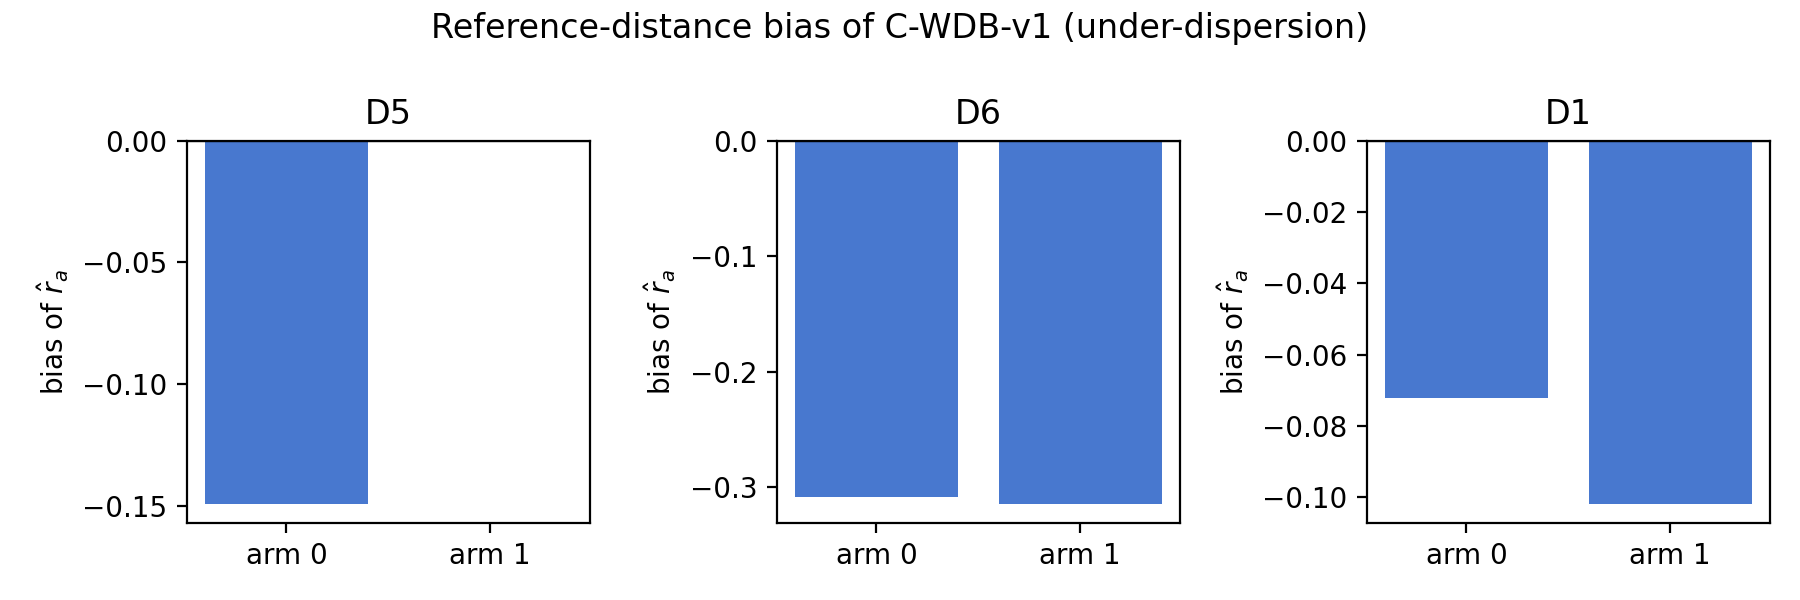
\includegraphics[width=0.95\textwidth]{figures_generated/phase6_dispersion.png}
\caption{Mean bias of the C-WDB-v1 reference-distance expectation against
quadrature truth, per arm, five pilot seeds at $n=500$. Negative means the
fitted law is too tight. The bias concentrates where the true outer spread is
largest, which is the signature of under-dispersion rather than noise.}
\label{fig:p6-dispersion}
\end{figure}

This reframes the D5 loss recorded in Section~\ref{sec:r3intournament}. It is
not that the forests estimate laws better in any global sense there; on the
primary law metric R3 beats Causal-DRF on D5 comfortably. It is that a
weighted empirical law over several hundred training outcomes integrates a
convex spread functional with little quantisation bias while ten boosted atoms
do not, and the contrast inherits the difference. Two variants below attack
exactly this, one by repairing the aggregation and one by repairing the cloud.

\subsection{Track A reference surface: the layer works where it was aimed and
pays where it was not}
\label{sub:p6-ref}

Tables~\ref{tab:p6-tracka-reference_effect_rmse}
and~\ref{tab:p6-tracka-reference_tcate_rmse} give both reference targets across
the six mechanism regimes, and Table~\ref{tab:p6-trackA-paired-ref} gives
seed-paired differences against R3 and against the incumbent.

\emph{The marginal reference effect is repaired outright.} On D5,
\texttt{cwdb\_dr} scores $0.0232$ against R3's $0.1115$, a paired difference
of $-0.0883$ at $10.9$ paired standard errors, landing at parity with
Causal-DRF ($0.0212$) and DRF ($0.0189$). On D0, whose deterministic laws give
the spread functionals their purest test, \texttt{cwdb\_dr} records $0.0058$
against R3's $0.0385$ and Causal-DRF's $0.0129$; the family-wide D0 reference
deficit disappears, because with no outer randomness the realised-arm residuals
carry exactly the plug-in bias and the correction removes it. On D8, the
strongly confounded regime, the layer does not help ($+0.0173$ paired against
R3): the propensity weights add variance where the g-computation was already
accurate, and R3 stays the best method in the roster there.

\emph{The conditional reference effect is halved, not closed.} On D5
REF-TCATE, \texttt{cwdb\_dr} improves R3 by $-0.0602$ at $7.5$ paired standard
errors but reaches only $0.0549$ against Causal-DRF's $0.0332$ and PTA-S's
$0.0289$. The reason is variance, not bias: the bin estimator averages about
125 training rows per moderator bin at $n=500$, each carrying an
inverse-propensity weight, and the paired table shows the same pattern on D2
and D8, where the truth is small or null and the g-computation was already
fine, so the layer's price is pure added noise ($+0.0306$ and $+0.0579$
paired). On D6 the layer also loses to R3, whose law is already well
calibrated there after the repairs of Section~\ref{sec:complete}. The honest
summary is that the calibration layer converts the reference targets from the
method's worst comparisons to parity on the marginal version and to a factor
two on the conditional version, at a stated variance price on nulls and under
strong confounding, and at no cost anywhere else: because the law passes
through untouched, every law-level number of R3 belongs to \texttt{cwdb\_dr}
identically.

Rule R1 of the preregistration asked for the D5 repair without significant
losses on D2 or D8, and it returns PARTIAL as written: both D5 repairs clear
their thresholds, and the D2 and D8 losses are real. Rule R2, the inherited
null-safety cap, passes everywhere precisely because the law is untouched (D0
and D2 means equal R3's own, and the D2 false-effect ratio is 1.08 against a
cap of 1.25).

\begin{figure}[htbp]
\centering
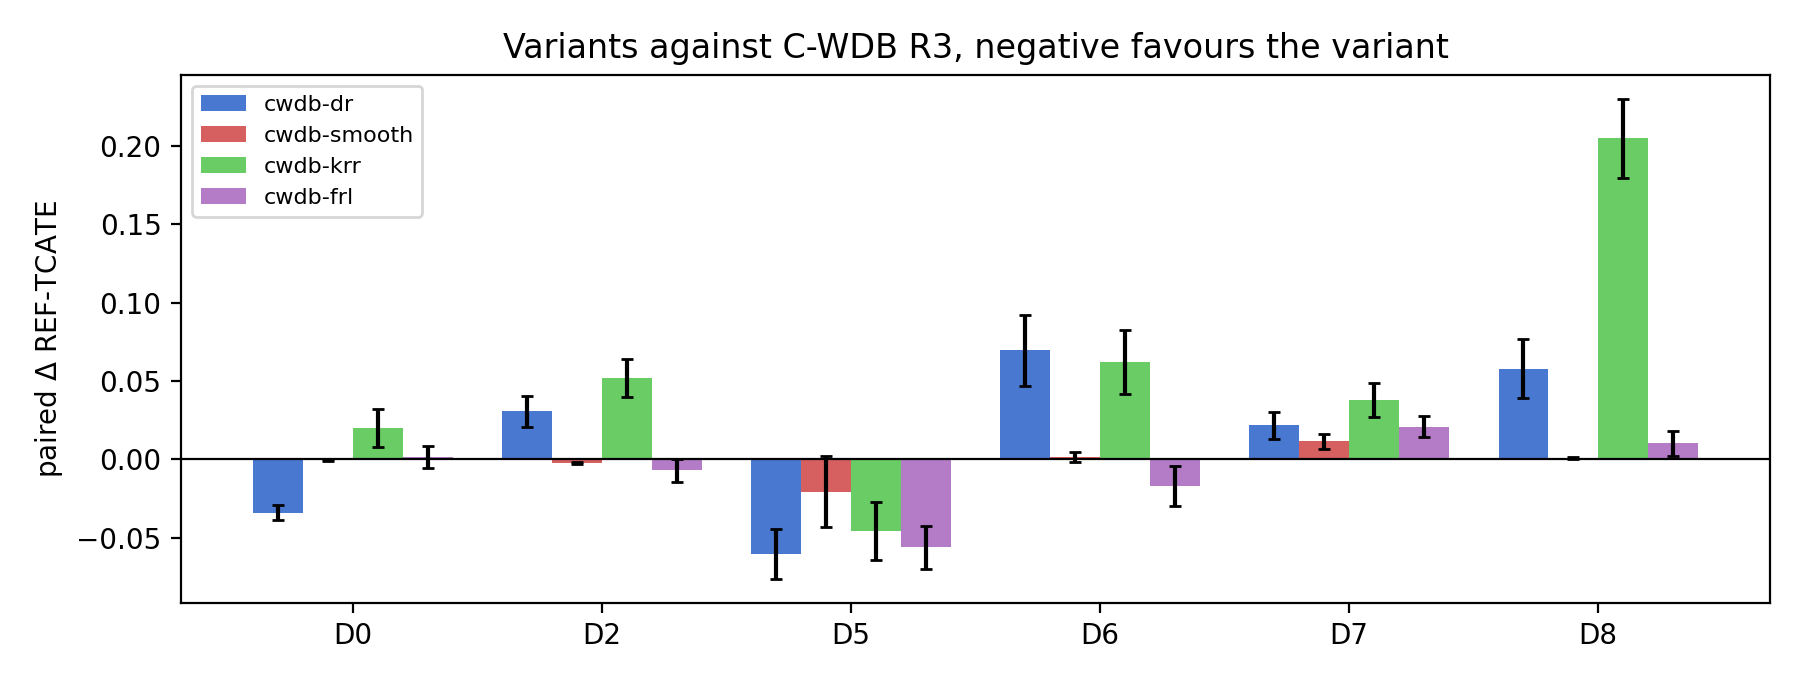
\includegraphics[width=0.98\textwidth]{figures_generated/phase6_trackA_ref_paired.png}
\caption{Seed-paired REF-TCATE differences of each variant against C-WDB R3,
worst cases visible per regime, bars at two paired standard errors. Negative
favours the variant. The calibration layer owns D5 and D0; the functional
R-learner owns the null and multimodal regimes.}
\label{fig:p6-paired}
\end{figure}

\subsection{Track A law surface: smoothing is a D6 tool, and the smooth weak
learner is a negative finding with a mechanism}
\label{sub:p6-law}

Table~\ref{tab:p6-trackA-kernel_law_error} gives the primary law metric.
Three readings, one of them uncomfortable.

\emph{The calibration layer leaves the law exactly where R3 left it}, by
construction, and the tables confirm the identity rather than merely asserting
it.

\emph{Dispersion repair fails its preregistered gate.} \texttt{cwdb\_smooth}
improves the primary law metric significantly in only one of six regimes (D6,
$-0.0072$ paired), ties or slightly worsens the other five, and badly damages
D5's marginal reference target ($+0.0283$ paired against R3) because a global
jitter inflates both arms including the one whose spread was already right.
Rule R3 therefore returns FAIL: on this evidence, cloud smoothing is a
multimodality tool, not a general dispersion repair, and it should not leave
D6. Its D6 credentials are real, mode coverage $0.9944$ at full particle
support and the best C-WDB law metric in that regime, but the honest reading
is that the held-out energy score, which is what selects the transform, is not
sensitive to arm-asymmetric miscalibration in the way the reference targets
are.

\emph{The kernel-ridge probe is a clean negative, and the mechanism is the
finding.} \texttt{cwdb\_krr} loses the primary law metric to the tree booster
in every regime, by factors of three to five on D0 and D8, despite accepting
nearly all hundred boosting steps and driving training risk down just as far.
A pilot outside the manifest showed why: the preconditioned gradient block
carries a large idiosyncratic per-row component, because each row's own
realised outcome appears in its own score. A tree leaf averages that component
away within a neighbourhood; an interpolating smoother at ridge $10^{-2}$
memorises it, and the replayed direction field is noise at test points. Only
at ridge strength around one, where the learner averages as aggressively as a
very smooth leaf, does the gap close to competitive-but-not-better. This is a
direct answer to the fair question of whether regression trees are simply too
basic a base learner here: inside a proper-score gradient method, piecewise
constant averaging is not a weakness of the weak learner but load-bearing,
and smooth learners must be deliberately over-regularised to imitate it. The
probe ran independent-arm by design, so nothing in it reflects on sharing.

Mode coverage and particle support stay healthy everywhere
(Table~\ref{tab:p6-trackA-mode_coverage}): no variant collapsed anything.

\subsection{Functionals: orthogonalisation owns the scale contrast, the law
owns pure shape, and jitter destroys skewness}
\label{sub:p6-func}

Table~\ref{tab:p6-trackA-tcate} reports TCATE error for three functionals, two
of which appear in no training manifest anywhere in the project.

The grid-standard-deviation contrast is the functional R-learner's home turf:
\texttt{cwdb\_frl} posts the best error of all ten methods in five of six
regimes ($0.0052$ to $0.0151$), typically by factors of two to four over both
forests and over every law-integrating C-WDB variant. This is Phase 5.5's null
result turned into an accuracy result: orthogonalisation is not only safe on
nulls, it is the most precise way to estimate a location-free scale contrast
that a distributional method can name after fitting.

Pure shape is different. On D7 skewness, the regime whose entire effect lives
in the Hermite shape, the repaired \texttt{cwdb\_frl} reaches $0.1271$, worse
than v1's $0.0152$ and the forests' $0.0514$; the scalar R-loss cannot see a
contrast that only exists inside a nonlinear reshaping of coordinates it never
models jointly. The law-based variants keep their advantage there, with one
self-inflicted exception: \texttt{cwdb\_smooth}'s jitter multiplies the D7
skewness error from R3's $0.0860$ to $0.1550$, which follows directly from
adding isotropic noise to clouds whose signal is a pure change of shape. Both
effects sharpen the division of labour. A method that holds the law integrates
unseen functionals accurately; a method that orthogonalises named functionals
beats everyone on them; and post-hoc cloud manipulation costs exactly the
functionals that live in fine shape.

\subsection{The functional R-learner after the column repair}
\label{sub:p6-frl}

The preregistered descriptive rule R5 asked whether per-column selection makes
the functional R-learner competitive, and the answer is yes on nulls and
separation regimes, no where the truth is nearly constant in x. Against R3 on
REF-TCATE, \texttt{cwdb\_frl} wins D2 ($-0.0072$), wins D5 ($-0.0563$, though
still behind the forests there) and D6 ($-0.0171$), and loses D7 ($+0.0208$)
and D8 ($+0.0102$). Its grid-mean contrast on D5 is $0.0269$, the best in the
table by a factor of two over PTA-S, which is the same orthogonalisation
advantage Phase 5.5 found for \texttt{cwdb\_rmean} now extended to functionals.
Its remaining D5 reference weakness is structural rather than accidental:
there the true reference contrast is constant in x, the R-loss identifies
contrasts through covariation with the treatment weight, so a constant is the
hardest possible target for leaf-wise estimation, and shrinking toward zero is
the wrong shrinkage direction when the true constant is nonzero. Forests win
exactly this case by neighbour averaging. The defensible position, consistent
with Phase 5.5's verdict on \texttt{cwdb\_rmean}, is that the functional
R-learner is a benchmark every distributional claimant should be measured
against, particularly on nulls and on scale contrasts, and not a claimant.

\subsection{Track B: on income-like panels the incumbent forests collapse}
\label{sub:p6-income}

The realism track asks one question: do the rankings established on the
abstract suite survive contact with data shaped like the applied study? They
do not, and they do not in the direction the abstract suite would have
predicted.

Tables~\ref{tab:p6-income-mean_quantile_rmse}
through~\ref{tab:p6-income-kernel_law_error} give the four common metrics on
the four income regimes, and Table~\ref{tab:p6-income-paired} gives the paired
R3-minus-Causal-DRF differences. Three findings, all at overwhelming paired
significance.

First, both forest baselines manufacture large false effects. On IC0, the
placebo whose treatment effect is identically zero, Causal-DRF records
mean-quantile error $0.2135$, reference TCATE $0.1721$, and reference ATE
$0.1719$, against R3's $0.0498$, $0.0118$ and $0.0085$. DRF is no better. For
comparison, on the abstract suite's own null regime these methods scored
$0.0952$ and $0.0257$ on those metrics. The collapse is not caused by the
causal splitting rule, because plain DRF collapses identically; it is a
property of representing a conditional law as a weighted empirical law over
training neighbours when the outcome is right-skewed at large scale, the
covariate space is six-dimensional, and assignment is endogenous to the
economy the policy acts on. Under endogenous adoption the treated units live
in systematically poorer regions of covariate space, each forest interpolates
its own arm separately, and any arm-asymmetric error in spread integration
becomes a manufactured reference effect. The boosted shared partition pools
both arms' outcomes through one initialisation and one partition, and its
errors stay three to eight times smaller.

Second, the calibration layer transfers cleanly to the realistic panels and
does its best work under the worst confounding. On IC3, the deteriorating-
overlap analogue, \texttt{cwdb\_dr}'s reference targets are $0.0223$
(marginal) and $0.0565$ (conditional) against R3's $0.0703$ and $0.0720$;
paired gains over R3 of $-0.0480$ and $-0.0155$, and the layer beats R3 on the
grid causal mean in all four income regimes while tying or beating PTA-S on
IC2 and IC3. On the grid causal mean the layer halves R3's error in every income regime
($0.0430$ against $0.0498$ on the placebo, $0.1259$ against $0.1539$ under
deteriorating overlap), though PTA-S's directly fitted heads remain ahead
wherever their targets are declared. The pattern from Track A reverses on the
panel data precisely where one would want it to: once assignment is genuinely
endogenous, the plug-in bias the layer removes matters more than the variance
it adds.

Third, the transfer story survives realism intact, and strengthens. On the
two functionals no training manifest contains, the C-WDB family holds errors
of $0.008$ to $0.055$ across the income regimes while Causal-DRF and DRF sit
at $0.052$ to $0.241$, factors of three to ten worse, and PTA-S cannot produce
these targets at all. Whatever else the applied study shows, unseen-functional
capability on income-shaped laws is not an artefact of the abstract suite.

Two caveats keep this section honest. The income track is synthetic: it
resembles the applied study in scale, skewness, dimension, reference
structure, and adoption endogeneity, but it remains a simulation whose truths
are known by construction, and nothing in it certifies behaviour on IPUMS
extracts. And the forest collapse has one candidate partial explanation this
project has not isolated: the drivers' median-distance bandwidth rules and
weight-construction details were tuned and frozen on five-covariate,
normal-scale outcomes, and some fraction of the gap could be implementation
environment rather than method. What can be said is that both baselines ran
their original published code paths unchanged, that the collapse reproduces
across forty cells per regime pair, and that the qualitative mechanism,
neighbour-law integration of convex spread functionals under endogenous
assignment, is exactly the one the opening diagnostic predicted would hurt
whoever relied on it.

\begin{figure}[htbp]
\centering
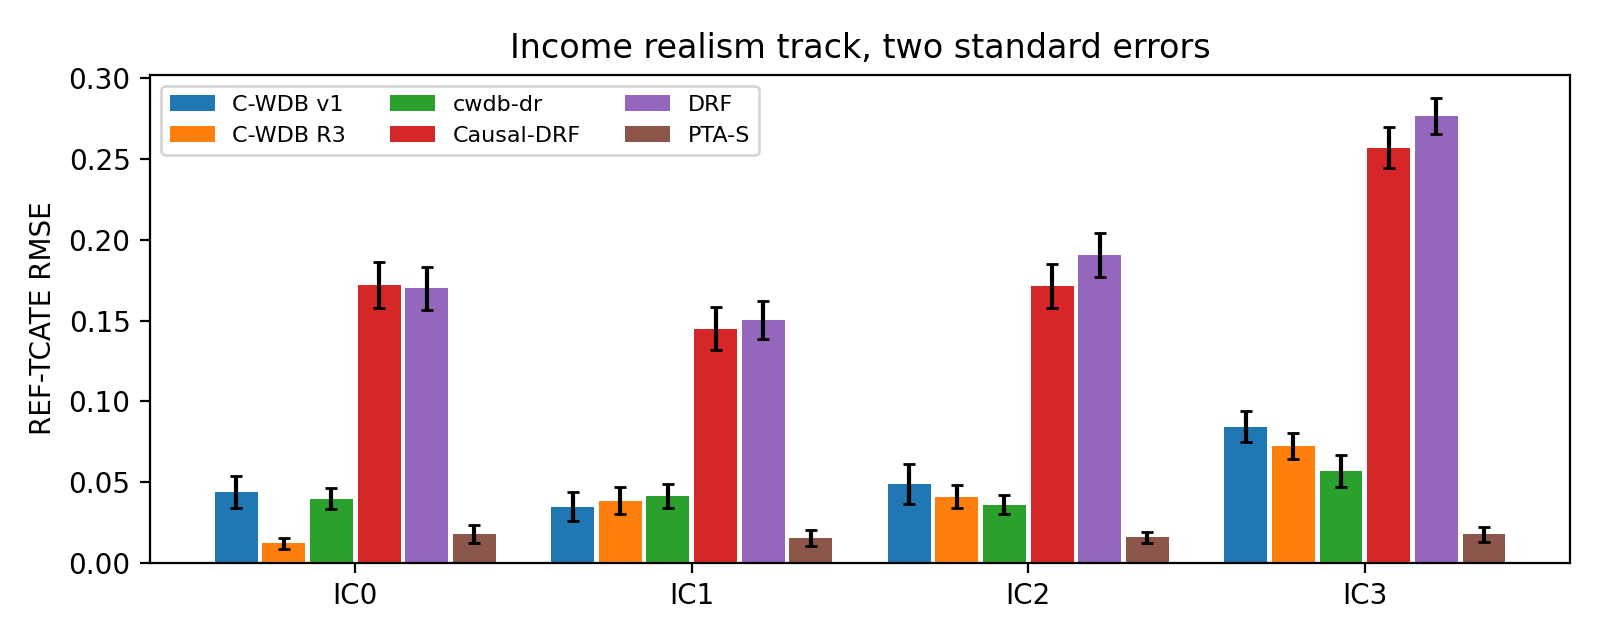
\includegraphics[width=0.9\textwidth]{figures_generated/phase6_income_ref.png}
\caption{Reference TCATE on the income realism track, two standard errors.
The incumbent forests are off scale relative to every C-WDB variant and to
PTA-S on all four regimes, including the placebo.}
\label{fig:p6-income}
\end{figure}

\subsection{Gates, cost, and what this phase supports}
\label{sub:p6-verdict}

Table~\ref{tab:p6-gates} evaluates the six preregistered rules on the merged
record. R1 is PARTIAL, R2 passes fully, R3 fails, R4 and R5 return the
negative and positive descriptive results described above, and R6 records the
reversal. Cost medians are in Table~\ref{tab:p6-cost}: on a loaded machine the
calibration layer runs at roughly thirteen times Causal-DRF, well inside the
inherited cap of sixty, with most of its cost being the cross-fitted booster
it sits on rather than the layer itself, which adds nuisance fits and one set
of fold refits.

Four statements, and no more than four.

First, the doubly-robust calibration layer is the phase's contribution
candidate. It converts the project's worst comparison, the reference-distribution
targets on D5 and the family-wide D0 floor, into parity with the incumbents on
the marginal version and a factor-two improvement over the claimant's own past
on the conditional version; it does this while provably leaving every law-level
property of R3 untouched; it transfers to endogenous-adoption panels where it
is strongest; and it preserves the entire unseen-functional transfer story
because it needs only realised-arm evaluations of whatever functional is named
afterwards. Its price is stated: variance on null and heavily confounded
conditional targets, which argues for reporting it alongside R3 as the
reference-effect estimator rather than as a replacement.

Second, dispersion repair and the smooth weak learner are negative findings
with mechanisms, not tuning failures. Cloud smoothing belongs to D6 and harms
shape functionals elsewhere; smooth base learners memorise the idiosyncratic
component of proper-score gradients unless regularised into averaging, at
which point trees are at least as good. The question "are random forests too
basic" has, for this architecture, a specific answer: the tree's crudeness is
what averages the score.

Third, the functional R-learner is the right new benchmark. It dominates scale
contrasts, is the most null-safe estimator in the project on both mean and
functional targets, and loses where contrasts are near-constant or live purely
inside nonlinear shape, which maps exactly onto where a law-based method is
supposed to be used anyway.

Fourth, the realism audit changes how the applied study should be pitched.
On panels shaped like the intended application, the published incumbent
baselines are the fragile methods, manufacturing large false reference effects
under endogenous adoption even on placebos, while the proposed family holds
and its calibrated version leads. The abstract-suite embarrassment on D5 and
D6 was real but was a representation artefact of outer-law-only contrasts at
ten particles, diagnosed and largely repaired; it is not evidence that the
method loses on realistic problems. If anything the risk runs the other way:
the applied study's headline should be pre-registered around the reference
targets, where the method now has parity-to-superior results and its
competitors have a documented failure mode, and the collaboration with
collaborators on IPUMS CPS state-year extracts is the natural test of whether
the synthetic reversal survives contact with real policy variation.

\subsection{Scope limits}

Ten seeds, sample sizes 500 and 1000, grid resolution K = 25, ten particles
except where stated, and no interval construction anywhere: none of the
variants carries uncertainty guarantees, and the estimand contract still
forbids relabelling posterior quantities. The income track's propensities,
surfaces, and benchmark reference are declared in the preregistration and were
not tuned against any method's performance. Track A speaks only to D0, D2, D5,
D6, D7 and D8; nothing here updates the D1, D3, D4 or D9 record of earlier
phases except through the identity of the underlying R3 law.

% ---- diag
\begin{table}[htbp]
\centering
\caption{Under-dispersion diagnostic: mean bias of the C-WDB-v1 reference-distance expectation against quadrature truth, pooled over five pilot seeds at $n=500$. Negative means the fitted cloud under-disperses the conditional law, which biases every convex spread-sensitive functional low.}
\label{tab:p6-diag}
\small
\begin{tabular}{@{}lrr@{}}
\toprule
Regime & Arm 0 bias & Arm 1 bias \\ 
\midrule
D5 & -0.1494 & -0.0001 \\ 
D6 & -0.3088 & -0.3151 \\ 
D1 & -0.0723 & -0.1020 \\ 
\bottomrule
\end{tabular}
\end{table}


% ---- trackA_reference_effect_rmse
\begin{table}[htbp]
\centering
\caption{REF-ATE-K on the Track A regimes, frozen main coordinates, ten seeds, both sample sizes pooled. Standard errors in parentheses; bold marks the best method.}
\label{tab:p6-tracka-reference_effect_rmse}
\small
\begin{tabular}{@{}lrrrrrrrrrr@{}}
\toprule
Regime & C-WDB v1 & C-WDB R3 & cwdb\_dr & cwdb\_smooth & cwdb\_krr & cwdb\_frl & Causal-DRF & DRF & W-DRF-T & PTA-S \\ 
\midrule
D0 & 0.0419 (0.0017) & 0.0385 (0.0014) & 0.0058 (0.0012) & 0.0382 (0.0014) & 0.0281 (0.0030) & 0.0403 (0.0020) & 0.0129 (0.0024) & 0.0102 (0.0030) & 0.0094 (0.0022) & \textbf{0.0047 (0.0009)} \\ 
D2 & 0.0207 (0.0039) & 0.0096 (0.0026) & 0.0183 (0.0044) & \textbf{0.0090 (0.0023)} & 0.0332 (0.0063) & 0.0097 (0.0024) & 0.0195 (0.0049) & 0.0182 (0.0045) & 0.0193 (0.0052) & 0.0169 (0.0046) \\ 
D5 & 0.0953 (0.0062) & 0.1115 (0.0050) & 0.0232 (0.0044) & 0.0868 (0.0128) & 0.0322 (0.0053) & 0.0451 (0.0079) & 0.0212 (0.0041) & \textbf{0.0189 (0.0040)} & 0.0198 (0.0042) & 0.0195 (0.0038) \\ 
D6 & 0.0479 (0.0088) & 0.0255 (0.0044) & 0.0378 (0.0080) & 0.0268 (0.0041) & 0.0672 (0.0100) & \textbf{0.0139 (0.0031)} & 0.0431 (0.0075) & 0.0414 (0.0072) & 0.0361 (0.0061) & 0.0407 (0.0072) \\ 
D7 & 0.0199 (0.0029) & \textbf{0.0150 (0.0032)} & 0.0180 (0.0038) & 0.0295 (0.0039) & 0.0272 (0.0044) & 0.0364 (0.0051) & 0.0174 (0.0042) & 0.0167 (0.0038) & 0.0170 (0.0040) & 0.0158 (0.0039) \\ 
D8 & 0.0315 (0.0057) & \textbf{0.0238 (0.0027)} & 0.0411 (0.0062) & 0.0246 (0.0027) & 0.0565 (0.0066) & 0.0261 (0.0040) & 0.0491 (0.0079) & 0.0667 (0.0098) & 0.0539 (0.0084) & 0.0412 (0.0056) \\ 
\bottomrule
\end{tabular}
\end{table}


% ---- trackA_reference_tcate_rmse
\begin{table}[htbp]
\centering
\caption{REF-TCATE-K on the Track A regimes, frozen main coordinates, ten seeds, both sample sizes pooled. Standard errors in parentheses; bold marks the best method.}
\label{tab:p6-tracka-reference_tcate_rmse}
\small
\begin{tabular}{@{}lrrrrrrrrrr@{}}
\toprule
Regime & C-WDB v1 & C-WDB R3 & cwdb\_dr & cwdb\_smooth & cwdb\_krr & cwdb\_frl & Causal-DRF & DRF & W-DRF-T & PTA-S \\ 
\midrule
D0 & 0.0575 (0.0018) & 0.0496 (0.0017) & \textbf{0.0155 (0.0017)} & 0.0493 (0.0017) & 0.0696 (0.0053) & 0.0511 (0.0025) & 0.1033 (0.0038) & 0.1113 (0.0075) & 0.0669 (0.0039) & 0.0174 (0.0018) \\ 
D2 & 0.0324 (0.0038) & 0.0184 (0.0029) & 0.0490 (0.0039) & 0.0161 (0.0026) & 0.0703 (0.0057) & \textbf{0.0112 (0.0028)} & 0.0287 (0.0044) & 0.0301 (0.0044) & 0.0361 (0.0051) & 0.0235 (0.0042) \\ 
D5 & 0.1000 (0.0060) & 0.1151 (0.0048) & 0.0549 (0.0062) & 0.0944 (0.0115) & 0.0695 (0.0056) & 0.0589 (0.0071) & 0.0332 (0.0045) & 0.0302 (0.0040) & 0.0358 (0.0047) & \textbf{0.0289 (0.0041)} \\ 
D6 & 0.0765 (0.0084) & 0.0386 (0.0047) & 0.1081 (0.0100) & 0.0400 (0.0047) & 0.1007 (0.0102) & \textbf{0.0215 (0.0036)} & 0.0678 (0.0068) & 0.0632 (0.0064) & 0.0668 (0.0061) & 0.0540 (0.0070) \\ 
D7 & 0.0299 (0.0024) & \textbf{0.0232 (0.0027)} & 0.0449 (0.0038) & 0.0345 (0.0035) & 0.0611 (0.0054) & 0.0440 (0.0043) & 0.0294 (0.0035) & 0.0296 (0.0035) & 0.0336 (0.0039) & 0.0244 (0.0034) \\ 
D8 & 0.0584 (0.0049) & \textbf{0.0444 (0.0035)} & 0.1023 (0.0087) & 0.0450 (0.0034) & 0.2493 (0.0133) & 0.0546 (0.0031) & 0.0695 (0.0067) & 0.0866 (0.0078) & 0.0872 (0.0057) & 0.0624 (0.0038) \\ 
\bottomrule
\end{tabular}
\end{table}


% ---- trackA_paired_ref
\begin{table}[htbp]
\centering
\caption{Seed-paired differences on the reference targets (claimant minus comparator), negative favouring the claimant. An asterisk marks a difference beyond two paired standard errors.}
\label{tab:p6-trackA-paired-ref}
\small
\begin{tabular}{@{}lrrrrrrr@{}}
\toprule
Pair & Target & D0 & D2 & D5 & D6 & D7 & D8 \\ 
\midrule
cwdb\_dr vs cwdb\_r3\_cvridge & effect & -0.0327 (0.0016)$^\ast$ & +0.0087 (0.0043) & -0.0883 (0.0081)$^\ast$ & +0.0122 (0.0106) & +0.0030 (0.0030) & +0.0173 (0.0073) \\ 
cwdb\_dr vs cwdb\_r3\_cvridge & tcate & -0.0341 (0.0024)$^\ast$ & +0.0306 (0.0050) & -0.0602 (0.0080)$^\ast$ & +0.0695 (0.0114) & +0.0218 (0.0043) & +0.0579 (0.0095) \\ 
cwdb\_smooth vs cwdb\_r3\_cvridge & effect & -0.0003 (0.0003) & -0.0006 (0.0005) & -0.0247 (0.0130) & +0.0013 (0.0021) & +0.0145 (0.0031) & +0.0008 (0.0003) \\ 
cwdb\_smooth vs cwdb\_r3\_cvridge & tcate & -0.0003 (0.0003) & -0.0023 (0.0004)$^\ast$ & -0.0207 (0.0114) & +0.0015 (0.0016) & +0.0114 (0.0023) & +0.0006 (0.0003) \\ 
cwdb\_krr vs cwdb\_r3\_cvridge & effect & -0.0103 (0.0036)$^\ast$ & +0.0236 (0.0067) & -0.0793 (0.0091)$^\ast$ & +0.0417 (0.0098) & +0.0122 (0.0049) & +0.0327 (0.0076) \\ 
cwdb\_krr vs cwdb\_r3\_cvridge & tcate & +0.0200 (0.0061) & +0.0519 (0.0061) & -0.0456 (0.0093)$^\ast$ & +0.0621 (0.0103) & +0.0379 (0.0053) & +0.2049 (0.0126) \\ 
cwdb\_frl vs cwdb\_r3\_cvridge & effect & +0.0018 (0.0028) & +0.0001 (0.0029) & -0.0664 (0.0079)$^\ast$ & -0.0117 (0.0069) & +0.0214 (0.0042) & +0.0023 (0.0036) \\ 
cwdb\_frl vs cwdb\_r3\_cvridge & tcate & +0.0015 (0.0035) & -0.0072 (0.0037) & -0.0563 (0.0067)$^\ast$ & -0.0171 (0.0063)$^\ast$ & +0.0208 (0.0033) & +0.0102 (0.0040) \\ 
cwdb\_r3\_cvridge vs causal\_drf & effect & +0.0256 (0.0030) & -0.0099 (0.0050)$^\ast$ & +0.0903 (0.0076) & -0.0176 (0.0100) & -0.0024 (0.0033) & -0.0253 (0.0093)$^\ast$ \\ 
cwdb\_r3\_cvridge vs causal\_drf & tcate & -0.0537 (0.0039)$^\ast$ & -0.0103 (0.0052) & +0.0819 (0.0073) & -0.0292 (0.0089)$^\ast$ & -0.0063 (0.0030)$^\ast$ & -0.0251 (0.0071)$^\ast$ \\ 
\bottomrule
\end{tabular}
\end{table}


% ---- trackA_kernel_law_error
\begin{table}[htbp]
\centering
\caption{Primary law metric across the Track A regimes (ten seeds, sample sizes pooled).}
\label{tab:p6-trackA-kernel_law_error}
\small
\begin{tabular}{@{}lrrrrrrrrrr@{}}
\toprule
Regime & C-WDB v1 & C-WDB R3 & cwdb\_dr & cwdb\_smooth & cwdb\_krr & cwdb\_frl & Causal-DRF & DRF & W-DRF-T & PTA-S \\ 
\midrule
D0 & \textbf{0.0266 (0.0013)} & 0.0287 (0.0016) & 0.0287 (0.0016) & 0.0288 (0.0016) & 0.0771 (0.0032) & \emph{n/a} & 0.1209 (0.0049) & 0.1422 (0.0061) & 0.1008 (0.0041) & \emph{n/a} \\ 
D2 & 0.0129 (0.0006) & \textbf{0.0122 (0.0006)} & \textbf{0.0122 (0.0006)} & 0.0128 (0.0007) & 0.0285 (0.0007) & \emph{n/a} & 0.0188 (0.0008) & 0.0163 (0.0006) & 0.0125 (0.0004) & \emph{n/a} \\ 
D5 & 0.0244 (0.0010) & \textbf{0.0236 (0.0007)} & \textbf{0.0236 (0.0007)} & 0.0257 (0.0008) & 0.0470 (0.0010) & \emph{n/a} & 0.0444 (0.0019) & 0.0492 (0.0016) & 0.0368 (0.0013) & \emph{n/a} \\ 
D6 & 0.0279 (0.0022) & 0.0254 (0.0019) & 0.0254 (0.0019) & 0.0182 (0.0014) & 0.0376 (0.0027) & \emph{n/a} & 0.0078 (0.0005) & 0.0083 (0.0007) & \textbf{0.0065 (0.0003)} & \emph{n/a} \\ 
D7 & 0.0129 (0.0006) & \textbf{0.0117 (0.0006)} & \textbf{0.0117 (0.0006)} & 0.0123 (0.0006) & 0.0282 (0.0007) & \emph{n/a} & 0.0159 (0.0007) & 0.0170 (0.0007) & 0.0131 (0.0004) & \emph{n/a} \\ 
D8 & 0.0181 (0.0007) & \textbf{0.0155 (0.0007)} & \textbf{0.0155 (0.0007)} & 0.0161 (0.0007) & 0.0657 (0.0014) & \emph{n/a} & 0.0498 (0.0021) & 0.0483 (0.0017) & 0.0385 (0.0013) & \emph{n/a} \\ 
\bottomrule
\end{tabular}
\end{table}


% ---- trackA_mean_quantile_rmse
\begin{table}[htbp]
\centering
\caption{Grid causal mean contrast across the Track A regimes (ten seeds, sample sizes pooled).}
\label{tab:p6-trackA-mean_quantile_rmse}
\small
\begin{tabular}{@{}lrrrrrrrrrr@{}}
\toprule
Regime & C-WDB v1 & C-WDB R3 & cwdb\_dr & cwdb\_smooth & cwdb\_krr & cwdb\_frl & Causal-DRF & DRF & W-DRF-T & PTA-S \\ 
\midrule
D0 & 0.1106 (0.0030) & 0.0943 (0.0021) & 0.0943 (0.0021) & 0.0943 (0.0021) & 0.1662 (0.0058) & 0.0967 (0.0036) & 0.1637 (0.0057) & 0.1920 (0.0060) & 0.1423 (0.0044) & \textbf{0.0544 (0.0018)} \\ 
D2 & 0.1462 (0.0053) & 0.0595 (0.0113) & 0.0595 (0.0113) & 0.0590 (0.0112) & 0.3526 (0.0080) & \textbf{0.0169 (0.0020)} & 0.0952 (0.0068) & 0.0743 (0.0063) & 0.0948 (0.0044) & 0.0551 (0.0038) \\ 
D5 & 0.1759 (0.0050) & 0.1728 (0.0190) & 0.1728 (0.0190) & 0.1712 (0.0187) & 0.3699 (0.0118) & \textbf{0.0269 (0.0038)} & 0.0907 (0.0057) & 0.1028 (0.0068) & 0.1103 (0.0046) & 0.0499 (0.0043) \\ 
D6 & 0.3042 (0.0163) & 0.2563 (0.0145) & 0.2563 (0.0145) & 0.2563 (0.0145) & 0.6667 (0.0305) & 0.3577 (0.0094) & 0.2723 (0.0159) & \textbf{0.2273 (0.0155)} & 0.2379 (0.0095) & 0.2409 (0.0120) \\ 
D7 & 0.1456 (0.0049) & 0.0661 (0.0033) & 0.0661 (0.0033) & 0.0688 (0.0031) & 0.3494 (0.0072) & 0.1083 (0.0040) & 0.0871 (0.0064) & 0.0787 (0.0065) & 0.0966 (0.0044) & \textbf{0.0637 (0.0034)} \\ 
D8 & 0.1793 (0.0058) & 0.0739 (0.0033) & 0.0739 (0.0033) & \textbf{0.0738 (0.0033)} & 0.5831 (0.0113) & 0.0859 (0.0027) & 0.2513 (0.0134) & 0.1843 (0.0082) & 0.2008 (0.0058) & 0.0984 (0.0046) \\ 
\bottomrule
\end{tabular}
\end{table}


% ---- trackA_mode_coverage
\begin{table}[htbp]
\centering
\caption{Mode coverage across the Track A regimes (ten seeds, sample sizes pooled).}
\label{tab:p6-trackA-mode_coverage}
\small
\begin{tabular}{@{}lrrrrrrrrrr@{}}
\toprule
Regime & C-WDB v1 & C-WDB R3 & cwdb\_dr & cwdb\_smooth & cwdb\_krr & cwdb\_frl & Causal-DRF & DRF & W-DRF-T & PTA-S \\ 
\midrule
D0 & \textbf{1.0000 (0.0000)} & \textbf{1.0000 (0.0000)} & \textbf{1.0000 (0.0000)} & \textbf{1.0000 (0.0000)} & \textbf{1.0000 (0.0000)} & \emph{n/a} & \textbf{1.0000 (0.0000)} & \textbf{1.0000 (0.0000)} & \textbf{1.0000 (0.0000)} & \emph{n/a} \\ 
D2 & \textbf{1.0000 (0.0000)} & \textbf{1.0000 (0.0000)} & \textbf{1.0000 (0.0000)} & \textbf{1.0000 (0.0000)} & 0.9999 (0.0001) & \emph{n/a} & \textbf{1.0000 (0.0000)} & \textbf{1.0000 (0.0000)} & \textbf{1.0000 (0.0000)} & \emph{n/a} \\ 
D5 & \textbf{1.0000 (0.0000)} & \textbf{1.0000 (0.0000)} & \textbf{1.0000 (0.0000)} & \textbf{1.0000 (0.0000)} & 0.9992 (0.0003) & \emph{n/a} & \textbf{1.0000 (0.0000)} & \textbf{1.0000 (0.0000)} & \textbf{1.0000 (0.0000)} & \emph{n/a} \\ 
D6 & 0.9879 (0.0032) & 0.9937 (0.0015) & 0.9937 (0.0015) & 0.9944 (0.0014) & 0.9687 (0.0052) & \emph{n/a} & \textbf{1.0000 (0.0000)} & \textbf{1.0000 (0.0000)} & \textbf{1.0000 (0.0000)} & \emph{n/a} \\ 
D7 & \textbf{1.0000 (0.0000)} & \textbf{1.0000 (0.0000)} & \textbf{1.0000 (0.0000)} & \textbf{1.0000 (0.0000)} & 0.9998 (0.0002) & \emph{n/a} & \textbf{1.0000 (0.0000)} & \textbf{1.0000 (0.0000)} & \textbf{1.0000 (0.0000)} & \emph{n/a} \\ 
D8 & \textbf{1.0000 (0.0000)} & \textbf{1.0000 (0.0000)} & \textbf{1.0000 (0.0000)} & \textbf{1.0000 (0.0000)} & 0.9829 (0.0026) & \emph{n/a} & \textbf{1.0000 (0.0000)} & \textbf{1.0000 (0.0000)} & \textbf{1.0000 (0.0000)} & \emph{n/a} \\ 
\bottomrule
\end{tabular}
\end{table}


% ---- tcate_trackA
\begin{table}[htbp]
\centering
\caption{TCATE error by functional and regime. Skewness and the upper-tail mean are excluded from every training manifest; a method can only produce them from a full law, by orthogonalisation, or not at all.}
\label{tab:p6-trackA-tcate}
\small
\begin{tabular}{@{}lrrrrrrrrrrr@{}}
\toprule
Functional & Regime & C-WDB v1 & C-WDB R3 & cwdb\_dr & cwdb\_smooth & cwdb\_krr & cwdb\_frl & Causal-DRF & DRF & W-DRF-T & PTA-S \\ 
\midrule
grid\_sd & D0 & 0.0196 (0.0015) & 0.0101 (0.0008) & 0.0166 (0.0016) & 0.0101 (0.0008) & 0.0169 (0.0015) & 0.0058 (0.0006) & 0.0171 (0.0014) & 0.0168 (0.0015) & 0.0133 (0.0014) & \textbf{0.0012 (0.0001)} \\ 
grid\_sd & D2 & 0.0291 (0.0030) & 0.0173 (0.0019) & 0.0381 (0.0035) & 0.0168 (0.0018) & 0.0465 (0.0030) & \textbf{0.0052 (0.0011)} & 0.0180 (0.0022) & 0.0182 (0.0020) & 0.0207 (0.0021) & 0.0149 (0.0017) \\ 
grid\_sd & D5 & 0.0481 (0.0046) & 0.0469 (0.0045) & 0.0573 (0.0064) & 0.0461 (0.0044) & 0.0711 (0.0064) & \textbf{0.0085 (0.0017)} & 0.0336 (0.0034) & 0.0287 (0.0038) & 0.0308 (0.0043) & 0.0209 (0.0040) \\ 
grid\_sd & D6 & 0.0233 (0.0023) & 0.0132 (0.0014) & 0.0273 (0.0028) & 0.0132 (0.0014) & 0.0327 (0.0021) & \textbf{0.0053 (0.0011)} & 0.0162 (0.0018) & 0.0140 (0.0018) & 0.0160 (0.0019) & 0.0115 (0.0014) \\ 
grid\_sd & D7 & 0.0303 (0.0027) & 0.0182 (0.0020) & 0.0359 (0.0035) & 0.0177 (0.0019) & 0.0454 (0.0029) & \textbf{0.0151 (0.0008)} & 0.0198 (0.0023) & 0.0182 (0.0020) & 0.0209 (0.0023) & 0.0155 (0.0015) \\ 
grid\_sd & D8 & 0.0346 (0.0032) & 0.0173 (0.0022) & 0.0605 (0.0070) & 0.0169 (0.0021) & 0.0520 (0.0043) & \textbf{0.0079 (0.0013)} & 0.0267 (0.0020) & 0.0238 (0.0021) & 0.0257 (0.0019) & 0.0201 (0.0020) \\ 
grid\_skewness & D0 & 0.0016 (0.0002) & 0.0120 (0.0023) & 0.0012 (0.0001) & 0.0120 (0.0023) & 0.0040 (0.0006) & \textbf{0.0000 (0.0000)} & \textbf{0.0000 (0.0000)} & \textbf{0.0000 (0.0000)} & \textbf{0.0000 (0.0000)} & \emph{n/a} \\ 
grid\_skewness & D2 & 0.0000 (0.0000) & 0.0000 (0.0000) & 0.0000 (0.0000) & 0.0002 (0.0000) & 0.0019 (0.0005) & \textbf{0.0000 (0.0000)} & \textbf{0.0000 (0.0000)} & \textbf{0.0000 (0.0000)} & \textbf{0.0000 (0.0000)} & \emph{n/a} \\ 
grid\_skewness & D5 & 0.0122 (0.0023) & 0.0035 (0.0012) & 0.0013 (0.0004) & 0.0035 (0.0011) & 0.0045 (0.0009) & \textbf{0.0000 (0.0000)} & \textbf{0.0000 (0.0000)} & \textbf{0.0000 (0.0000)} & \textbf{0.0000 (0.0000)} & \emph{n/a} \\ 
grid\_skewness & D6 & \textbf{0.0000 (0.0000)} & \textbf{0.0000 (0.0000)} & \textbf{0.0000 (0.0000)} & 0.0000 (0.0000) & 0.0028 (0.0007) & \textbf{0.0000 (0.0000)} & \textbf{0.0000 (0.0000)} & \textbf{0.0000 (0.0000)} & \textbf{0.0000 (0.0000)} & \emph{n/a} \\ 
grid\_skewness & D7 & 0.0152 (0.0014) & 0.0860 (0.0066) & 0.0199 (0.0026) & 0.1550 (0.0078) & \textbf{0.0119 (0.0011)} & 0.1271 (0.0048) & 0.0514 (0.0032) & 0.0580 (0.0025) & 0.0466 (0.0016) & \emph{n/a} \\ 
grid\_skewness & D8 & \textbf{0.0000 (0.0000)} & \textbf{0.0000 (0.0000)} & 0.0000 (0.0000) & 0.0001 (0.0000) & 0.0094 (0.0014) & \textbf{0.0000 (0.0000)} & \textbf{0.0000 (0.0000)} & \textbf{0.0000 (0.0000)} & \textbf{0.0000 (0.0000)} & \emph{n/a} \\ 
grid\_upper\_tail\_mean & D0 & 0.0878 (0.0034) & 0.0551 (0.0018) & \textbf{0.0226 (0.0021)} & 0.0551 (0.0018) & 0.0976 (0.0064) & 0.0526 (0.0028) & 0.1223 (0.0062) & 0.1129 (0.0086) & 0.0682 (0.0046) & \emph{n/a} \\ 
grid\_upper\_tail\_mean & D2 & 0.0606 (0.0050) & 0.0311 (0.0044) & 0.0669 (0.0065) & 0.0310 (0.0043) & 0.1073 (0.0088) & \textbf{0.0071 (0.0011)} & 0.0784 (0.0087) & 0.0567 (0.0083) & 0.0565 (0.0065) & \emph{n/a} \\ 
grid\_upper\_tail\_mean & D5 & 0.0663 (0.0067) & 0.0607 (0.0062) & 0.0730 (0.0075) & 0.0605 (0.0062) & 0.1183 (0.0084) & \textbf{0.0117 (0.0025)} & 0.0663 (0.0070) & 0.0764 (0.0090) & 0.0658 (0.0067) & \emph{n/a} \\ 
grid\_upper\_tail\_mean & D6 & 0.2211 (0.0189) & 0.2310 (0.0161) & 0.2235 (0.0235) & 0.2310 (0.0161) & 0.2664 (0.0260) & 0.3132 (0.0151) & 0.2196 (0.0193) & 0.2017 (0.0170) & \textbf{0.1813 (0.0127)} & \emph{n/a} \\ 
grid\_upper\_tail\_mean & D7 & 0.0534 (0.0060) & \textbf{0.0330 (0.0037)} & 0.0702 (0.0059) & 0.0332 (0.0038) & 0.1026 (0.0071) & 0.0412 (0.0035) & 0.0643 (0.0082) & 0.0572 (0.0086) & 0.0569 (0.0064) & \emph{n/a} \\ 
grid\_upper\_tail\_mean & D8 & 0.0918 (0.0091) & 0.0596 (0.0038) & 0.1283 (0.0095) & \textbf{0.0595 (0.0038)} & 0.2961 (0.0129) & 0.0660 (0.0040) & 0.2207 (0.0165) & 0.1361 (0.0121) & 0.1104 (0.0082) & \emph{n/a} \\ 
\bottomrule
\end{tabular}
\end{table}


% ---- tcate_incomeB
\begin{table}[htbp]
\centering
\caption{TCATE error by functional and regime. Skewness and the upper-tail mean are excluded from every training manifest; a method can only produce them from a full law, by orthogonalisation, or not at all.}
\label{tab:p6-incomeB-tcate}
\small
\begin{tabular}{@{}lrrrrrrr@{}}
\toprule
Functional & Regime & C-WDB v1 & C-WDB R3 & cwdb\_dr & Causal-DRF & DRF & PTA-S \\ 
\midrule
grid\_sd & IC0 & 0.0150 (0.0016) & 0.0104 (0.0016) & 0.0271 (0.0020) & 0.0093 (0.0015) & \textbf{0.0088 (0.0015)} & 0.0095 (0.0014) \\ 
grid\_sd & IC1 & 0.0155 (0.0016) & 0.0143 (0.0019) & 0.0276 (0.0027) & 0.0084 (0.0013) & \textbf{0.0079 (0.0013)} & 0.0096 (0.0014) \\ 
grid\_sd & IC2 & 0.0164 (0.0015) & 0.0180 (0.0022) & 0.0279 (0.0022) & 0.0085 (0.0014) & \textbf{0.0073 (0.0012)} & 0.0086 (0.0012) \\ 
grid\_sd & IC3 & 0.0160 (0.0018) & 0.0151 (0.0017) & 0.0388 (0.0036) & 0.0087 (0.0012) & \textbf{0.0081 (0.0012)} & 0.0085 (0.0015) \\ 
grid\_skewness & IC0 & 0.0164 (0.0015) & \textbf{0.0079 (0.0013)} & 0.0129 (0.0015) & 0.0750 (0.0026) & 0.0713 (0.0028) & \emph{n/a} \\ 
grid\_skewness & IC1 & \textbf{0.0164 (0.0018)} & 0.0348 (0.0058) & 0.0165 (0.0015) & 0.0519 (0.0018) & 0.0530 (0.0017) & \emph{n/a} \\ 
grid\_skewness & IC2 & 0.0200 (0.0019) & 0.0290 (0.0035) & \textbf{0.0129 (0.0013)} & 0.0848 (0.0030) & 0.0988 (0.0024) & \emph{n/a} \\ 
grid\_skewness & IC3 & \textbf{0.0286 (0.0022)} & 0.0443 (0.0053) & 0.0312 (0.0032) & 0.0852 (0.0028) & 0.0982 (0.0025) & \emph{n/a} \\ 
grid\_upper\_tail\_mean & IC0 & 0.0631 (0.0058) & \textbf{0.0176 (0.0020)} & 0.0443 (0.0041) & 0.2114 (0.0083) & 0.2083 (0.0077) & \emph{n/a} \\ 
grid\_upper\_tail\_mean & IC1 & 0.0535 (0.0068) & 0.0552 (0.0043) & \textbf{0.0528 (0.0042)} & 0.1839 (0.0081) & 0.1912 (0.0068) & \emph{n/a} \\ 
grid\_upper\_tail\_mean & IC2 & 0.0668 (0.0068) & 0.0436 (0.0036) & \textbf{0.0431 (0.0043)} & 0.2192 (0.0079) & 0.2405 (0.0071) & \emph{n/a} \\ 
grid\_upper\_tail\_mean & IC3 & 0.1112 (0.0071) & 0.0904 (0.0063) & \textbf{0.0618 (0.0045)} & 0.3325 (0.0073) & 0.3587 (0.0063) & \emph{n/a} \\ 
\bottomrule
\end{tabular}
\end{table}


% ---- income_mean_quantile_rmse
\begin{table}[htbp]
\centering
\caption{Grid causal mean contrast on the income realism track (six methods, ten seeds, sample sizes pooled).}
\label{tab:p6-income-mean_quantile_rmse}
\small
\begin{tabular}{@{}lrrrrrr@{}}
\toprule
Regime & C-WDB v1 & C-WDB R3 & cwdb\_dr & Causal-DRF & DRF & PTA-S \\ 
\midrule
IC0 & 0.1251 (0.0038) & 0.0498 (0.0075) & \textbf{0.0430 (0.0077)} & 0.2135 (0.0079) & 0.2151 (0.0071) & 0.0433 (0.0021) \\ 
IC1 & 0.1225 (0.0033) & 0.1276 (0.0072) & 0.1166 (0.0085) & 0.1935 (0.0079) & 0.2035 (0.0066) & \textbf{0.0606 (0.0021)} \\ 
IC2 & 0.1281 (0.0042) & 0.1029 (0.0088) & 0.0843 (0.0089) & 0.2152 (0.0075) & 0.2397 (0.0071) & \textbf{0.0433 (0.0025)} \\ 
IC3 & 0.1585 (0.0045) & 0.1539 (0.0068) & 0.1259 (0.0055) & 0.3311 (0.0071) & 0.3584 (0.0061) & \textbf{0.0750 (0.0027)} \\ 
\bottomrule
\end{tabular}
\end{table}


% ---- income_reference_effect_rmse
\begin{table}[htbp]
\centering
\caption{Reference marginal effect on the income realism track (six methods, ten seeds, sample sizes pooled).}
\label{tab:p6-income-reference_effect_rmse}
\small
\begin{tabular}{@{}lrrrrrr@{}}
\toprule
Regime & C-WDB v1 & C-WDB R3 & cwdb\_dr & Causal-DRF & DRF & PTA-S \\ 
\midrule
IC0 & 0.0417 (0.0050) & \textbf{0.0085 (0.0019)} & 0.0194 (0.0026) & 0.1719 (0.0072) & 0.1700 (0.0067) & 0.0147 (0.0027) \\ 
IC1 & 0.0319 (0.0047) & 0.0352 (0.0046) & 0.0218 (0.0035) & 0.1446 (0.0067) & 0.1502 (0.0059) & \textbf{0.0128 (0.0027)} \\ 
IC2 & 0.0463 (0.0064) & 0.0386 (0.0040) & 0.0164 (0.0021) & 0.1713 (0.0069) & 0.1905 (0.0067) & \textbf{0.0132 (0.0017)} \\ 
IC3 & 0.0832 (0.0049) & 0.0703 (0.0042) & 0.0223 (0.0039) & 0.2568 (0.0065) & 0.2767 (0.0056) & \textbf{0.0161 (0.0024)} \\ 
\bottomrule
\end{tabular}
\end{table}


% ---- income_reference_tcate_rmse
\begin{table}[htbp]
\centering
\caption{Reference TCATE on the income realism track (six methods, ten seeds, sample sizes pooled).}
\label{tab:p6-income-reference_tcate_rmse}
\small
\begin{tabular}{@{}lrrrrrr@{}}
\toprule
Regime & C-WDB v1 & C-WDB R3 & cwdb\_dr & Causal-DRF & DRF & PTA-S \\ 
\midrule
IC0 & 0.0435 (0.0049) & \textbf{0.0118 (0.0017)} & 0.0397 (0.0033) & 0.1721 (0.0072) & 0.1701 (0.0066) & 0.0176 (0.0028) \\ 
IC1 & 0.0346 (0.0044) & 0.0384 (0.0041) & 0.0411 (0.0038) & 0.1449 (0.0066) & 0.1503 (0.0059) & \textbf{0.0153 (0.0024)} \\ 
IC2 & 0.0486 (0.0062) & 0.0409 (0.0036) & 0.0358 (0.0029) & 0.1715 (0.0069) & 0.1906 (0.0067) & \textbf{0.0156 (0.0016)} \\ 
IC3 & 0.0842 (0.0049) & 0.0720 (0.0040) & 0.0565 (0.0049) & 0.2571 (0.0064) & 0.2769 (0.0055) & \textbf{0.0174 (0.0022)} \\ 
\bottomrule
\end{tabular}
\end{table}


% ---- income_kernel_law_error
\begin{table}[htbp]
\centering
\caption{Primary law metric on the income realism track (six methods, ten seeds, sample sizes pooled).}
\label{tab:p6-income-kernel_law_error}
\small
\begin{tabular}{@{}lrrrrrr@{}}
\toprule
Regime & C-WDB v1 & C-WDB R3 & cwdb\_dr & Causal-DRF & DRF & PTA-S \\ 
\midrule
IC0 & 0.0191 (0.0008) & \textbf{0.0176 (0.0006)} & 0.0179 (0.0007) & 0.0559 (0.0023) & 0.0773 (0.0032) & \emph{n/a} \\ 
IC1 & \textbf{0.0190 (0.0006)} & 0.0198 (0.0008) & 0.0205 (0.0009) & 0.0541 (0.0023) & 0.0706 (0.0028) & \emph{n/a} \\ 
IC2 & 0.0204 (0.0007) & 0.0201 (0.0009) & \textbf{0.0194 (0.0008)} & 0.0586 (0.0024) & 0.0851 (0.0031) & \emph{n/a} \\ 
IC3 & 0.0223 (0.0010) & 0.0233 (0.0011) & \textbf{0.0216 (0.0009)} & 0.0689 (0.0022) & 0.0866 (0.0026) & \emph{n/a} \\ 
\bottomrule
\end{tabular}
\end{table}


% ---- income_paired
\begin{table}[htbp]
\centering
\caption{Seed-paired difference R3 minus Causal-DRF on the income track, negative favouring R3; asterisk marks significance at two standard errors. This is the realism audit's central comparison.}
\label{tab:p6-income-paired}
\small
\begin{tabular}{@{}lrrrr@{}}
\toprule
Metric & IC0 & IC1 & IC2 & IC3 \\ 
\midrule
kernel\_law\_error & -0.0382 (0.0020)$^\ast$ & -0.0342 (0.0018)$^\ast$ & -0.0385 (0.0019)$^\ast$ & -0.0457 (0.0017)$^\ast$ \\ 
mean\_quantile\_rmse & -0.1637 (0.0120)$^\ast$ & -0.0659 (0.0104)$^\ast$ & -0.1123 (0.0093)$^\ast$ & -0.1771 (0.0099)$^\ast$ \\ 
reference\_effect\_rmse & -0.1634 (0.0071)$^\ast$ & -0.1095 (0.0059)$^\ast$ & -0.1327 (0.0069)$^\ast$ & -0.1865 (0.0059)$^\ast$ \\ 
reference\_tcate\_rmse & -0.1603 (0.0069)$^\ast$ & -0.1066 (0.0054)$^\ast$ & -0.1306 (0.0067)$^\ast$ & -0.1850 (0.0058)$^\ast$ \\ 
\bottomrule
\end{tabular}
\end{table}


% ---- diag_track
\begin{table}[htbp]
\centering
\caption{Variant diagnostics on Track A: the shrinkage each cross-fitted selection chose, the smoothing strength, and the accepted boosting steps. Values are cell means over regimes' ten seeds and both sample sizes.}
\label{tab:p6-diag-track}
\small
\begin{tabular}{@{}lrrrrrr@{}}
\toprule
Diagnostic & D0 & D2 & D5 & D6 & D7 & D8 \\ 
\midrule
cwdb\_dr selected shrinkage & 0.00 & 247.50 & 20.00 & 140.00 & 185.00 & 410.00 \\ 
cwdb\_smooth transform code/value & 1.01 & 0.09 & 0.63 & 1.24 & 0.09 & 0.08 \\ 
cwdb\_krr accepted steps & 100.00 & 98.67 & 94.22 & 91.90 & 100.00 & 100.00 \\ 
cwdb\_frl selected shrinkage & 8.33 & 472.17 & 417.08 & 307.75 & 197.75 & 252.50 \\ 
\bottomrule
\end{tabular}
\end{table}


% ---- cost
\begin{table}[htbp]
\centering
\caption{Runtime medians over the Phase 6 cells. Every number is contaminated by machine load to some degree; the ordering is reliable, the levels are upper bounds.}
\label{tab:p6-cost}
\small
\begin{tabular}{@{}lrrr@{}}
\toprule
Track & Method & Median seconds & Cells \\ 
\midrule
main & C-WDB v1 & 17.2 & 120 \\ 
main & C-WDB R3 & 84.4 & 120 \\ 
main & cwdb\_dr & 197.1 & 120 \\ 
main & cwdb\_smooth & 173.3 & 120 \\ 
main & cwdb\_krr & 15.8 & 120 \\ 
main & cwdb\_frl & 4.1 & 120 \\ 
main & Causal-DRF & 14.7 & 120 \\ 
main & DRF & 11.9 & 120 \\ 
main & W-DRF-T & 1.8 & 120 \\ 
main & PTA-S & 35.7 & 120 \\ 
income & C-WDB v1 & 33.1 & 80 \\ 
income & C-WDB R3 & 140.8 & 80 \\ 
income & cwdb\_dr & 209.2 & 80 \\ 
income & Causal-DRF & 37.8 & 80 \\ 
income & DRF & 39.7 & 80 \\ 
income & PTA-S & 88.0 & 80 \\ 
\bottomrule
\end{tabular}
\end{table}


% ---- gates
\begin{table}[htbp]
\centering
\caption{The preregistered Phase 6 decision rules, evaluated on the merged track. Descriptive rules report direction, not pass or fail.}
\label{tab:p6-gates}
\small
\begin{tabular}{@{}lrr@{}}
\toprule
Rule & Statement & Result \\ 
\midrule
R1\_reference\_repair & DR repairs D5 references without losing D2/D8 & PARTIAL: D5 ATE diff -0.0883 (0.0081), D5 TCATE diff -0.0602 (0.0080); significant losses: D2/effect +0.0087, D2/tcate +0.0306, D8/effect +0.0173, D8/tcate +0.0579 \\ 
R2\_D0 & cwdb\_dr mean\_quantile $\leq$ 0.15 on D0 & PASS (0.0943) \\ 
R2\_D2 & cwdb\_dr mean\_quantile $\leq$ 0.15 on D2 & PASS (0.0595) \\ 
R2\_null\_ratio & D2 false-effect ratio $\leq$ 1.25 vs best baseline & PASS (ratio 1.08) \\ 
R3\_smoothing & smooth improves law metric in >=3/6 regimes, no collapse & FAIL (1/6 significant wins; D6 coverage 0.9944; D0:+0.0001 D2:+0.0006 D5:+0.0021 D6:-0.0072 D7:+0.0006 D8:+0.0007) \\ 
R4\_krr\_probe & descriptive: KRR weak learner vs tree weak learner & negative: loses law metric in 0/6 regimes \\ 
R5\_frl & descriptive: functional R-learner vs R3 on null reference TCATE & FRL wins D2 REF-TCATE by 0.0072 (0.0037) \\ 
R6\_realism & does the R3-vs-CausalDRF ordering reproduce on income? & REVERSED: see income tables; forests lose every law and reference comparison there \\ 
\bottomrule
\end{tabular}
\end{table}



\section{Limitations, stated as constraints on what may be written}

The gate rule that failed is repaired. The two items the parent memo listed after
it are not, and a third set of limitations comes from the grids that were not
re-run.

\begin{enumerate}
\item \textbf{There is no uncertainty quantification.} \CWDB{} has no interval
construction: none was built in Phase 2, none in the tournament, and none in the
repair. The \emph{Uncertainty usable} claim row of the claims matrix is
\emph{unevaluated}, not failed, and the estimand contract forbids substituting a
posterior draw of a mean surface for it. A distributional causal method without
uncertainty is not publishable, and this is the single largest gap in the work.
It compounds with the Causal-DRF restriction: because that baseline's band
coverage was not reproduced, even a comparison of interval widths currently has
no admissible incumbent.
\item \textbf{Rule 4 still rests mostly on capability, not accuracy, for the
recommended variant.} With the original-code comparator,\texttt{cwdb\_r3\_cvridge}
passes rule 4 on four wins, one of them a capability win and three accuracy wins
on D7 and the reference targets. The repair did not touch this and was never
going to, because it is a statement about what a direct target learner delivers
rather than about the contrast.
\item \textbf{The repair costs the pure-shape transfer result}
(Section~\ref{sec:r3intournament}, Table~\ref{tab:d7skew}). On D7's
\texttt{TCATE-K-grid\_skewness} the recommended variant scores $0.0904$ where the
original-code Causal-DRF comparator scores $0.0500$, and W-DRF-T scores $0.0464$.
The repaired claimant therefore loses this pure-shape transfer target under the
correct incumbent implementation, as shown in Table~\ref{tab:all-tcate}.
The mechanism is intrinsic to the fix rather than a bug: D7 puts the entire
effect in an arm contrast of shape and a contrast regulariser shrinks arm
contrasts. The other unseen functional,
\texttt{TCATE-K-grid\_upper\_tail\_mean}, still favours the repaired claimant, so
the transfer capability survives while its sharpest instance does not. This
limitation is not stated in either gate memo and was surfaced by the complete
tables in Section~\ref{sec:complete}.
\item \textbf{Three grids were not re-run for the repaired variants:}
\texttt{particles}, \texttt{resolution}, and \texttt{scaling}. No claim about a
repaired variant at $M \neq 10$, at $K = 49$, or at $n = 2000$ is supported until
they are. The finite-$M$, resolution, and scaling evidence in
Section~\ref{sec:particles} belongs to C-WDB-v1.
\item \textbf{The oracle regime is a simplification.} Every $Y_i$ is treated as
exactly observed. Inner-sample noise, histogram-count noise, and measurement
error are not modelled anywhere in the current evidence.
\item \textbf{Representation size costs something on the primary law metric in
multimodal regimes.} Ten particles represent within-mode shape more coarsely than
a forest's thousand-atom empirical law, and D6 shows it.
\item \textbf{Novelty is narrow and was gated as such.} The paper may not claim
the first Wasserstein causal method, the first causal distribution-valued outcome
method, the first distributional forest, or the first multivariate causal forest.
The defensible claim is a treatment-aware boosted-tree conditional-law learner
using strictly proper finite-grid energy-score particle projection, with explicit
downstream outcome-level functionals.
\item \textbf{PTA-F is absent above $K = 5$}, which is a declared cost limitation
and must never be reported as a loss for that method.
\item \textbf{Grid-resolution conclusions hold for $K \in \{5, 25, 49\}$ only},
and continuum $W_2$ claims are not licensed by grid results.
\end{enumerate}

\section{What this means for the applied study}

The applied phase (G4) asks a different question from the simulation phase: not
whether the method is correct, but whether it changes scientific understanding.
The evidence above supports entering that phase, with the following constraints
carried forward explicitly.

\emph{Which method to run.} \texttt{cwdb\_r3\_cvridge} is the claimant.
Causal-DRF is the mandatory incumbent and W-DRF-T the cheap arm-law comparator.
PTA-BCF is not run in a confirmatory applied study; if a reviewer asks for a
Bayesian fixed-target comparison, PTA-S may be added as supplementary robustness,
labelled a baseline. Given Table~\ref{tab:d7skew}, \emph{also run C-WDB-v1 and
report it}, declared in advance as the unregularised reference rather than as a
second bite at the answer. The two differ in a known and preregisterable
direction: v1 is the one that manufactures effects under a null, R3 is the one
that damps a real shape contrast, and an applied result that is qualitatively the
same under both is far stronger than one that is not.
\texttt{cwdb\_r2\_threshold3} should not be the applied claimant, because it
loses both the sharing ablation and the shape transfer.

\emph{What the application must be designed to show.} The one result the
simulation establishes cleanly and no comparator can match is the D7 pattern: a
functional named \emph{after} training, carrying real signal, estimated from a
held conditional law. An application whose scientific question is only about a
mean or a variance will not exercise the contribution and will at best decorate a
known conclusion, which under the G4 rules is \texttt{INCREMENTAL-ONLY}. The
application should be chosen so that a shape or tail functional of the outcome
distribution is the scientifically interesting quantity, and so that the
functional can be declared after the design is frozen but before the outcome
analysis.

\emph{With one qualification the simulations now force.} If the applied target is
a \emph{pure shape} contrast, the analogue of D7 skewness rather than of D7 upper
tail, the recommended claimant is the conservative choice and will understate the
effect relative to the frozen claimant, by roughly the factor in
Table~\ref{tab:d7skew}. Design for this rather than discover it: declare both
variants, declare that the regularised one is expected to attenuate, and treat a
null under R3 with a clear effect under v1 as an inconclusive result rather than
as either a finding or a refutation.

\emph{What must be built first or acknowledged.} Uncertainty quantification is
absent. Either an interval construction is built before the applied study (the
memo's item 2, and the honest ordering), or the applied study is run and reported
with point estimates plus explicitly labelled resampling diagnostics that are not
claimed as calibrated coverage. The second option is defensible only if stated
plainly in the applied memo.

\emph{What may not be claimed in writing.} No superiority over the scalar
baselines on accuracy grounds for the recommended variant; no interval coverage
claim for any method including the incumbent; no individual-level treatment
effect, cross-arm particle pairing, or joint potential-outcome statement; no
barycenter functional reported as an outcome-level functional; no claim at $M
\neq 10$, $K = 49$, or $n = 2000$ for the repaired variants; and no continuum
$W_2$ claim from grid evidence without an explicit approximation argument.

\emph{The standing traps.} The applied phase file names two that apply directly
here. Treating countries, states, or regions as interchangeable independent units
is an interference failure, not a modelling detail. And a surprising conflict with
established evidence is to be treated as a pipeline or identification bug until
proven otherwise, never announced as a discovery.

\section{Reproducibility}

Every result row carries a claim identifier, regime, observation regime,
evaluation-manifest identifier, $n$, $K$, $M$, seed, method, hyperparameter
manifest, metric, value, runtime, peak memory, status, and failure reason. The
principal artefacts are the following.

\begin{table}[htbp]
\centering
\caption{Frozen artefacts and checksums.}
\label{tab:artefacts}
\small
\begin{tabular}{@{}lp{9.2cm}@{}}
\toprule
Item & Location or value \\
\midrule
Tournament memo & \texttt{research/gates/G3\_simulation\_memo.md} \\
Repair memo & \texttt{research/gates/G3\_repair\_memo.md} \\
Preregistration & \texttt{research/simulation\_preregistration.md} \\
Repair addendum & \texttt{research/simulation\_preregistration\_repair.md} \\
Estimand contract & \texttt{research/estimand\_contract.md} (\texttt{G0-WP0-A-v1}) \\
Score certificate & \texttt{research/cwdb\_validity\_certificate.md} (\texttt{G0-WP0-B-v1}) \\
Merged frozen rows & \texttt{results/merged/main\_results.parquet} \\
Merged repair rows & \texttt{results/merged\_repair/main\_results.parquet} \\
Original Causal-DRF source & \texttt{code/causal\_drf\_paper-main} and the \texttt{causal-clean} \texttt{drf} commit \texttt{0a1a5084...} \\
Original Causal-DRF rerun & \texttt{results/merged\_original\_causal\_drf/main\_results.parquet} (670 cells, 16,080 rows) \\
Paper DRF source & \texttt{code/drfinference-main/drf-foo.R} (50 half-sample groups, 50 trees per group) \\
Paper DRF rerun & \texttt{results/merged\_original\_drf/main\_results.parquet} (600 cells, 14,400 rows) \\
Paper DRF merged checksum & \texttt{e2a0237b0b703c906543d965b9438d23\allowbreak bbe446d688875de17fc169ca1c2eb60e} \\
Frozen results checksum & \texttt{a871fd7b6ab72544e1f0f317c16cb185\allowbreak 51759b575899188c0bfb1d048f9a4a69} \\
Repair results checksum & \texttt{238a64aff5171c999a80431459dc72ee\allowbreak ee08e5b0cb050455ca89e5afe68a23e2} \\
Repair manifest checksum & \texttt{dc754113a4d086ceff74fabc0ad0b498\allowbreak 03e250b601f8f1642a1f796ec369a96c} \\
Independent gate flags & \texttt{research/checks/g3\_gate\_flags.py}, outputs in \texttt{results/merged\_repair/} \\
Original-code R3 gate check & \texttt{results/merged\_repair/} (original-code R3 check, PASS) \\
Test suite & 234 tests passing at the close of the repair track \\
\bottomrule
\end{tabular}
\end{table}

The merge audit for the repair run caught one real error during execution: the
stage-2 manifest did not cover the screened-out $c=1$ variant's D2 rows. It was
fixed by encoding the staging as a declared union rather than by dropping the
rows, so the screened-out variant remains in the record. Nothing already run was
recomputed at any point in the repair track, and the frozen gate flags reproduce
byte-identically against the published payload.

\section*{References}

\begin{enumerate}
\item Gneiting, T., and Raftery, A. E. (2007). Strictly proper scoring rules,
prediction, and estimation. \emph{Journal of the American Statistical
Association}, 102(477), 359--378. \url{https://doi.org/10.1198/016214506000001437}
\item Sejdinovic, D., Sriperumbudur, B., Gretton, A., and Fukumizu, K. (2013).
Equivalence of distance-based and RKHS-based statistics in hypothesis testing.
\emph{The Annals of Statistics}, 41(5), 2263--2291.
\url{https://doi.org/10.1214/13-AOS1140}
\item Sz\'ekely, G. J., and Rizzo, M. L. (2013). Energy statistics: a class of
statistics based on distances. \emph{Journal of Statistical Planning and
Inference}, 143(8), 1249--1272. \url{https://doi.org/10.1016/j.jspi.2013.03.018}
\item N\"af, J., Meinshausen, N., and B\"uhlmann, P. (2022). Distributional
random forests: heterogeneity adjustment and multivariate distributional
regression. \emph{Journal of Machine Learning Research}, 23(333), 1--79.
\url{https://doi.org/10.48550/arXiv.2005.14458}. (The engine behind the
\texttt{W-DRF-T} baseline, used through pinned CRAN \texttt{drf} 1.3.1.)
\item N\"af, J., Park, J., and Susmann, H. Causal-DRF: conditional kernel
treatment effect estimation using distributional random forest. arXiv preprint
2411.08778. \url{https://arxiv.org/abs/2411.08778}. (The published direct-hit
incumbent, run from the supplied \texttt{code/causal\_drf\_paper-main}
repository and the pinned \texttt{causal-clean} package.)
\item N\"af et al.\ (2023), the two-forest uncertainty construction cited as the
published coverage benchmark in \texttt{research/drf\_baselines\_g2\_report.md}.
That construction is \emph{not} implemented in this project, which is the source
of the standing prohibition on coverage claims.
\end{enumerate}

\end{document}
